%\setlength{\epigraphwidth}{0.5\textwidth}
%\epigraph{There is an art in the contemplation of water. It is necessary to look at it as foaming in waves.}{--- \textup{Mencius}, \textit{\\translated by James Legge}}

The SNO+ water phase data were taken from May 2017 to September 2018. The period from May 2017 to October 2018 is the first stage of the water phase. During this stage, several calibration runs were taken, including the $^{16}$N calibration scans and the laserball scans. During the period from October 2018 to July 2019, over 20 tonnes of LAB (without PPO) was filled into the detector and the LAB mostly occupied the neck volume, slightly below the neck bottom. With the nitrogen cover gas on the top of the AV, the dataset taken during this period is called ``low background dataset''. In this study, 4838 runs of data were used, which summed up a total live time of 190.31 days after the data cleaning process.
 
In this chapter, I applied the MPW reconstruction algorithm described in Chapter 4 as a position and direction fitter to the raw dataset as well as the run-by-run MC simulations. The fitted event vertex was used by the energy fitter developed by the SNO+ collaboration.  

First, the open dataset taken in 2017 was used to test the MPW results, compared to the official RAT results. A quantity called ``Kullback–Leibler Divergence'' was developed to evaluate the Cherenkov signals. After that, I mainly analyzed the low background dataset. I used sub datasets of the run-by-run MC simulations to evaluate the ability of separating the solar $\nu_e$ signals from the backgrounds. The Toolkit for Multivariate Data Analysis with ROOT (TMVA) package \cite{tmvaWebsite,albertsson2007tmva} was used to train and test on the MC simulations to obtain optimized discriminants. These optimized discriminants were applied on the whole dataset to remove the backgrounds.

The outputs from the data were fitted to obtain the number of signal events and the background events. Ensemble tests were performed on fake datasets to check the fit pull and bias. The systematics obtained from the $^{16}$N calibration in Chapter 5 were applied on the results. Finally, the solar $\nu_e$ interaction rates and the $^8$B solar neutrino flux were evaluated.

%to search for these events then convert into the interaction rate as well as the $^8$B solar neutrino flux.

%Monte Carlo simulations were produced by the RAT software, which was described in \ref{sect:rat}.
%compare to SuperK results.
%data cleaning and analysis cuts 
%The analysis cuts depend on the reconstructed results.
\section{Detector Backgrounds}

\subsection{Physics Backgrounds}
As mentioned in Chapter 2, \ref{sect:overview}, since the depth of the SNO+, the cosmogenic backgrounds induced by the cosmic muons are very few.  
Most backgrounds come from radioactive isotopes inside or around the detector, mostly from the $\beta$-decays of $^{214}$Bi and $^{208}$Tl. Table. is a summary of the $\beta$-decays from these two isotopes. 

Data taken from \cite{nndc}.

To investigate the background contamination, ex-situ and in-situ ... Radon assays.
MC simulations were produced.


the instrumental backgrounds can be removed by the data-cleaning approaches.



\section{Kullback–Leibler (KL) Divergence for High Level Cuts}

The Kullback–Leibler (KL) divergence (also called ``relative entropy'') is used to measure the dissimilarity of two probability distributions\cite{murphy2012machine}. I used this quantity to compare the reconstructed angular distribution of an event, $\vec{u}_{fit}\cdot(\vec{X}_{PMT}-\vec{X}_{fit})/|\vec{X}_{PMT}-\vec{X}_{fit}|$, with the angular distribution of solar $\nu_e$ events extracted from the MC (expected as a Cherenkov distribution) to check the dissimilarity of the event compared with the solar $\nu_e$ event. The quantity $D_{KL}(p||q)$ is calculated as: 
\begin{equation}\label{eq:kldiv}
klDiv(p||q) \equiv \sum_{i}^N p(x_i)\log{\frac{p(x_i)}{q(x_i)}},
\end{equation}

where $p(x_i)$ is the angular distribution after a time residual window cut: $-5<t_{Res}<1~ns$, to extract prompt Cherenkov lights. Both of the event and the MC distributions were filled into a histogram with 40 bins ranging from [-1,1] and the $klDiv$ values were calculated bin by bin except the empty bins (zero count). A small $klDiv$ value indicates a small dissimilarity.

These values were used for distinguishing the signal from backgrounds, which will be discussed in the section \ref{sect:tmva}. Fig.~\ref{kLdiv_example} shows an example of the $klDiv$ calculation. Two events are compared here. One is a randomly selected event from the solar $\nu_e$ run-by-run MC ($E=4.78~MeV$), the other is from the $^{214}$Bi MC ($E=2.18~MeV$), with the same event GTID. It can be seen that the background event with lower energy is more dispersive while the signal event has a peak around the Cherenkov angle ($\sim 0.75$) and thus its shape is more close to the pdf. The calculation of \ref{eq:kldiv} gives $klDiv(solar~\nu_e)=11.78$ and $klDiv(^{214}Bi)=22.69$, which verifies the observation.

\begin{figure}[!htb]
	\centering
	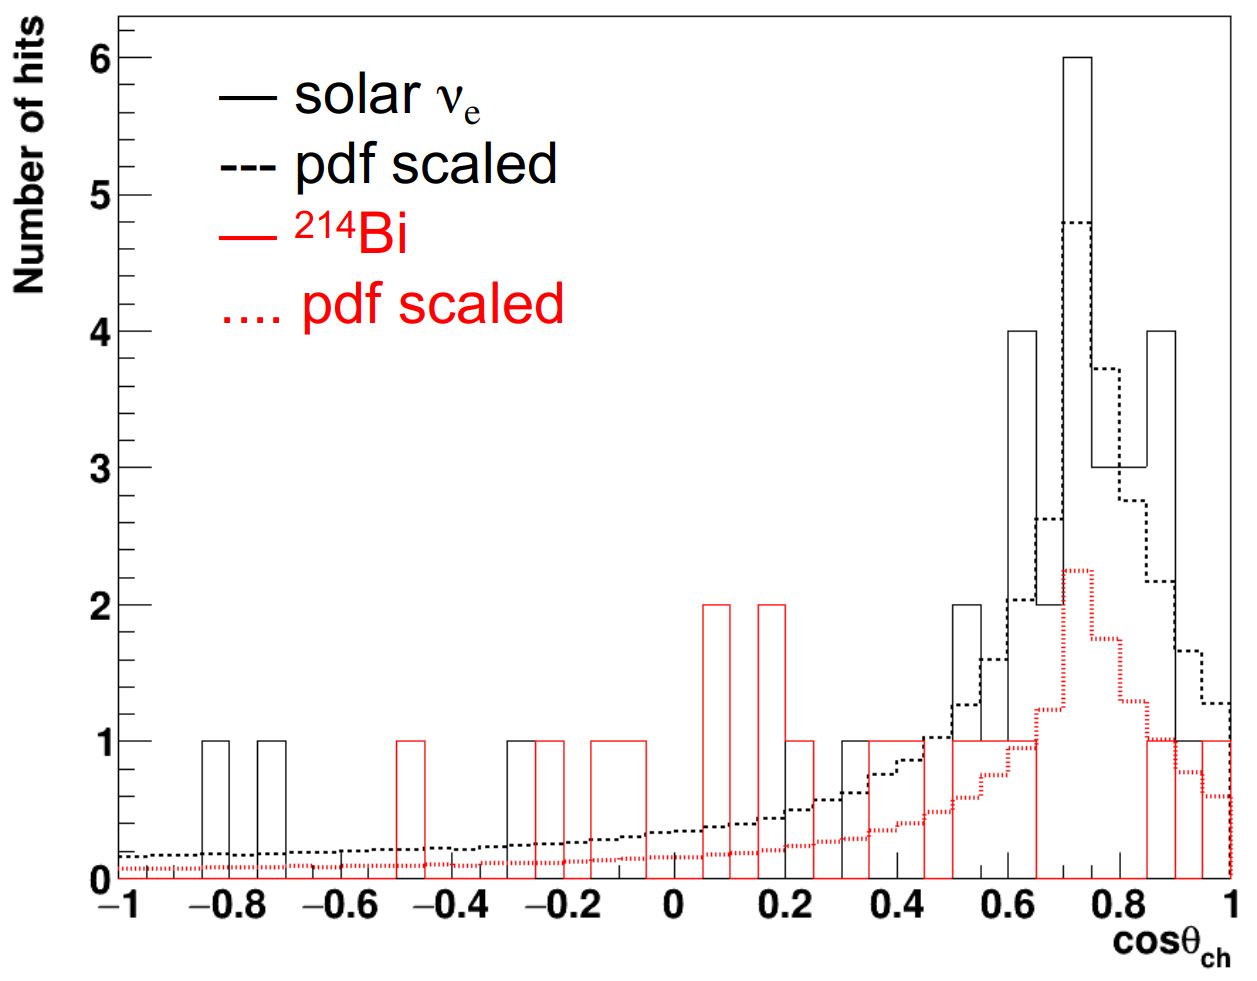
\includegraphics[width=8cm]{klDiv_example.png}
	\caption{Angular distributions of the MC events in run-by-run simulation 206391, with the same event GTID =7. The black line is the MC solar $\nu_e$ distribution, while the red line is the MC $^{214}$Bi distribution. The pdf is scaled to the number of the hits in solar $\nu_e$ event (black dashed line) and the $^{214}$Bi event (red dotted line) respectively.}
	\label{kLdiv_example}
\end{figure}

A symmetrical form of $klDiv$ can be taken as:
\begin{equation}
klDiv(p,q) \equiv \frac{1}{2}\sum_{i}^N (p\log{\frac{p}{q}}+q\log{\frac{q}{p}}),
\end{equation}
Since $klDiv(p,q)=klDiv(q,p)$, it has a meaning of distance. The quantity is not used in the thesis, but can be considered in future.

\section{Solar \texorpdfstring{$\nu_e$}{Lg} Analysis and Background Separation in Water Phase}
\subsection{Open Dataset Analysis}

This open dataset was used to compare the MPW and the RAT fitted results.

In SNO+ water phase, solar $\nu_e$s are basically measured via elastic scattering $\nu_e+e^-\to \nu_e+e^-$. The maximum kinetic energy of the recoil electron is
$T_{max}=\frac{2E^2_\nu}{2E_\nu+m_e c^2}$
the cross section is $\sigma(\nu_e+e^-\to \nu_e+e^-)=9.52\times 10^{-44}(E_\nu/10~MeV)~cm^2$
the expected solar neutrino rate is 
$R=A\int_{T_{thresh}}^{T_{max}}\frac{d\sigma}{dE}\frac{dN}{dE_\nu}dE_\nu$.
A ``solar angle'', $\theta_{sun}$ is the direction of the event relative to the Sun's location,


$\nu-e^-$ elastic scattering: 
\begin{equation}\label{eq:costhetaSun}
\cos\theta_{sun}=\sqrt{\frac{T_e(m_e+E_\nu)^2}{2m_eE_\nu^2+T_eE_\nu^2}}
\end{equation}

For the data, the solar angle is defined as:
\begin{equation}
	\cos\theta_{sun}\equiv \vec u_{event}\cdot \frac{\vec{X}_{event}-\vec{X}_{sun}}{|\vec{X}_{event}-\vec{X}_{sun}|},
\end{equation}
where $\vec{X}_{sun}$ is taken as the Sun's location relative to the SNOLAB location since the whole lab can be treated as a point regarding the long distance to the Sun.



High level cuts mentioned in \ref{sect:high_level_cuts} were applied.

\begin{table}[ht]
	\centering
	\caption{Candidate events in the open dataset. Compared the fitted results of the candidate events with different fitters.}
	\label{opendata}
	\begin{tabular*}{150mm}{c@{\extracolsep{\fill}}cccccccc}
		\toprule
		Fitter &	Run &  GTID &  $z-0.108$(m) & $R$(m)& $(R/R_{av})^3$ & $\cos\theta_{sun}$ & SNO+ Day\\
		\hline 
		Rat & 100093 &11108354 &3.49 &3.57 &0.21 &-0.954 &2683.92 \\	
		MPW &  --& --& 3.43 &	3.52 &	0.20	& -0.906 & --\\
		Rat &	100207 &5079885 &-2.61 &4.60 &0.45 &0.816 &2687.04\\
		MPW &	 --& --& -3.63 & \textbf{7.61} &	2.03 & \textbf{0.656} & -- \\
		Rat &100632 &7882360 &1.77 &3.19 &0.15 &0.937 &2696.93\\
		MPW &    --& --&  1.67 & 3.11 &	0.14 & 0.911 & -- \\
		Rat &100663 &15767175 &-4.33& 4.96 &0.56 &0.978 &2698.18\\
		MPW & --& -- &-4.45 &	5.07 &	0.60 &	0.980 & -- \\
		Rat &100915 &169700 &-1.00 &5.10 &0.61 &0.341 &2701.23\\
		MPW &	--& --& -1.08 &	5.08 &	0.61 &	0.337 & -- \\	
		\bottomrule
	\end{tabular*}
\end{table}

\begin{table}[ht]
	\centering
	\caption{Candidate events in the open dataset, searched by the MPW fitter.}
	\label{opendataMPW}
	\begin{tabular*}{150mm}{c@{\extracolsep{\fill}}cccccccc}
		\toprule
		Run & GTID & energy & $z-0.108$ & $R$ & $(R/R_{av})^3$ & $\cos\theta_{sun}$\\
		\hline 
		100093 &	11108354	&5.827 & 3.43 & 3.52 & 0.20 & -0.907005\\
		100632&	7882360    &6.183& 1.67 &3.11 &0.14 &0.9146124\\
		100663&	15767175   &	6.182 & -4.45 &5.07 &0.60&	0.9807349\\
		100915&	169700   &	5.684 &	-1.07 &5.08 &0.61&0.3385341\\
		100984&	8621621&	5.701 & 0.76 &4.75 &0.502&-0.647735\\
		101075&	11673714&	5.667 &4.43 &5.18 &0.64& 0.5873025\\
		
		\bottomrule
	\end{tabular*}
\end{table}
solar neutrino candidate events in the open dataset.

\begin{figure}[htbp]
	\centering
	\subfigure[Run 100093, GTID 11108354]{ 
		\begin{minipage}[t]{0.4\textwidth}
			\centering
			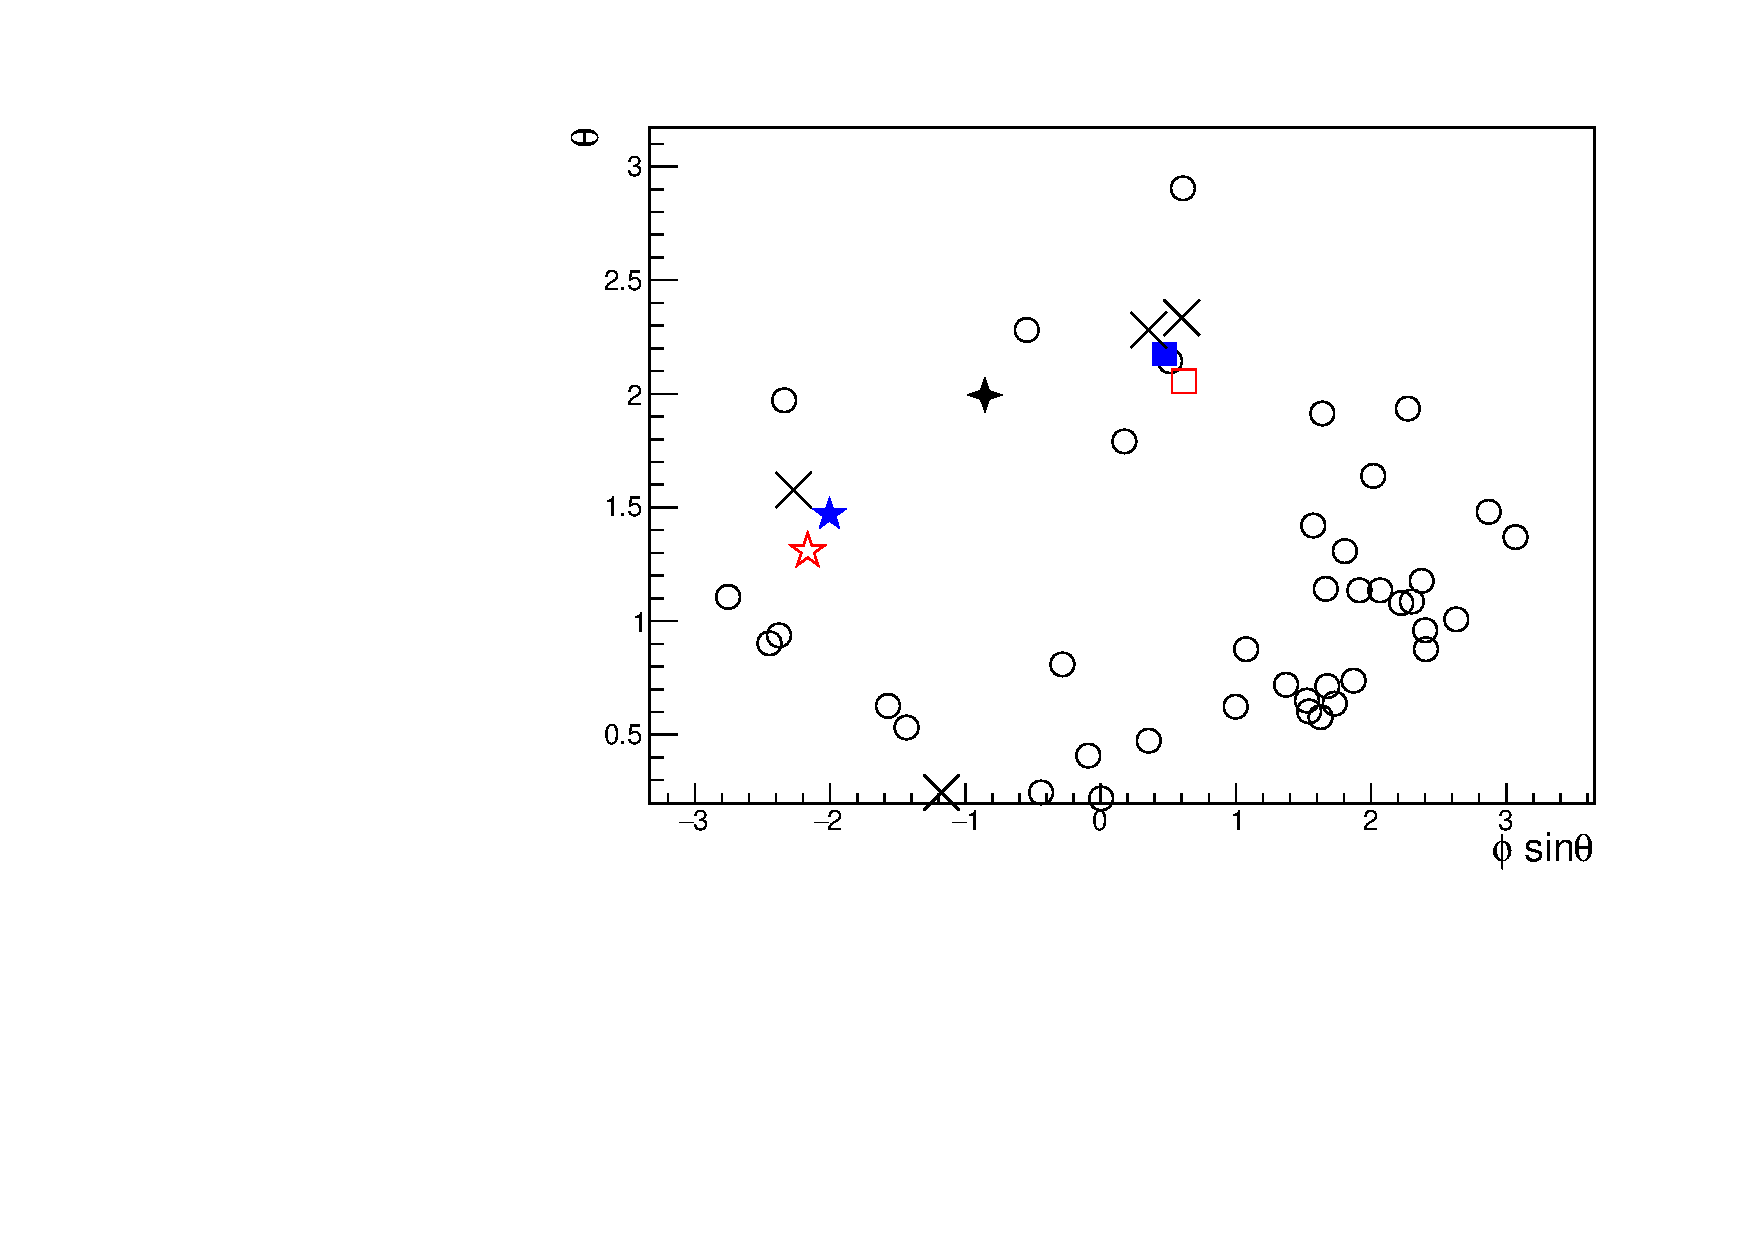
\includegraphics[width=6cm]{PMTmap_100093.pdf}
		\end{minipage}
	}
	\subfigure[Run 100207, GTID 5079885]{ 
		\begin{minipage}[b]{0.4\textwidth}
			\centering
			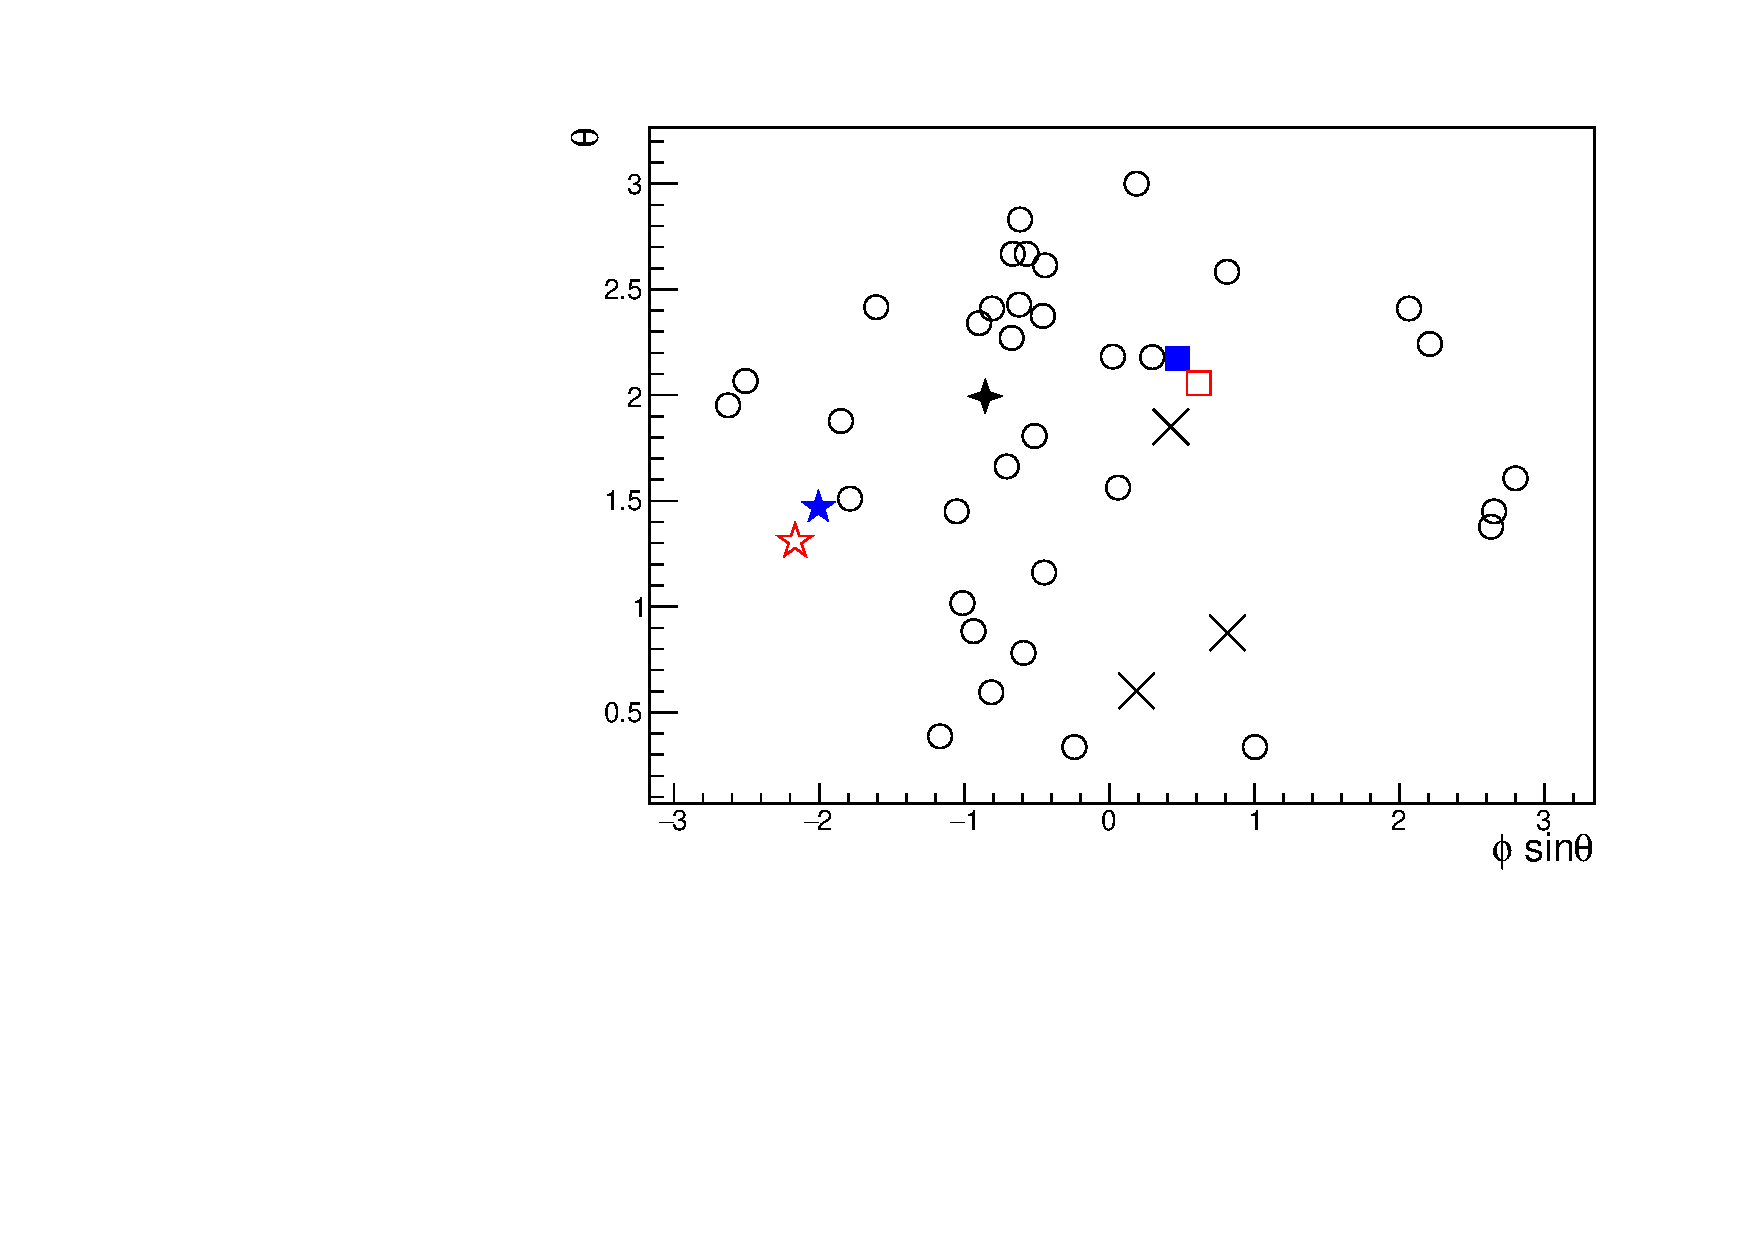
\includegraphics[width=6cm]{PMTmap_100207.pdf}
		\end{minipage}
	}
	\subfigure[Run 100632, GTID 7882360]{ 
		\begin{minipage}[t]{0.4\textwidth}
			\centering
			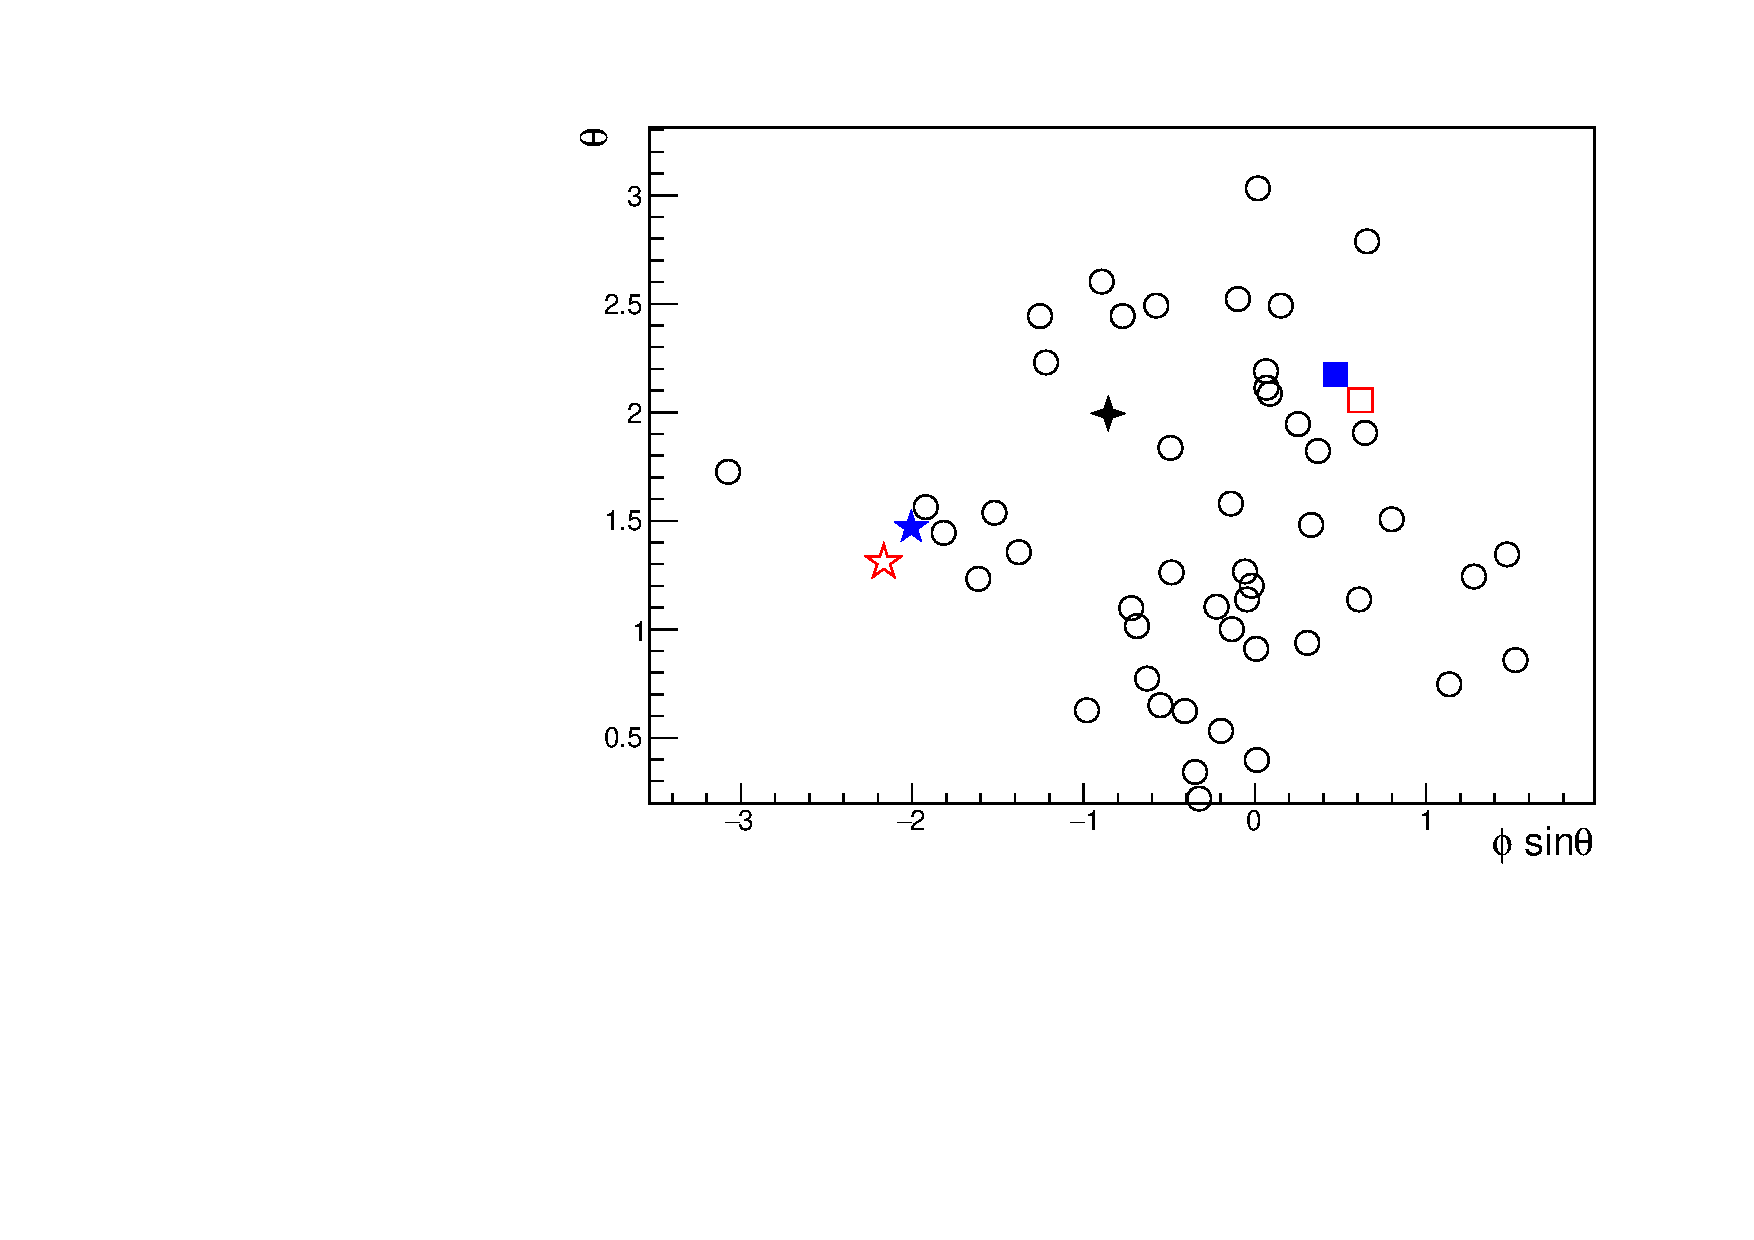
\includegraphics[width=6cm]{PMTmap_100632.pdf}
		\end{minipage}
	}
	\subfigure[Run 100663, GTID 15767175]{ 
		\begin{minipage}[t]{0.4\textwidth}
			\centering
			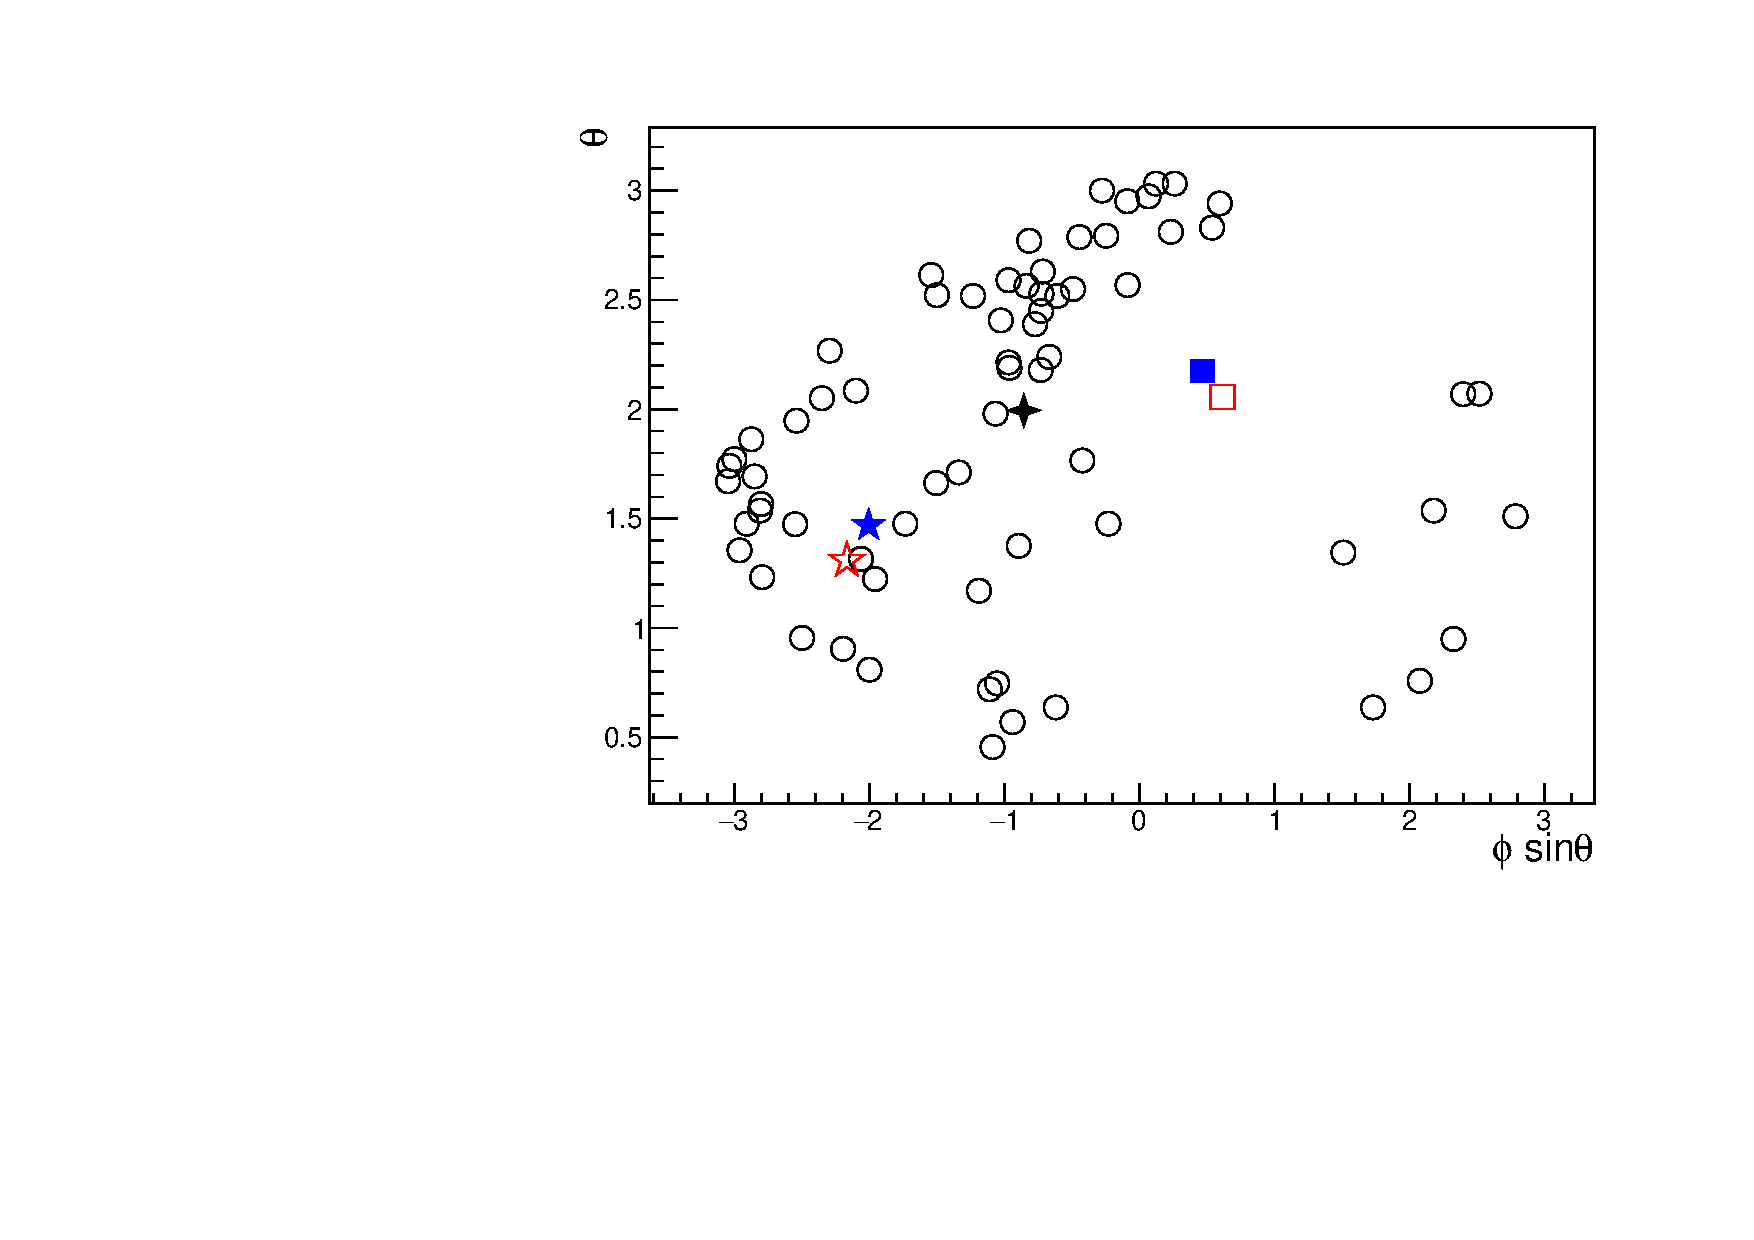
\includegraphics[width=6cm]{PMTmap_100663.pdf}
		\end{minipage}
	}
	\subfigure[Run 100915, GTID 169700]{ 
		\begin{minipage}[t]{0.4\textwidth}
			\centering
			{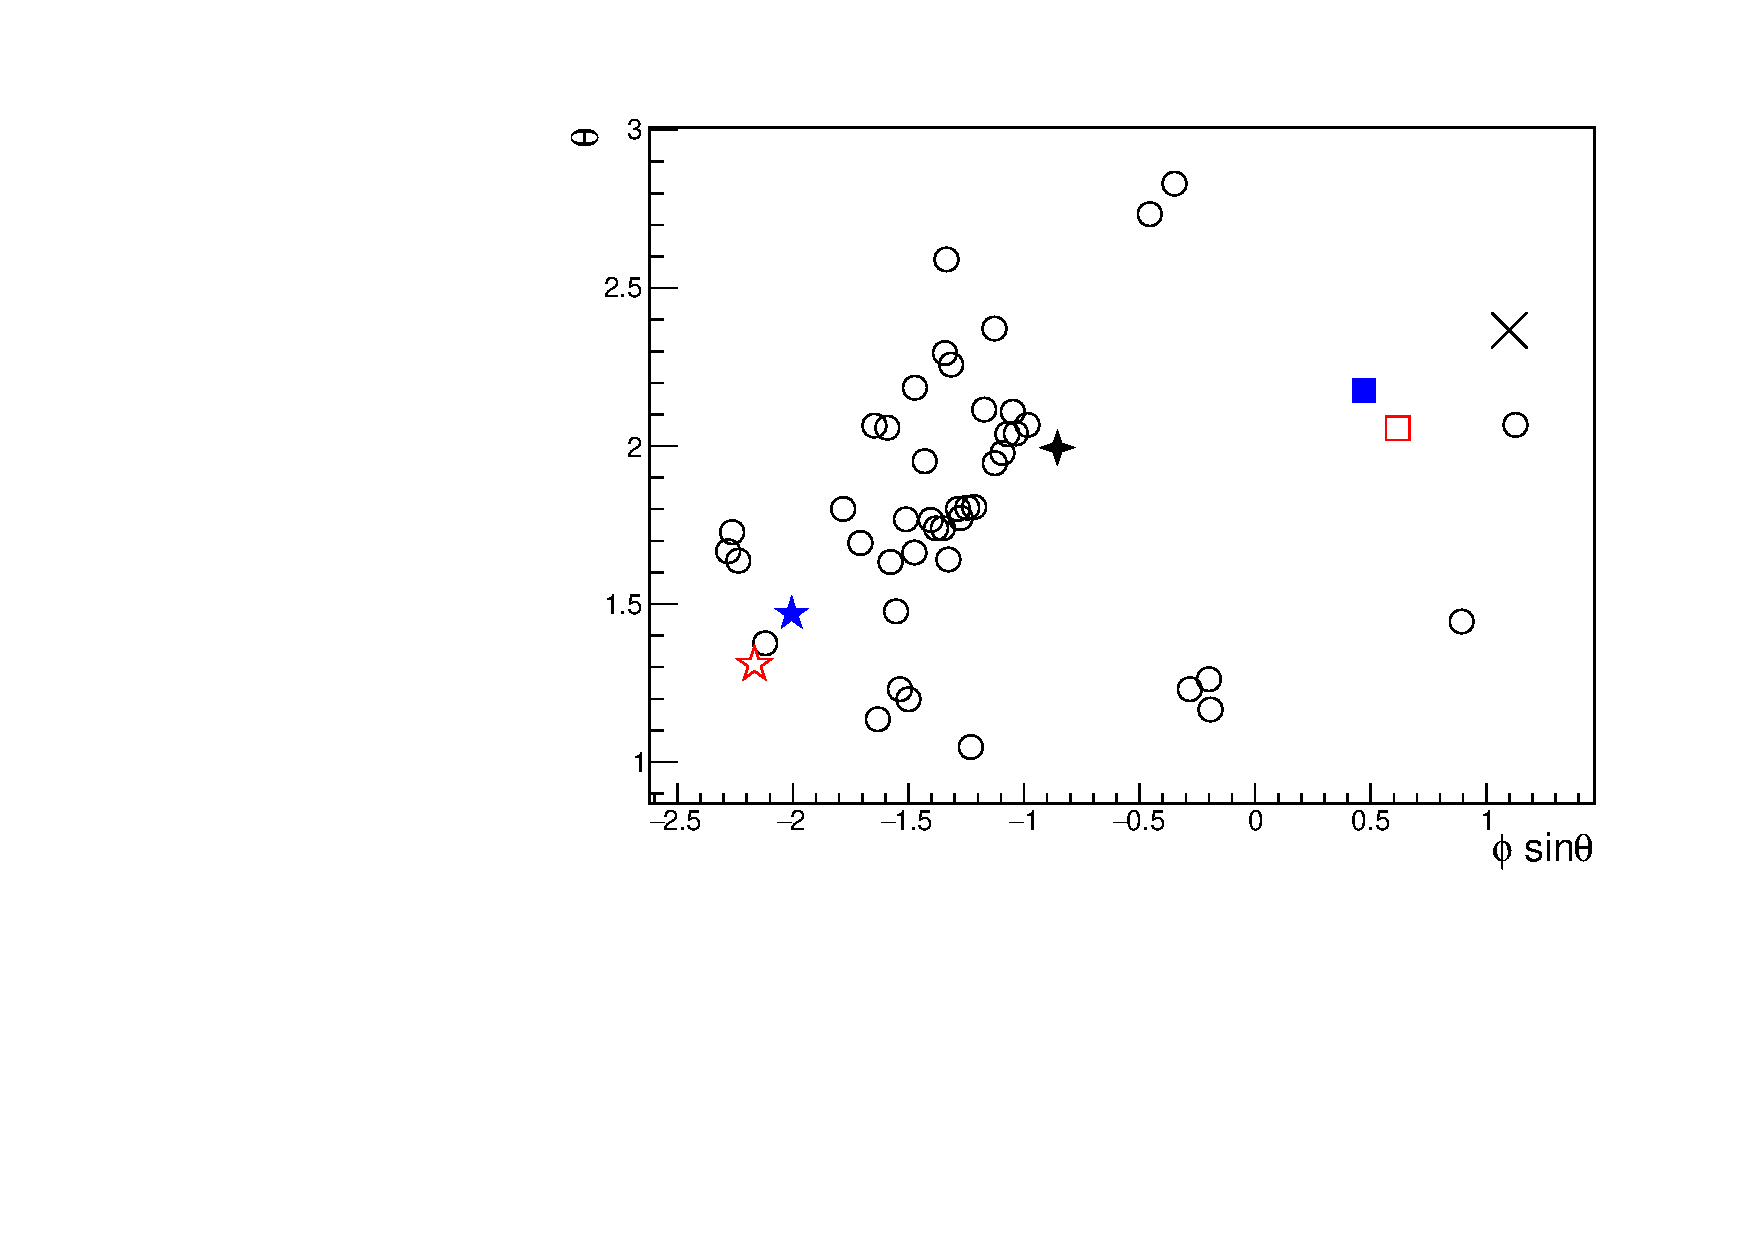
\includegraphics[width=6cm]{PMTmap_100915.pdf}}
		\end{minipage}
	}
	\subfigure[Legends]{ 
		\begin{minipage}[b]{0.4\textwidth}
			\centering
			{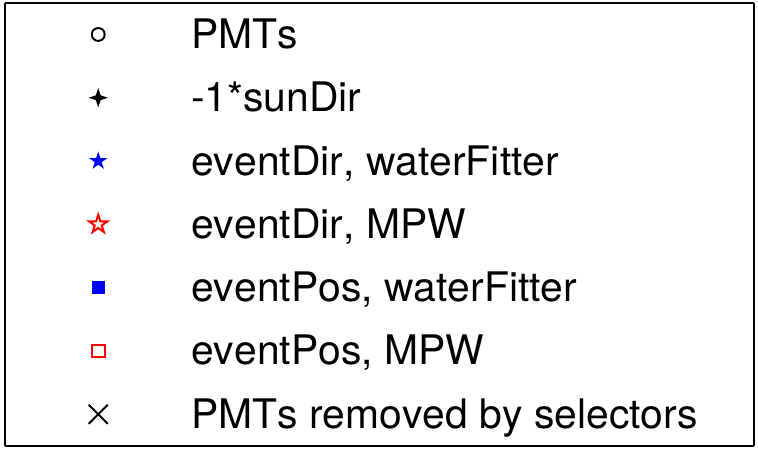
\includegraphics[width=5cm]{solarLegends.png}}
		\end{minipage}
	}
	\caption{Fit results for the candidate events, projected onto PMT sinusoidal maps. Black circles stand for
		the hit PMTs used by the fitter; crosses stand for the hit PMTs removed by the selectors; blue full star stands for the event direction fitted by the waterFitter; red open star stands for the direction fitted by the MPW; full double diamond stands for the solar direction*-1; blue full square stands for the event position fitted by the waterFitter; open square stands for the position fitted by the MPW.}
	\label{openDataSetCandidate}
\end{figure}

Compare the $klDiv$ quantities for the MPW and RAT results. 

A plot of refitting the RAT candidate solar events with the MPW on old dataset.



\subsection{TMVA Analysis}\ref{sect:tmva}
The MC simulations of the runs 200004 to 203602 were used. These run-by-run simulations simulated the full detector conditions for every run. This is a sub-dataset to the whole ``low background dataset'', with a live time of 92.54 days for testing and training the TMVA methods.

Two types of background isotopes, $^{208}$Tl and $^{214}$Bi were simulated in different detector regions. In this study, the background events simulated in the inner AV (internal backgrounds) , in the AV and in the external water region were checked. The solar $\nu_e$ events simulated in the inner AV were used as signals. Table.~\ref{table:mixed_MC} summarizes the types of simulations used in this study. 
\begin{table}[ht]
	\centering
	\caption{Datasets of MC simulations.}
	\label{table:mixed_MC}
	\begin{tabular*}{100mm}{c@{\extracolsep{\fill}}cccccccc}
		\toprule
		Simulations & Simulated positions in the detector\\
		\hline 
		$^{208}$Tl & inner AV (internal $^{208}$Tl)\\
		-- & AV \\
		-- & external water (external $^{208}$Tl)\\
		\midrule
		$^{214}$Bi & inner AV (internal $^{214}$Bi)\\
		-- & AV \\
		-- & external water (external $^{214}$Bi)\\
		\midrule
		Solar $\nu_e$ & inner AV (internal $\nu_e$)\\
		-- & AV \\
		-- & external water (external $\nu_e$)\\
		\bottomrule
	\end{tabular*}
\end{table}

Different types of the simulations were merged into a mixed dataset. The simulated solar $\nu_e$ events are tagged as signals and mixed with $^{214}$Bi and $^{208}$Tl background events. The total dataset was divided into training and testing sets. 

Fig.~\ref{TMVA_bkgs_1} shows the energy spectrum of simulated internal events with their fitted positions inside the 5.5-m fiducial volume, i.e., with a radial cut of $R'_{fit}<5.5~m$, where the $R'_{fit}$ is the magnitude of the reconstructed event position $\vec{X}_{fit}$ after the AV coordinate correction: $R'_{fit}\equiv\sqrt{x^2_{fit}+y^2_{fit}+(z_{fit}-108)^2}$. The 108 mm offset in $z$ was discussed in Chapter 3 and Chapter 4. 

\begin{figure}[!htb]
	\centering
	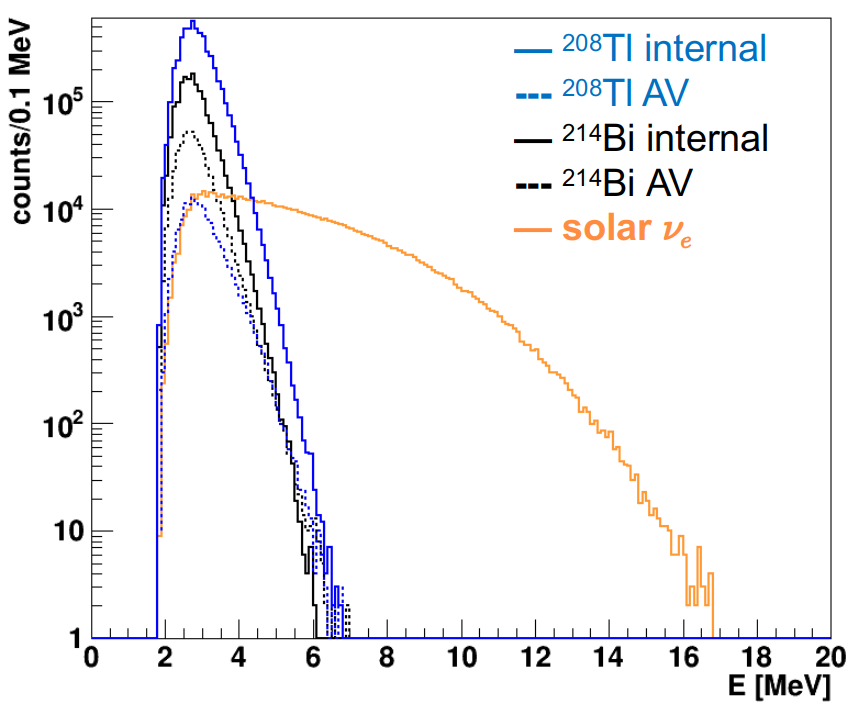
\includegraphics[width=8cm]{TMVA_bkgs_1.png}
	\caption{Energy spectrum of the simulated events for $^{214}$Bi (black), $^{208}$Tl (blue) and solar $\nu_e$ (orange). Solid lines show the internal events and dotted lines show the AV events.}
	\label{TMVA_bkgs_1}
\end{figure}

In this sub-dataset, runs from 201700 to 202516 were taken as the training set (69.5\% of the total sub-dataset), and the rest 30.5\% were taken as testing set. Once the weights of the variables were tuned, they were put into the actual data.

Before the analysis, a few ``beforehand cuts''were applied: $NHits>20$, $R'_{fit}<5500~mm$, $ITR>0.55$, $-0.12<\beta_{14}<0.95$. Here $NHits>20$ was applied as a reconstruction threshold. Only the events with $NHits>20$ were reconstructed by the MPW fitter for the solar neutrino analysis; a default fiducial volume of $5.5~m$ was set; the $ITR$ and $\beta_{14}$ cuts were suggested by the collaboration, which were mostly based on the experiences for removing the instrumental backgrounds\cite{waterunidoc}. 

Distributions of input variables:
signal vs combined backgrounds


After applying these beforehand cuts, for $4<E_{fit}<15~MeV$, the training dataset had 416780 events and the testing dataset had 184330 events.

Two other ranges of $E_{fit}$ were also tested: $4<E_{fit}<5$ (low energy region) and $5<E_{fit}<15$ ($E>5$ region). %$6<E_{fit}<15$ ($E>6$).

After the training and testing datasets were ready, three classification methods implemented in the TMVA package were used: the Fisher discriminants/linear discriminant analysis (Fisher/LD), the Boosted Decision Tree (BDT), and the Artificial Neural Networks Multilayer Perceptron (ANN-MLP, or MLP in short)\cite{albertsson2007tmva}.

The Fisher discriminant $y_{F_i}(i)$ for classifying event $i$ is defined by \cite{tmvaWebsite}:
\begin{equation}
y_{F_i}(i) = F_0+\sum_{k=1}^{n_{params}}F_k x_k(i),
\end{equation}
where $n_{params}$ is the number of input variables; the Fisher coefficients, $F_k$ is given by:
\begin{equation}
F_k = \frac{\sqrt{N_SN_B}}{N_S+N_B}\sum_{l=1}^{n_{params}}1/W_{kl}(\bar{x}_{S,l}-\bar{x}_{B,l}),
\end{equation} 
where $N_{S(B)}$ are the number of signal (background) events in the training sample; $\bar{x_{S(B),l}}$ are the means of input variables for signal (background); $W_{kl}$ is the covariance matrix\cite{tmvaWebsite}.

For the BDT method, the adaptive boosting (AdaBoost) algorithm was used; 400 trees were trained with a maximum depth of 3; gini index was used for the decision tree.

For the MLP method, sigmoid function was set as the activate function; 4 hidden layers, 200 training cycles were used.

I used 9 variables as inputs: $ITR$, $\beta_{14}$, $E_{fit}$, $G_{test}$, $U_{test}$, $scaleLogL$, $Z_{factor}$, $\vec{u}\cdot \vec{R}$ and $klDiv$. Among them, the input values of $ITR$ and $\beta_{14}$ were after the beforehand cuts mentioned above. The $NHits$ and $\theta_{ij}$ were not used, since the $NHits$ is correlated to the energy while the $\theta_{ij}$ is anticorrelated to the $\beta_{14}$.

The MLP method gave the best results, while it was the most CPU-consuming method.

The output signal/background distributions on the test sub dataset are shown in Fig.~\ref{output_separation_allE}.
\begin{figure}[htbp]
	\centering
	\subfigure[Fisher/LD output.]{
		\begin{minipage}[t]{0.4\textwidth}
			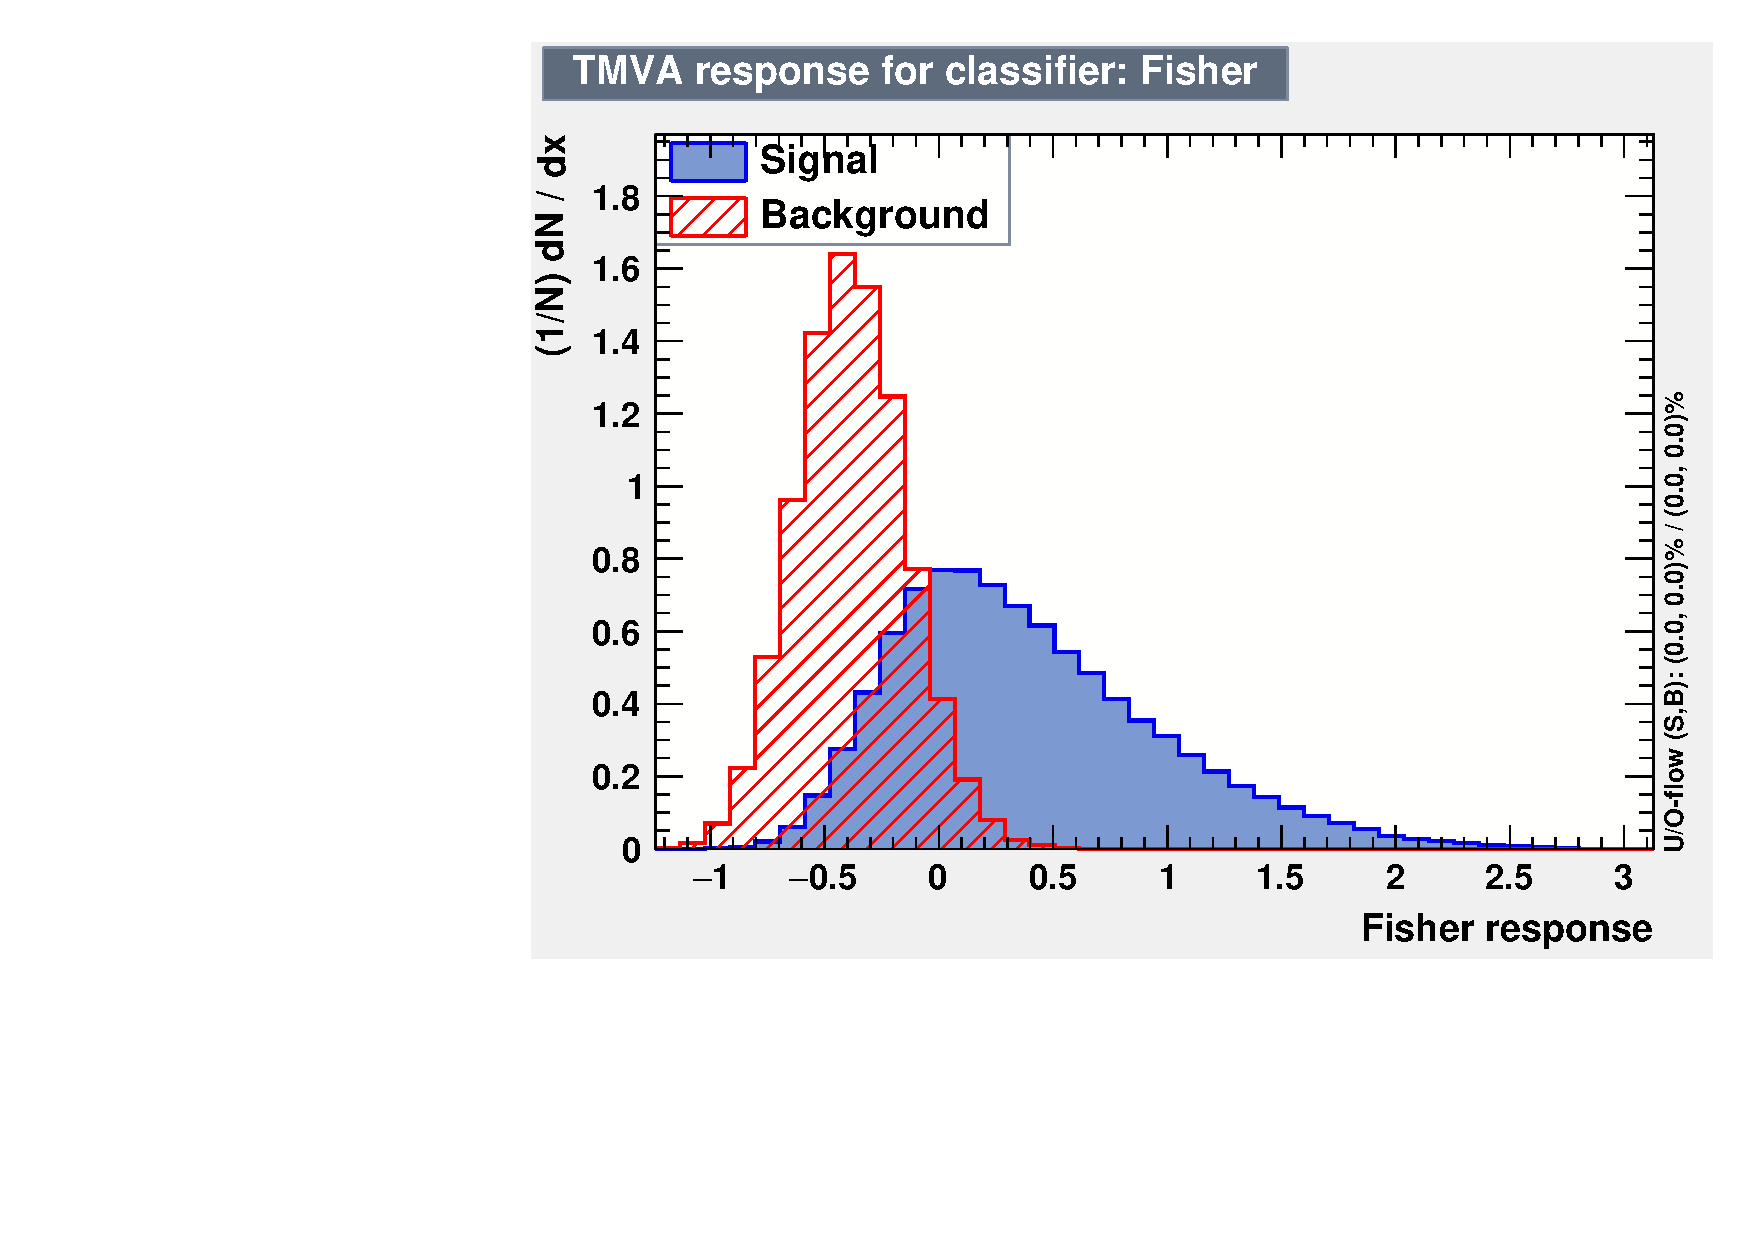
\includegraphics[width=6cm]{output_allE_Fisher.pdf}
		\end{minipage}
	}
	\subfigure[BDT output.]{
		\begin{minipage}[b]{0.4\textwidth}
			\centering
			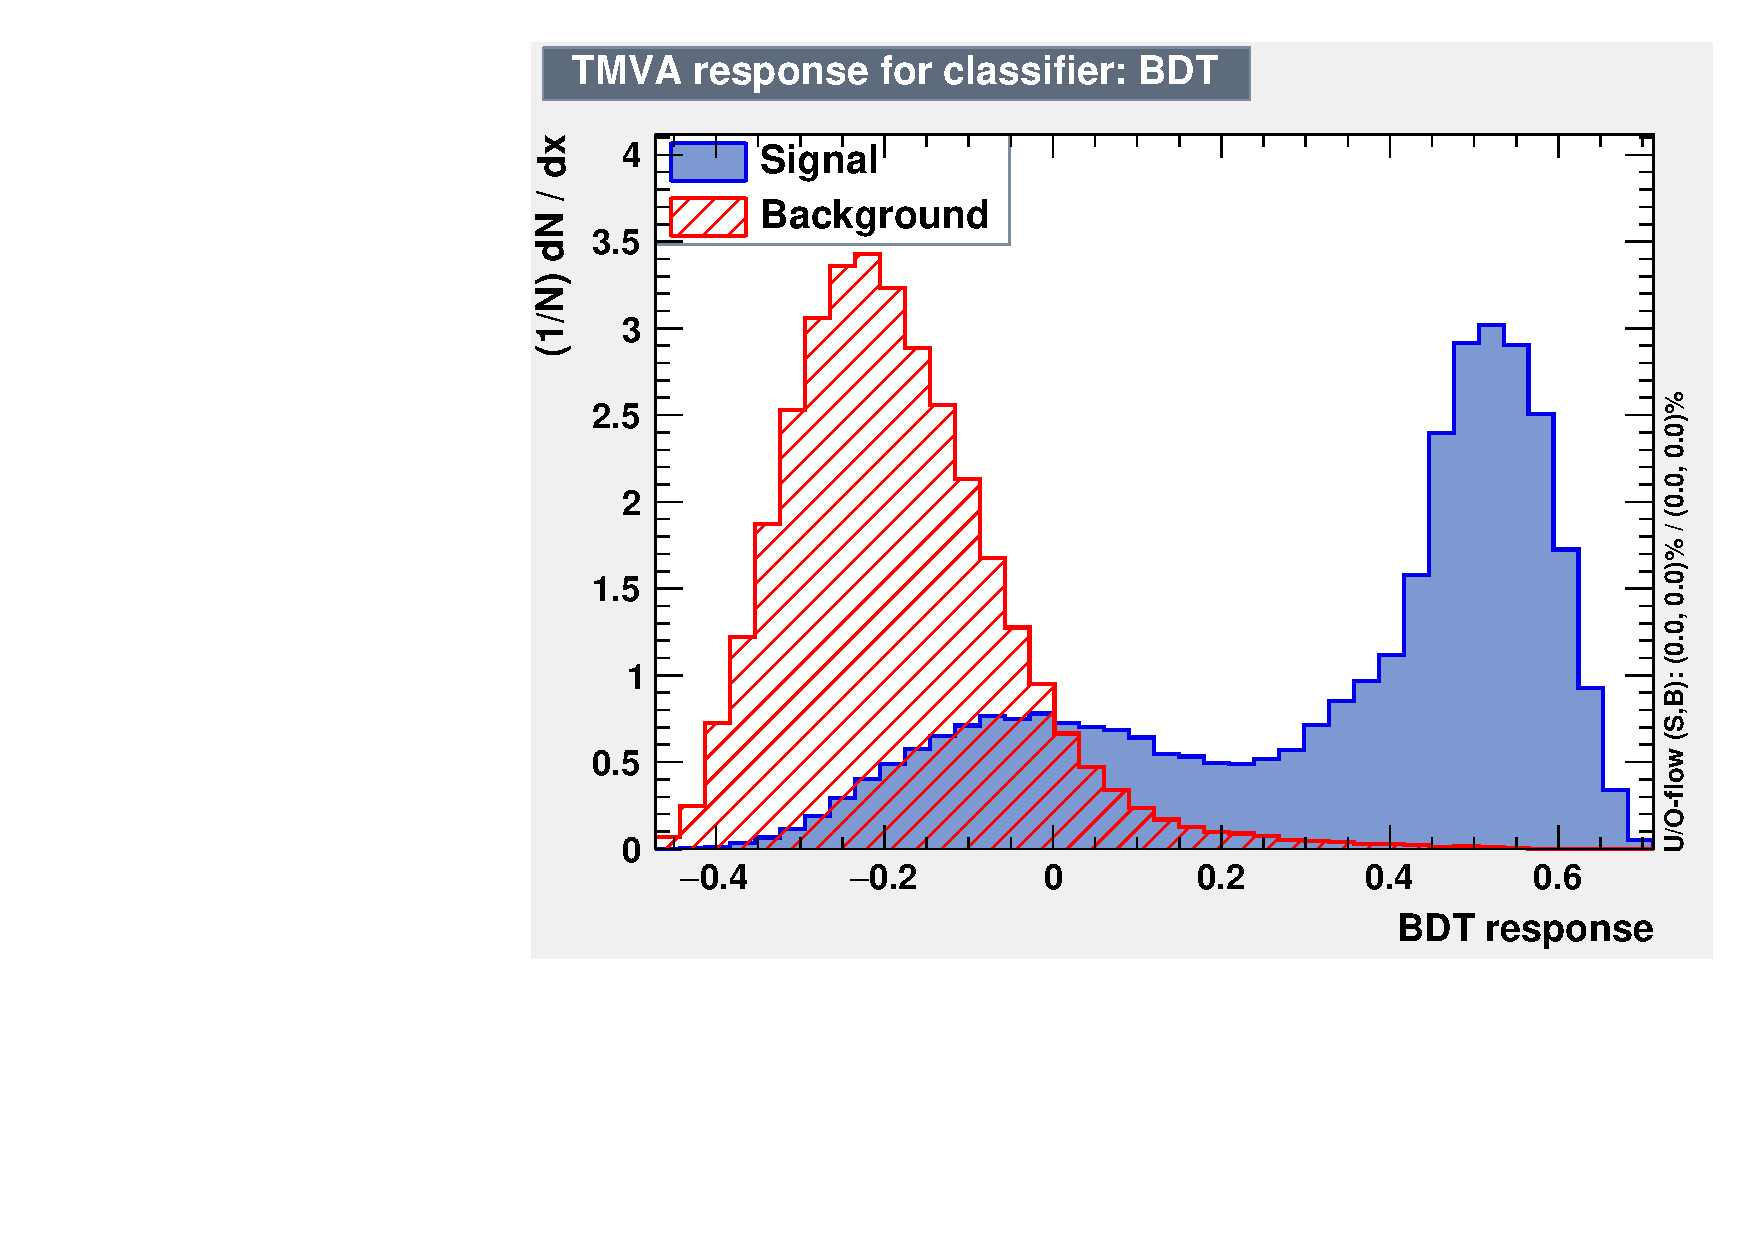
\includegraphics[width=6cm]{output_allE_BDT.pdf}
		\end{minipage}
	}
	\subfigure[MLP output]{
		\begin{minipage}[b]{0.4\textwidth}
			\centering
			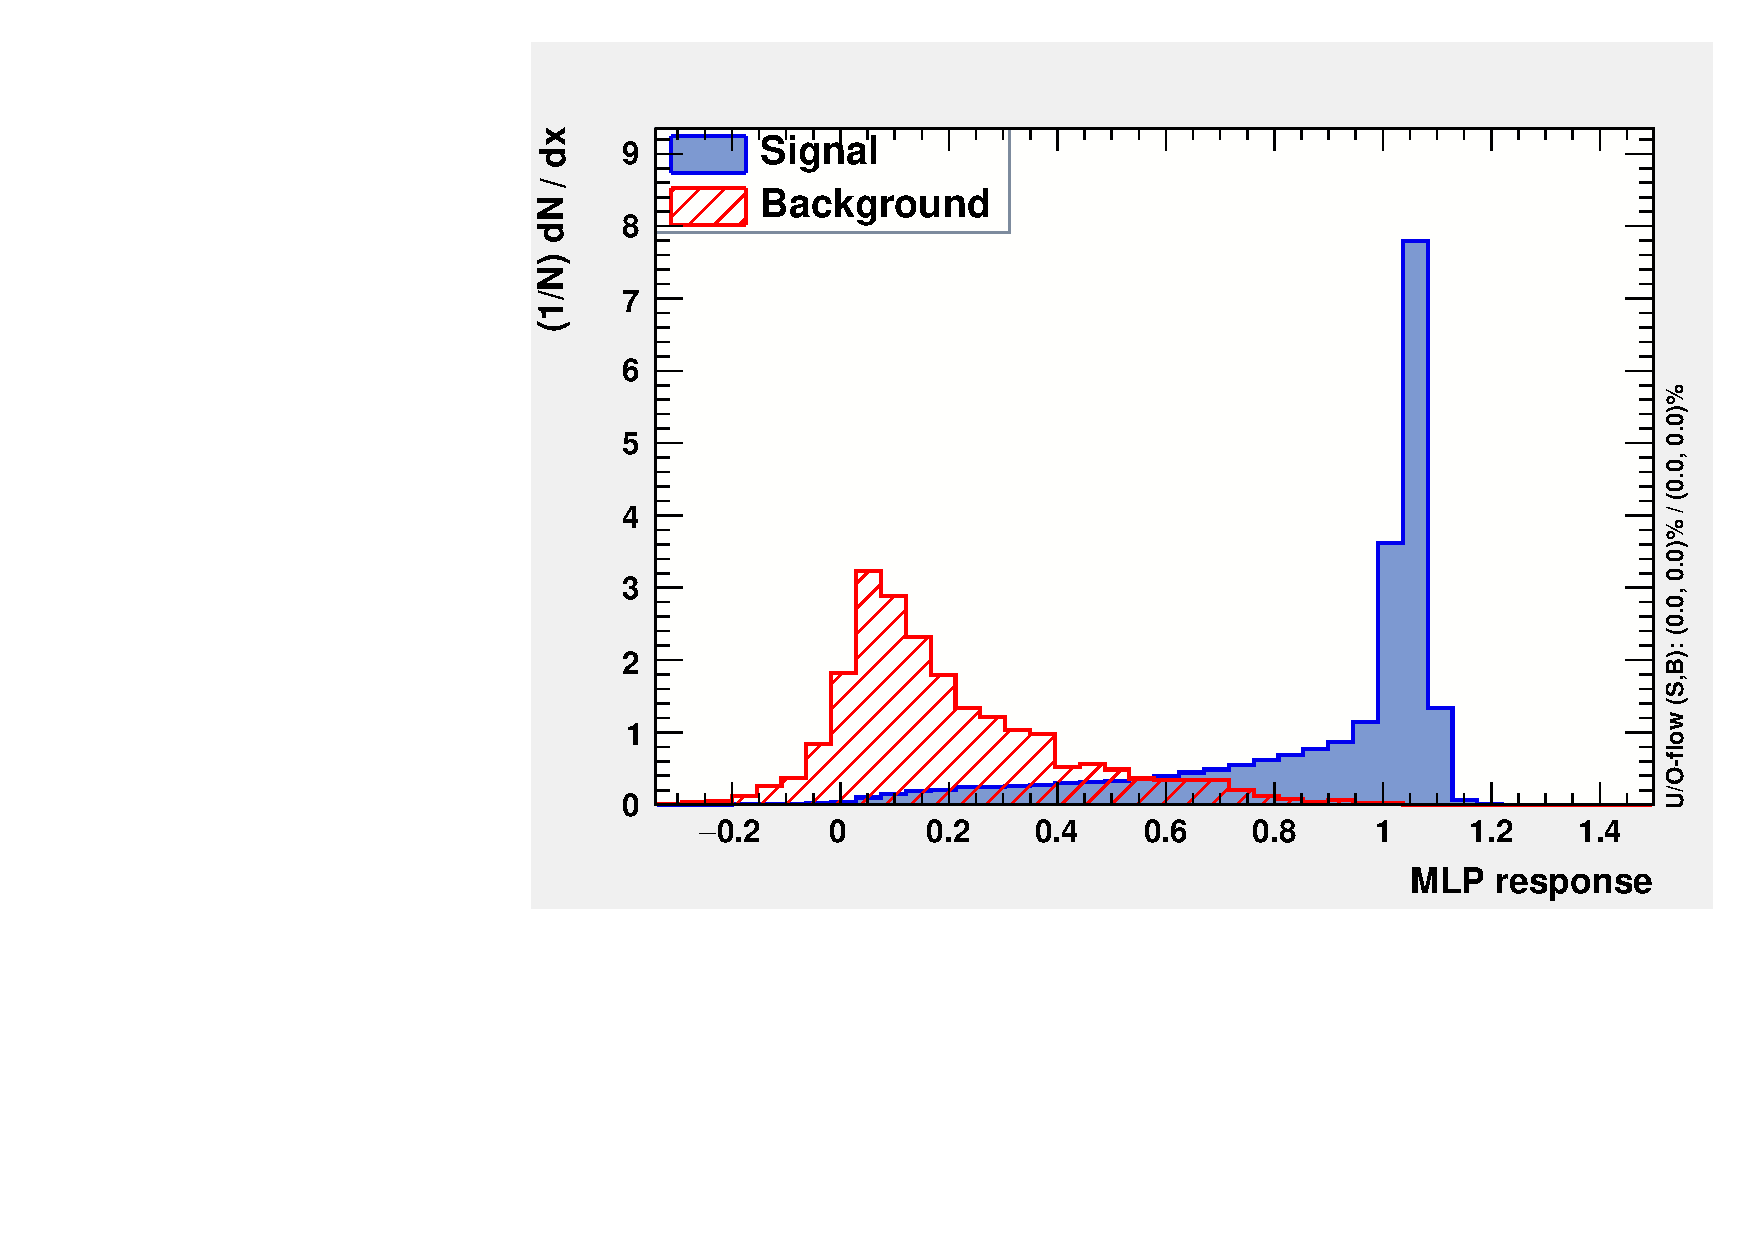
\includegraphics[width=6cm]{output_allE_MLP.pdf}
		\end{minipage}
	}
	\caption{TMVA outputs for signal/background separations by different methods.}
	\label{output_separation_allE}
\end{figure}

As one of the essential TMVA output, the background rejection versus signal efficiency curve is also called a receiver operating characteristic (ROC) curve, which is usually used to test the performance of machine learning classifier. A quantity taking the integrals of the ROC curve: called the ``area under the curve'' (AUC) is often used to summarize the quality of a ROC curve\cite{murphy2012machine}.  Fig.~\ref{allE_roc} shows the ROC curves for different methods:
\begin{figure}[!htb]
	\centering
	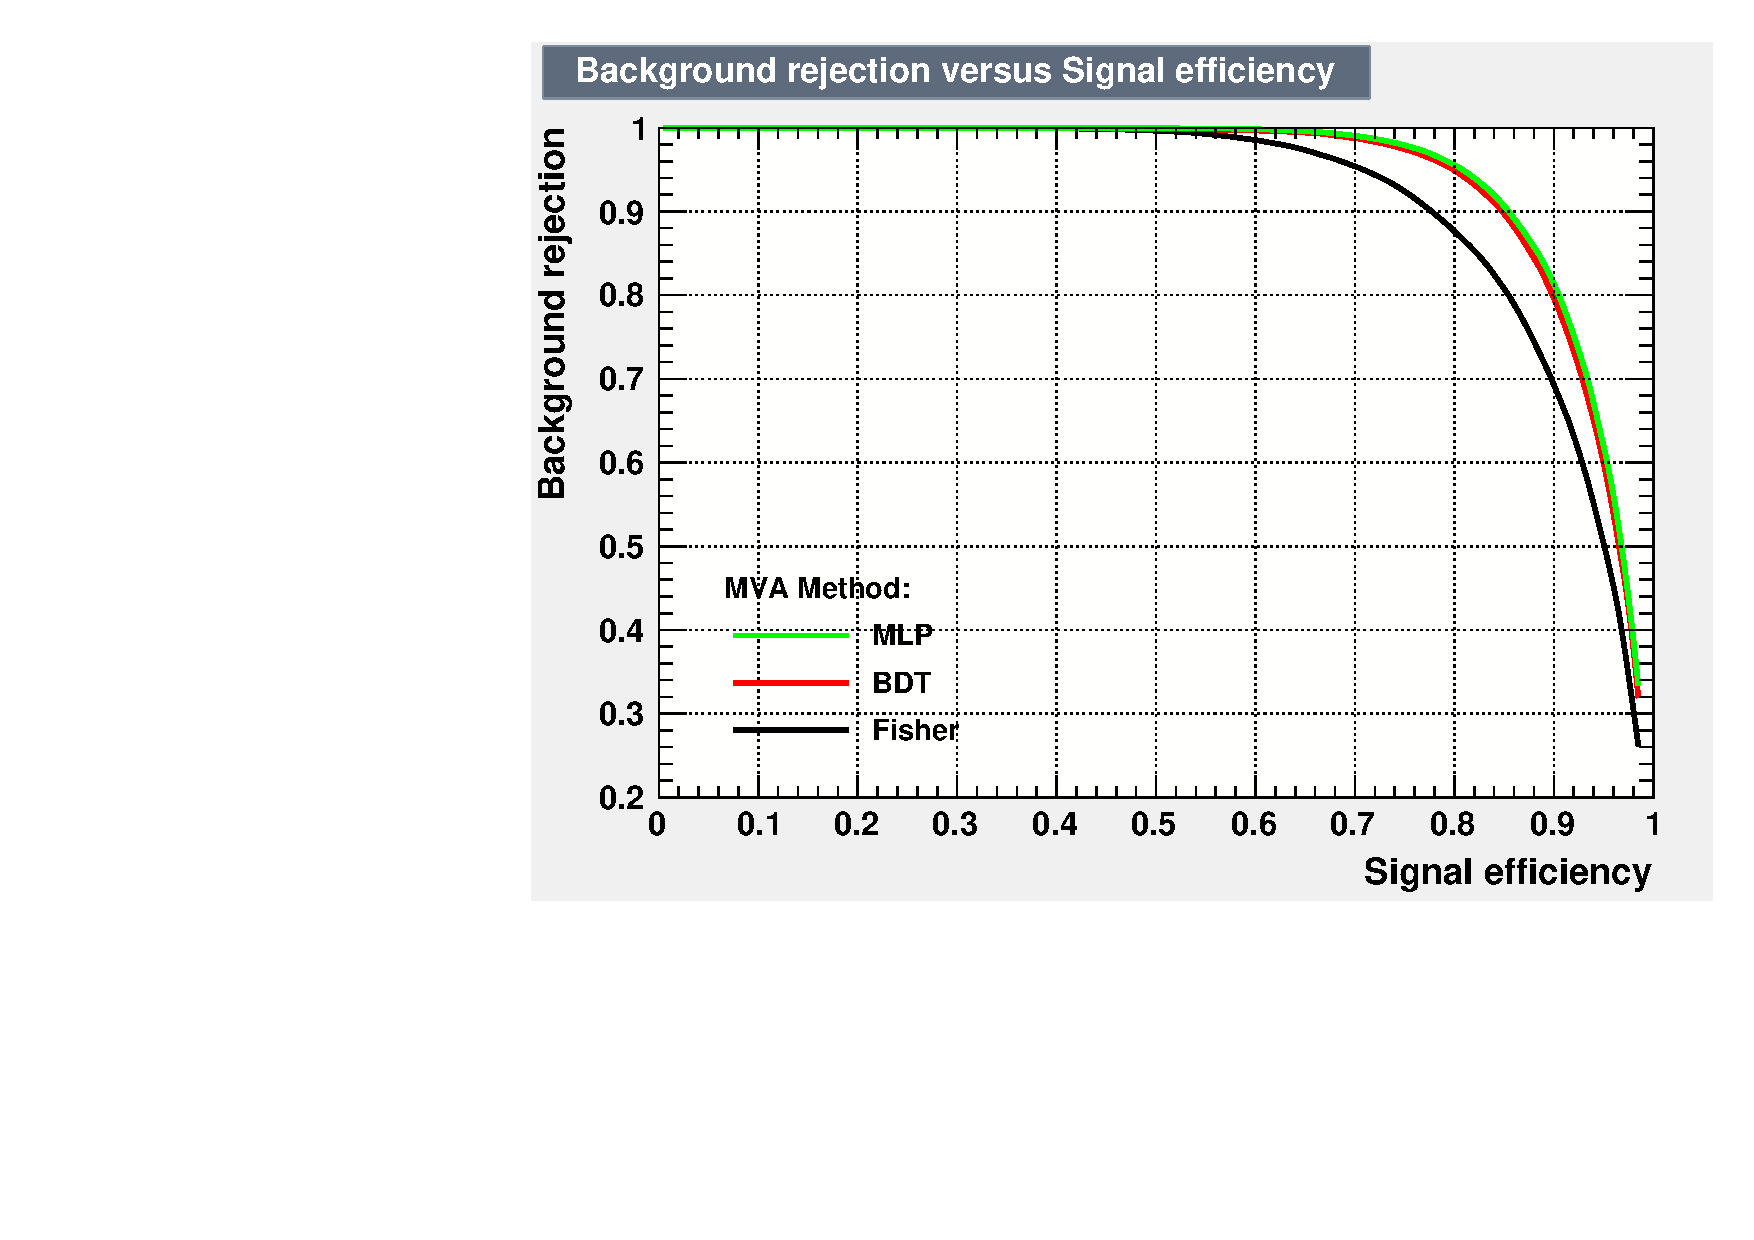
\includegraphics[width=10cm]{ROC_E4to15.pdf}
	\caption{ROC curves from TMVA output, for event with $4<E_{fit}<15~MeV$.}
	\label{allE_roc}
\end{figure}
where the Fisher/LD is the worst case; the BDT and MLP outputs are close to each other while the MLP gives the largest AUC values.

\begin{figure}[!htb]
	\centering
	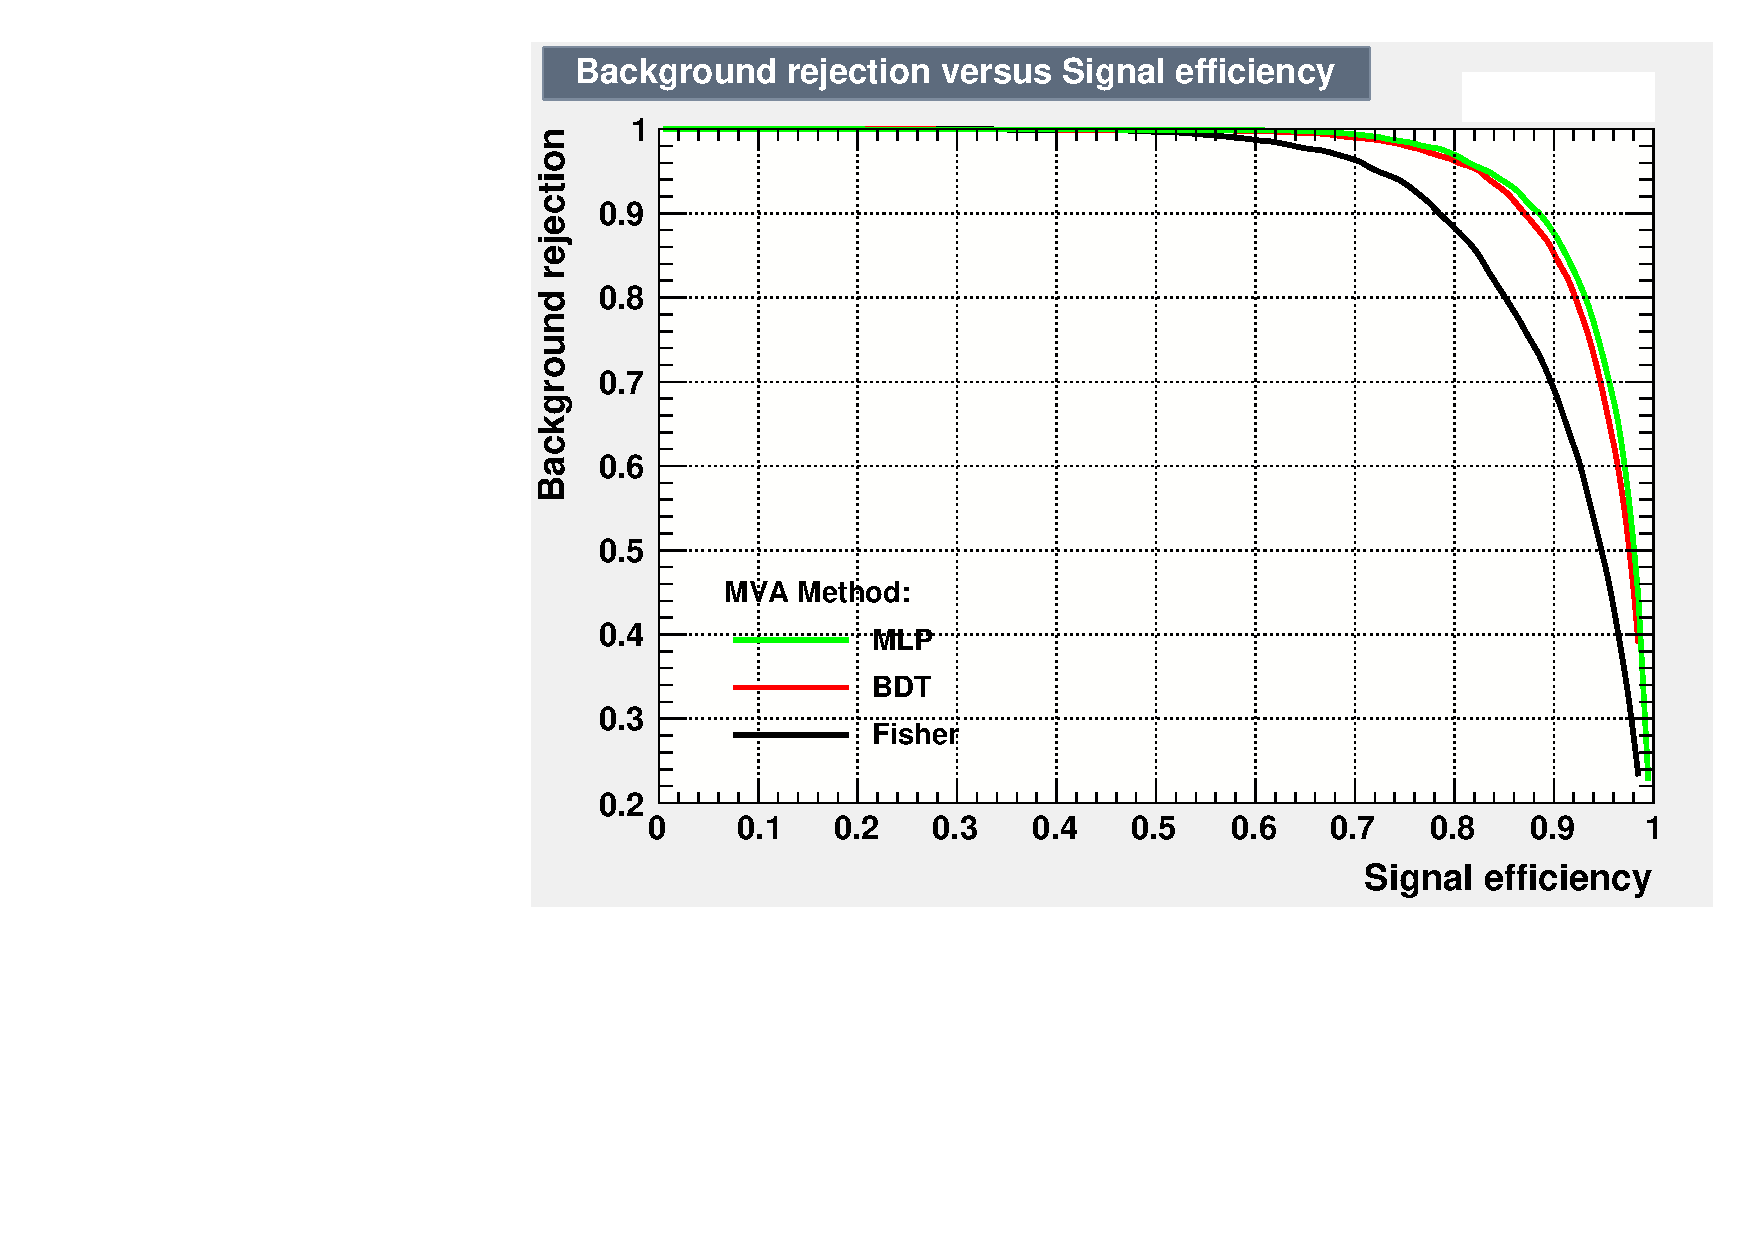
\includegraphics[width=10cm]{ROC_E5to15.pdf}
	\caption{ROC curves from TMVA output, for event with $5<E_{fit}<15~MeV$ (energy above 5 MeV).}
	\label{E5to15_roc}
\end{figure}

\begin{figure}[!htb]
	\centering
	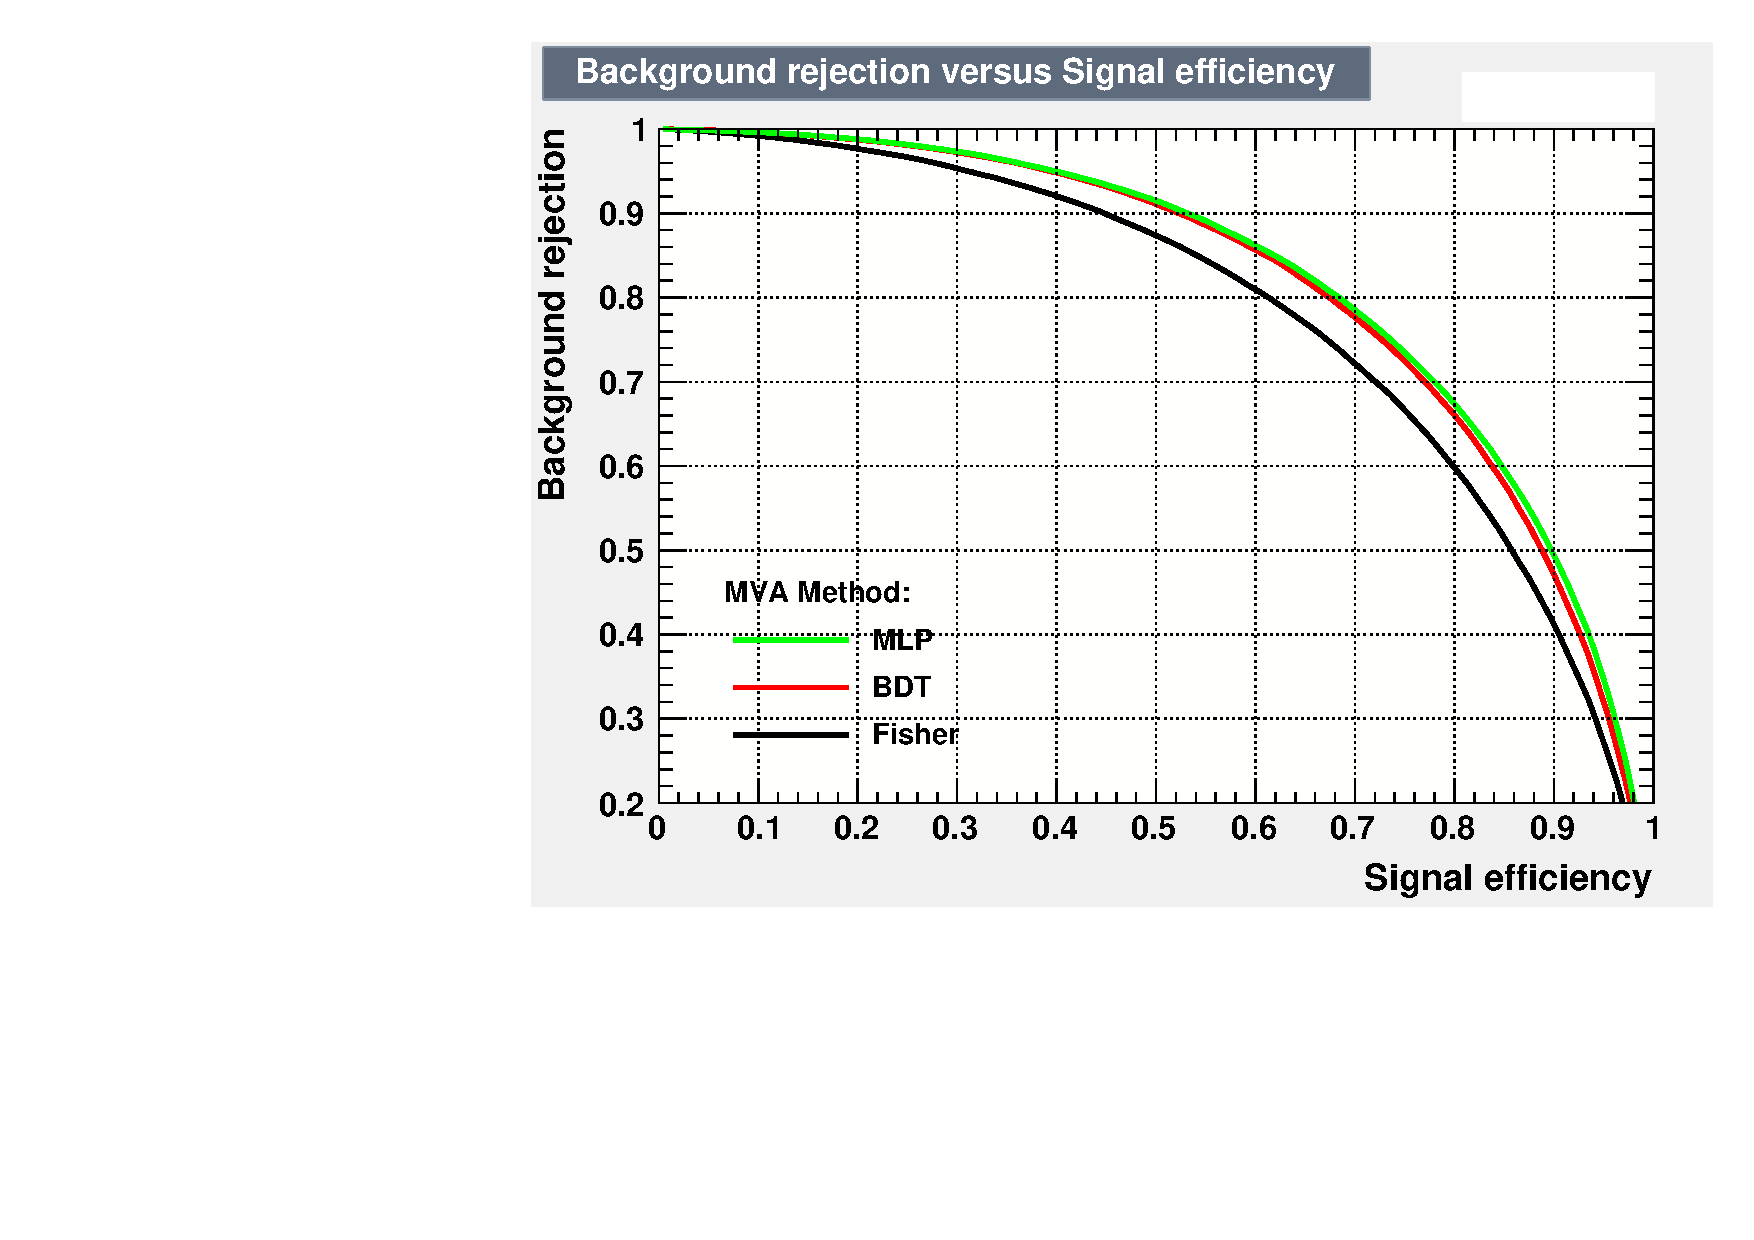
\includegraphics[width=10cm]{ROC_E4to5.pdf}
	\caption{ROC curves from TMVA output, for event with $4<E_{fit}<5~MeV$ (low energy region).}
	\label{E4to5_roc}
\end{figure}

A typical CPU time for a certain method to train the dataset is listed in Table.~\ref{table:tmvaMethod_allE}, \ref{table:tmvaMethod_hiE} and \ref{table:tmvaMethod_lowE}.

\begin{table}[ht]
	\centering
	\caption{Testing results of $4<E_{fit}<15~MeV$ from different TMVA methods.}
	\label{table:tmvaMethod_allE}
	\begin{tabular*}{100mm}{c@{\extracolsep{\fill}}ccc}
		\toprule
		Method & AUC &CPU time (second/$10^6$ events) \\
		\midrule
		Fisher/LD & 0.915 & 0.81\\
		BDT &  0.940 & 249.53 \\
		MLP & 0.944 & 1370.02\\
		\bottomrule
	\end{tabular*}
\end{table}

\begin{table}[ht]
	\centering
	\caption{Testing results of $5<E_{fit}<15~MeV$ (above 5 MeV) from different TMVA methods.}
	\label{table:tmvaMethod_hiE}
	\begin{tabular*}{100mm}{c@{\extracolsep{\fill}}ccc}
		\toprule
		Method & AUC &CPU time (second/$10^6$ events)\\
		\midrule
		Fisher/LD & 0.915& 0.93\\
		BDT & 0.950 & 269.71\\
		MLP &  0.958 & 1450.90\\
		\bottomrule
	\end{tabular*}
\end{table}

\begin{table}[ht]
	\centering
	\caption{Testing results of $4<E_{fit}<5~MeV$ (low energy region) from different TMVA methods.}
	\label{table:tmvaMethod_lowE}
	\begin{tabular*}{100mm}{c@{\extracolsep{\fill}}cccc}
		\toprule
		Method & AUC & CPU time (second/$10^6$ events) \\
		\midrule
		Fisher/LD & 0.782 & 0.84\\
		BDT & 0.816 & 280.1\\
		MLP & 0.823 &1337.9\\
		\bottomrule
	\end{tabular*}
\end{table}

It shows that, when the energy goes lower, it is more difficult to separate the signals from the backgrounds.

The distributions of the ``solar angle'', $\cos\theta_{sun}$ were used to show the performance of the solar $\nu_e$ event selection and background event discrimination. It is also used to extract the number of signal and background events, which will be discussed in the following sections. Here I applied the BDT and the MPL method on the test sub dataset. For the real dataset from run-200004 to 207718, the trained weights and variables from the BDT and the MLP methods were applied event by event and the discriminator responses, $D_{BDT}$ and $D_{MLP}$ were calculated respectively. Cuts of $D_{BDT}>0.0$ and $D_{MLP}>0.5$ were applied to extract the solar $\nu_e$ signals from backgrounds. 
%The distributions of $\cos\theta_{sun}$ were shown in Fig. as the results.
%4<E<15 MeV
%BDT signal efficiency     = 0.828483
%BDT background efficiency = 0.0764527
%MLP signal efficiency        = 0.842493
%MLP background efficiency    = 0.0840084
%5<E<15 MeV
%BDT signal efficiency     = 0.868345w
%BDT background efficiency = 0.103896
%MLP signal efficiency        = 0.887622
%MLP background efficiency    = 0.104416
%
%4<E<5 MeV
%BDT signal efficiency     = 0.72266
%BDT background efficiency = 0.245453
%MLP signal efficiency        = 0.723576
%MLP background efficiency    = 0.235984

%\begin{figure}[!htb]
%	\centering
%	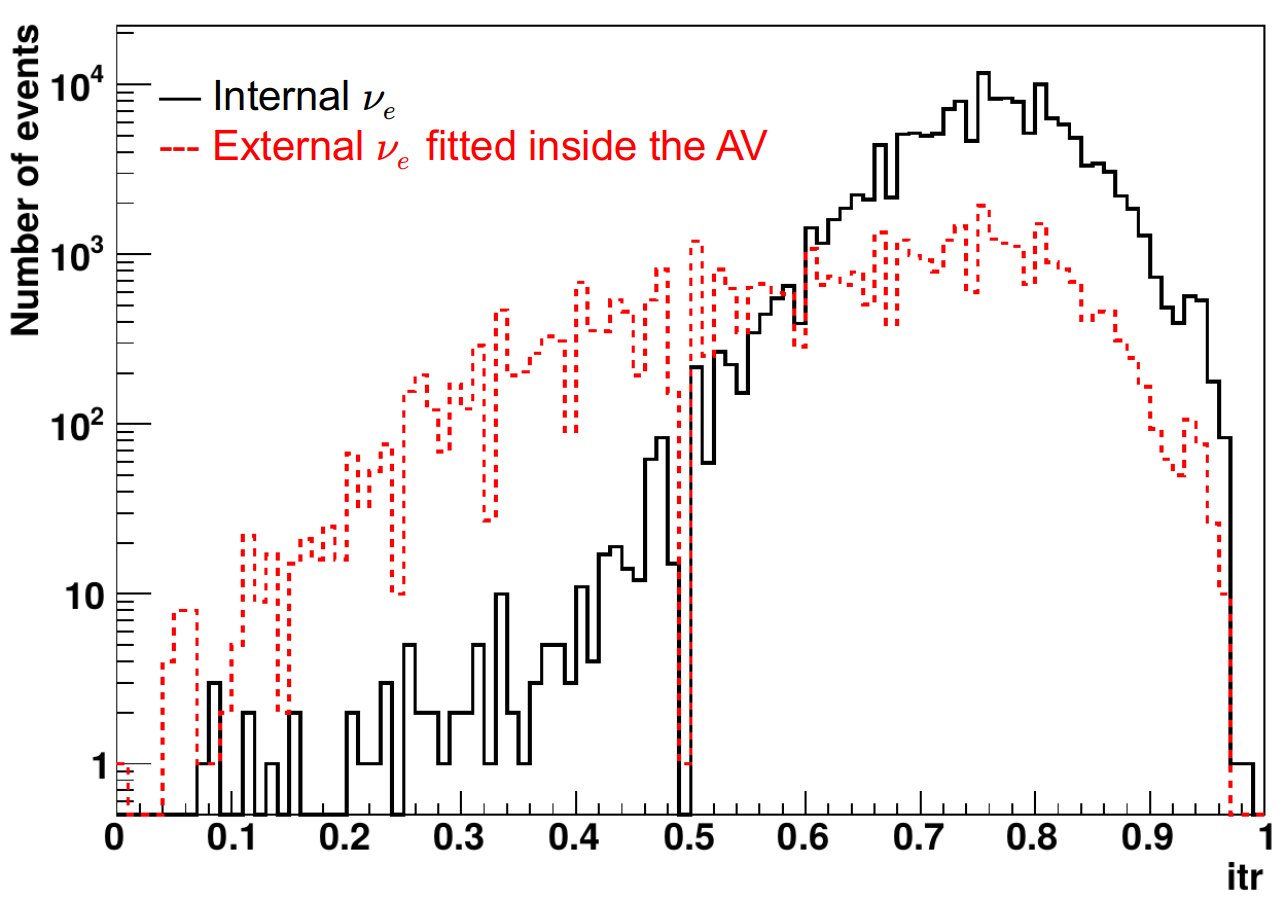
\includegraphics[width=8cm]{ITR_MPW_solarNuVsExSolar.png}
%	\caption{Comparison between solar $\nu_e$ and external solar $\nu_e$; MPW results.}
%	\label{itrCmp}
%\end{figure}
\subsubsection{TMVA Outputs for Data}

Fig.~\ref{cosThetaToSun_4to15_BDT} and Fig.~\ref{cosThetaToSun_5to15_BDT} show the BDT selection outputs from the 190.33-day dataset. Fig.~\ref{cosThetaToSun_4to15_MLP} and Fig.~\ref{cosThetaToSun_5to15_MLP} show the MLP outputs. 
Table.~\ref{table:eventNumbers} shows the number of the output events for different energy regions and from different methods.

Cuts on the position and energy FOMs suggested by the collaboration\cite{morganFOM} are \footnote{There is also a suggested cut on the quantity of $position_error$ ($position_error<525~mm$). However, since this quantity was not calculated by the MPW fitter, it was not included here.}: $-11<Z_{factor}<1$, $scaleLogL>10.85$, $0<G_{test}<1.9$, $U_{test}<0.95$, $ITR>0.55$, $-0.12<\beta_{14}<0.95$. Combined with the ``beforehand cuts'', the whole set of cuts is considered as ``default cuts'' here and is compared with the TMVA outputs.

%\begin{table}[ht]
%	\centering
%	\caption{Number of candidate events for different selection methods.}
%	\label{table:eventNumbers}
%	\begin{tabular*}{150mm}{c@{\extracolsep{\fill}}cccc}
%		\toprule
%		Method & selected signals ($S$) & backgrounds ($N$)& $S/N$ \\
%		\hline  %1472
%		$[4,15]~MeV$ & (total: 1922 events)& &\\
%		\hline
%		BDT & 367  & 1555 &0.236 \\
%		MLP & 484 & 1438 & 0.337\\
%		default cut &932   & 990& 0.941\\
%		\hline
%		$[5,15]~MeV$ & (total: 207 events)&  & \\
%		\hline
%		BDT & 156  & 51 & 3.06\\
%		MLP &  160 & 47 & 3.40 \\
%		default cut & 162 & 45 & 3.60\\
%		\bottomrule
%	\end{tabular*}
%\end{table}
%

\begin{figure}[!htb]
	\centering
	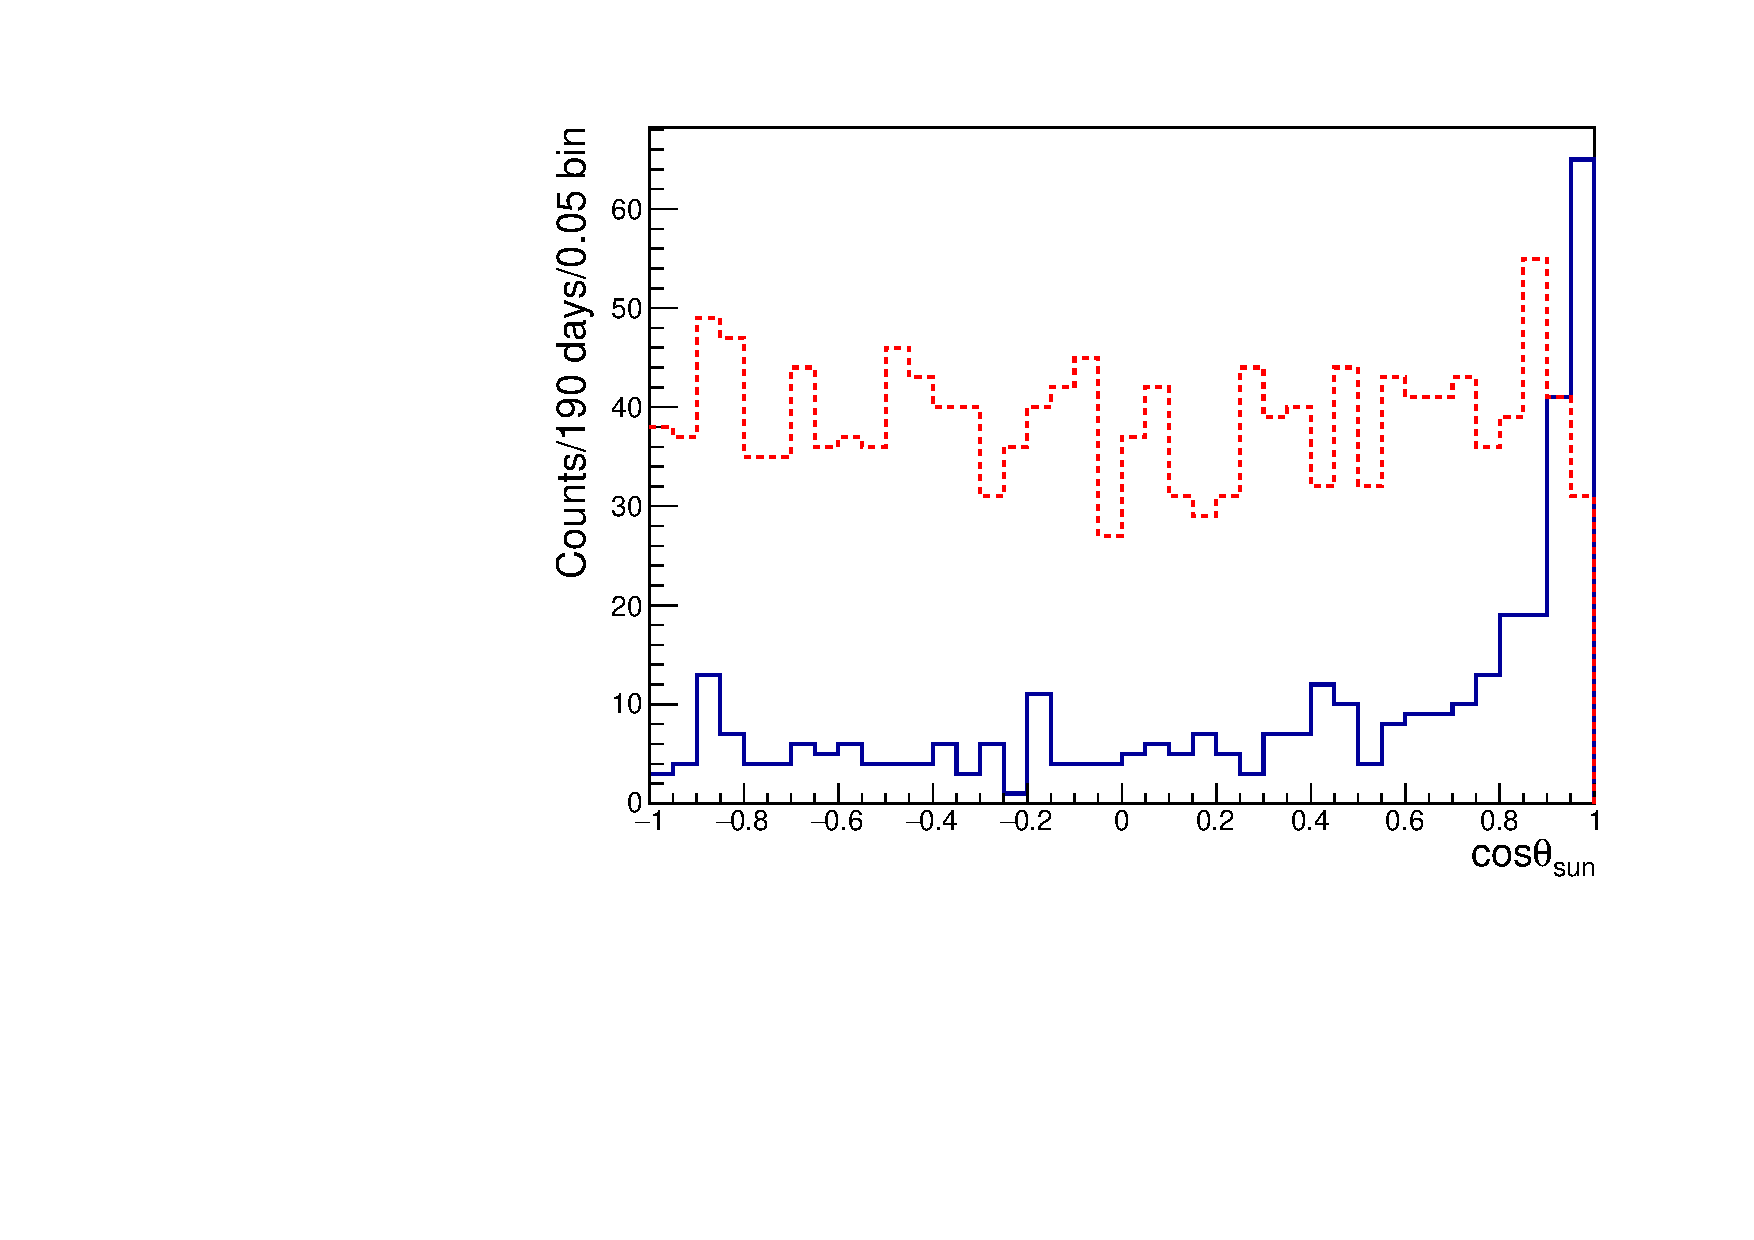
\includegraphics[width=8cm]{cosThetaToSun_4to15_BDT.pdf}
	\caption{BDT output for $\cos\theta_{sun}$, with $4<E_{fit}<15~MeV$. The solid blue line shows the selected candidate solar $\nu_e$ events while the dotted red line shows the selected background events.}
	\label{cosThetaToSun_4to15_BDT}
\end{figure}

\begin{figure}[!htb]
	\centering
	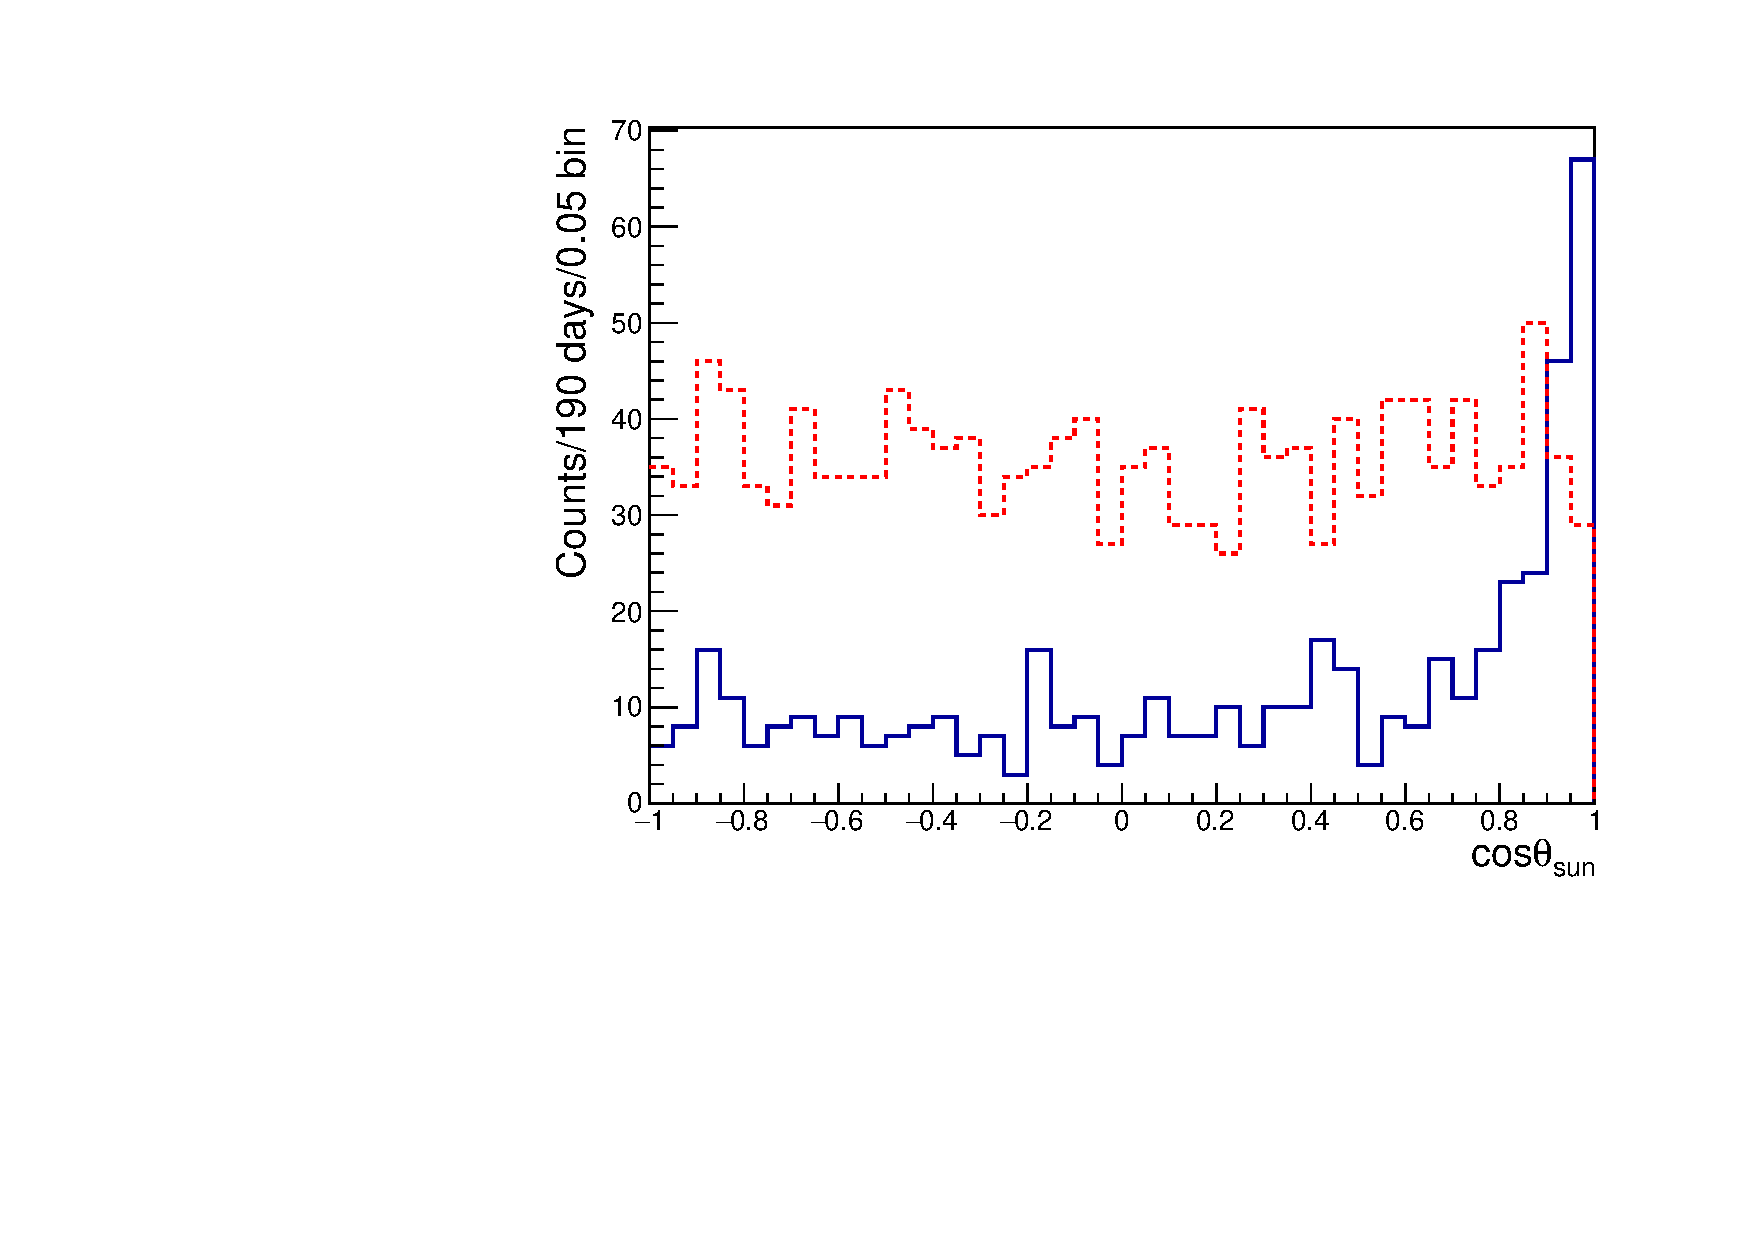
\includegraphics[width=8cm]{cosThetaToSun_4to15_MLP.pdf}
	\caption{MLP output for $\cos\theta_{sun}$, with $4<E_{fit}<15~MeV$. The solid blue line shows the selected candidate solar $\nu_e$ events while the dotted red line shows the selected background events.}
	\label{cosThetaToSun_4to15_MLP}
\end{figure}

\begin{figure}[!htb]
	\centering
	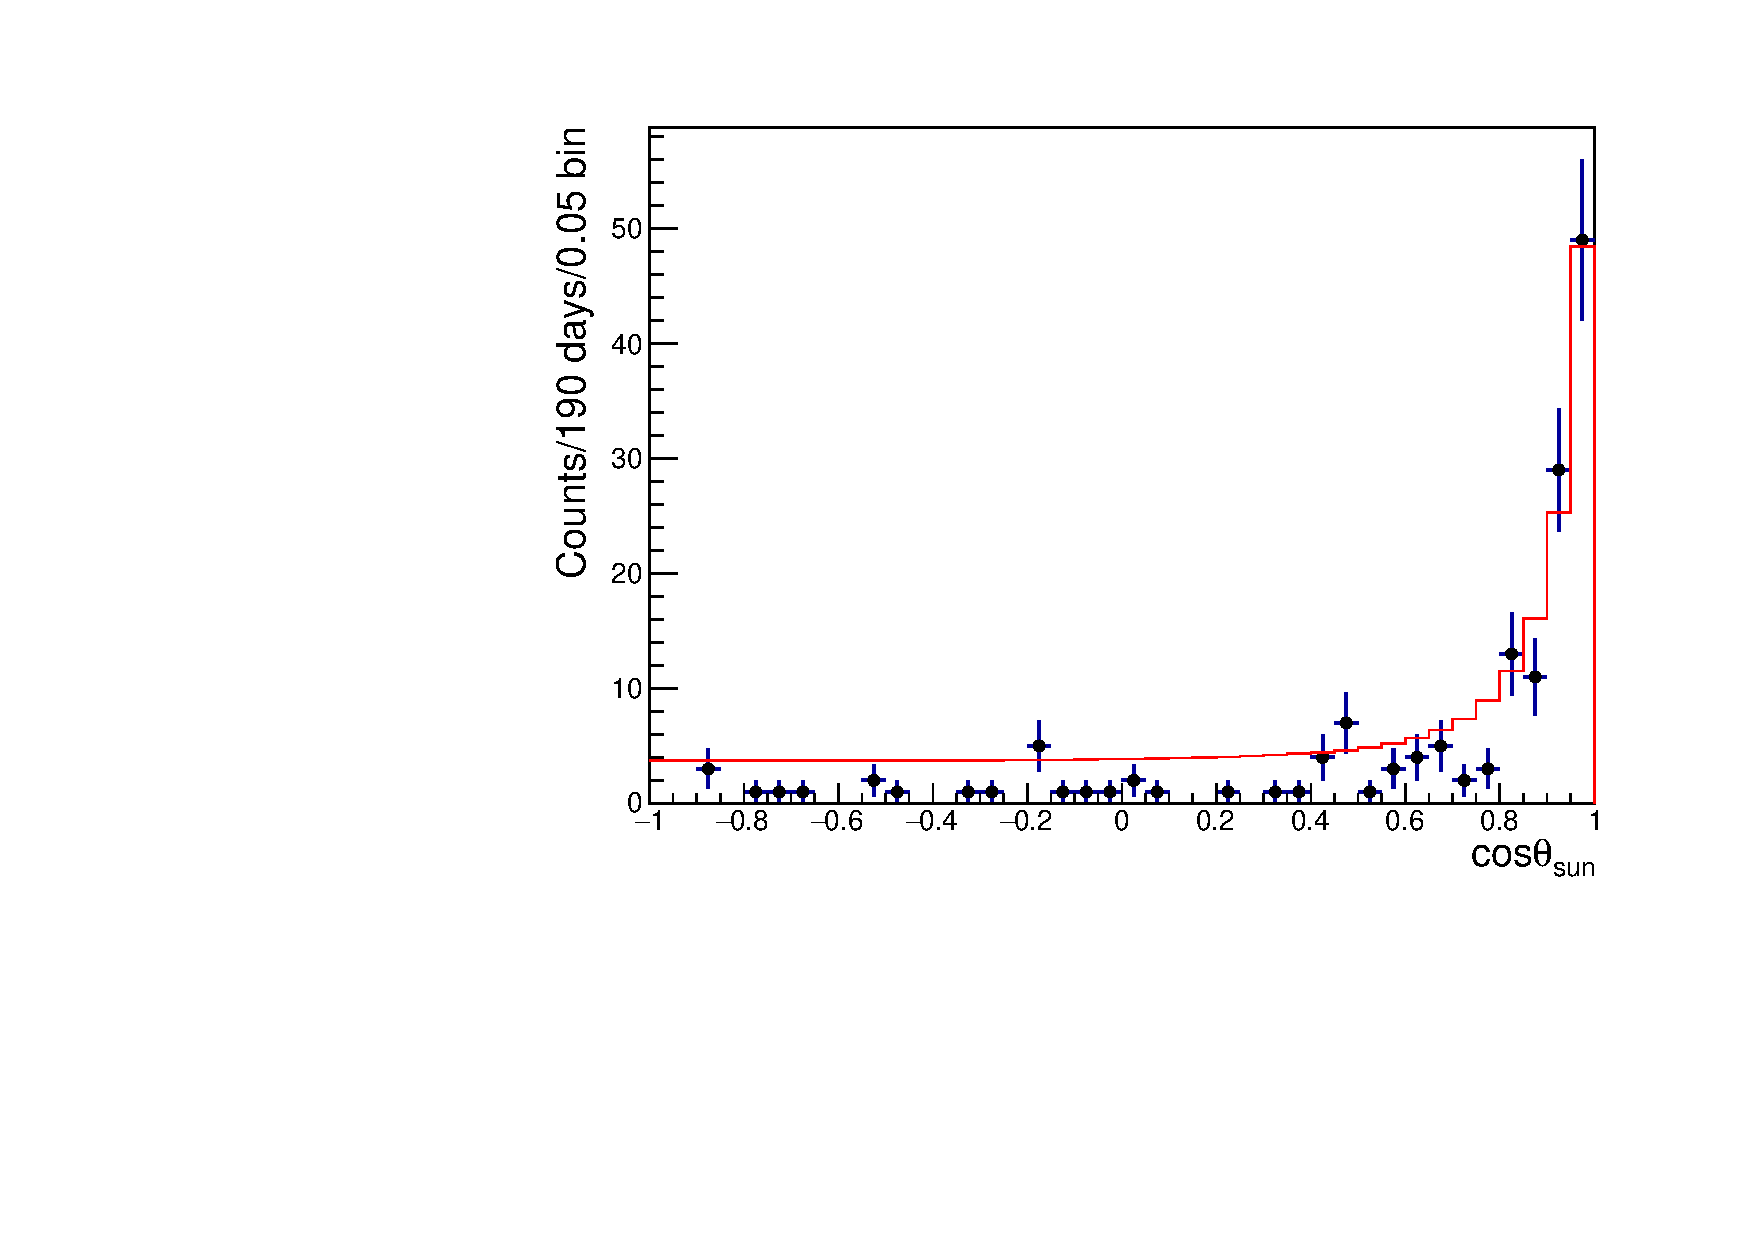
\includegraphics[width=8cm]{cosThetaToSun_5to15_BDT.pdf}
	\caption{BDT output for $\cos\theta_{sun}$, with $4<E_{fit}<15~MeV$. The solid blue line shows the selected candidate solar $\nu_e$ events while the dotted red line shows the selected background events.}
	\label{cosThetaToSun_5to15_BDT}
\end{figure}

\begin{figure}[!htb]
	\centering
	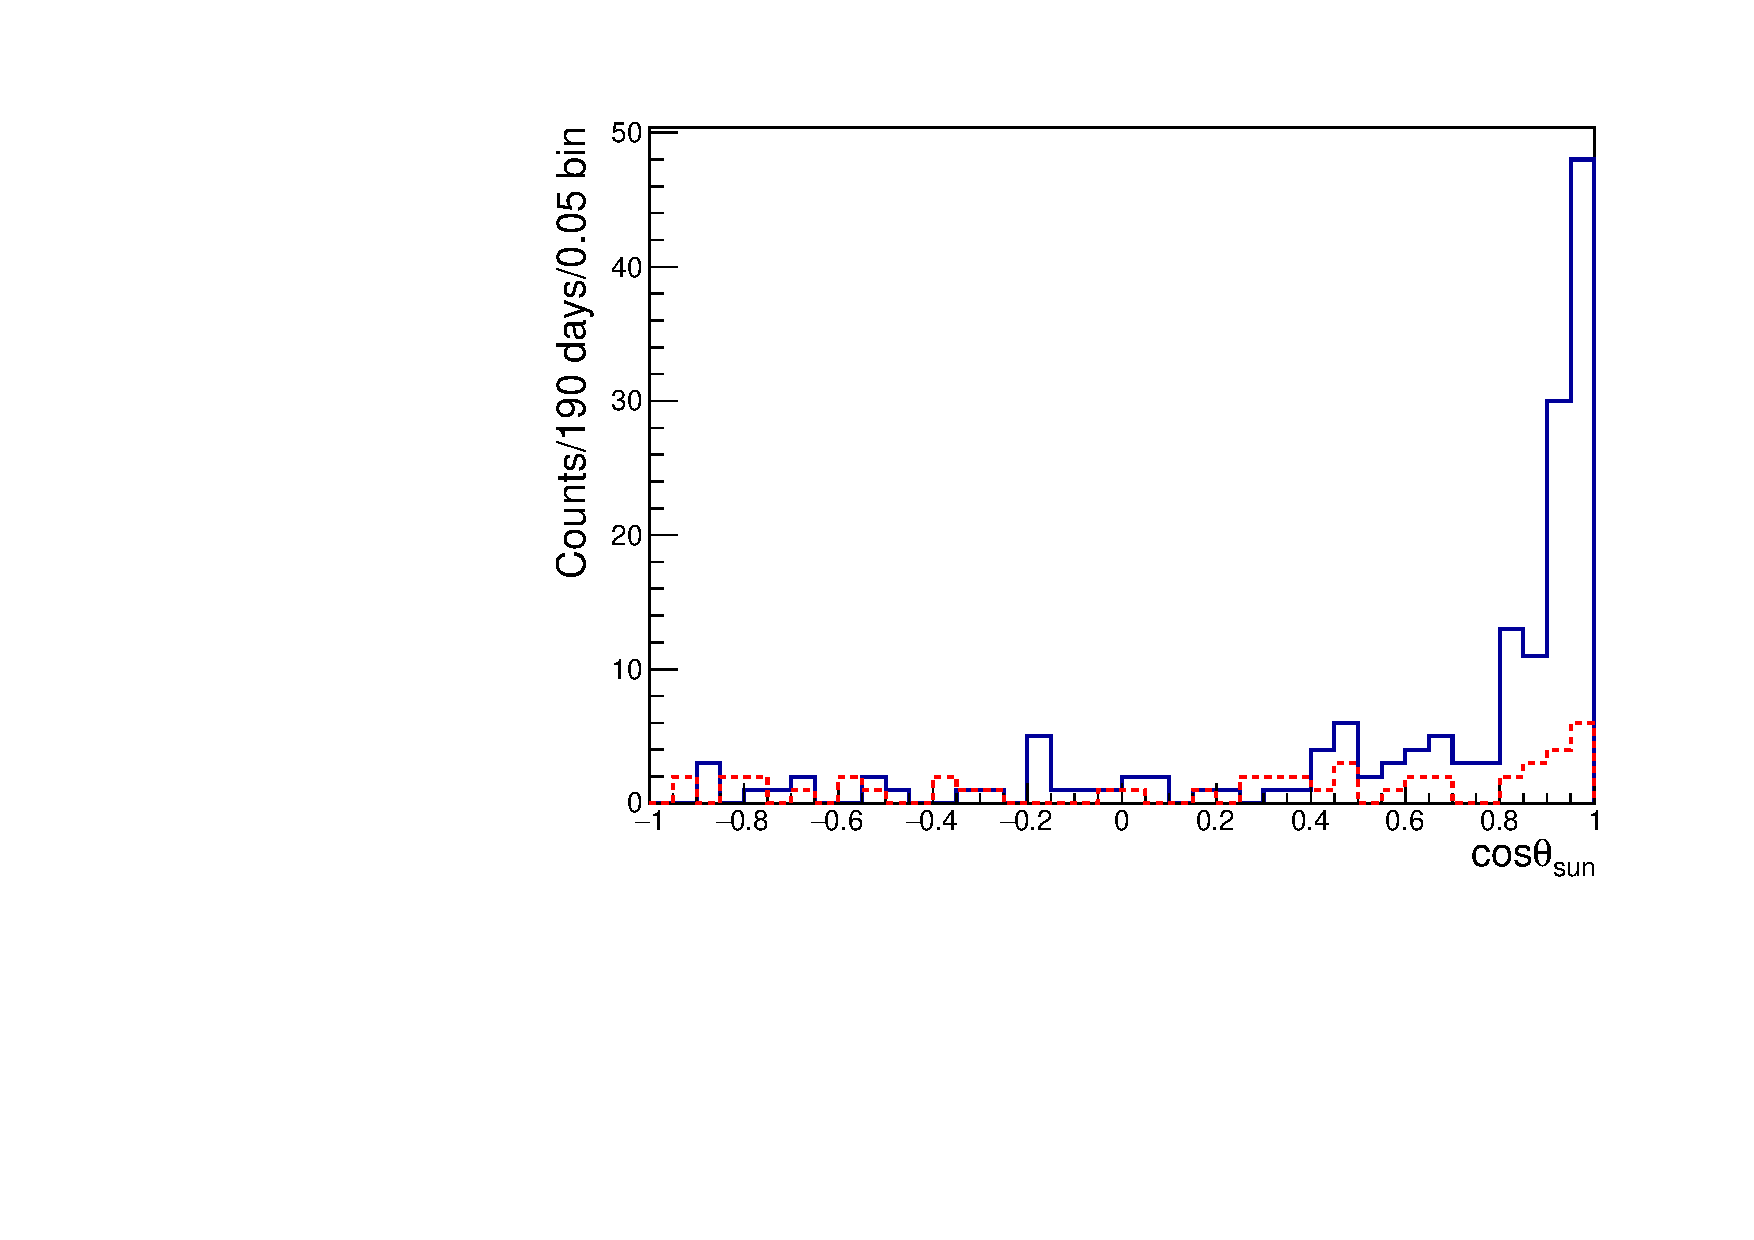
\includegraphics[width=8cm]{cosThetaToSun_5to15_MLP.pdf}
	\caption{MLP output for $\cos\theta_{sun}$, with $5<E_{fit}<15~MeV$. The solid blue line shows the selected candidate solar $\nu_e$ events while the dotted red line shows the selected background events.}
	\label{cosThetaToSun_5to15_MLP}
\end{figure}

%6<E_{fit}<15~MeV$

%Comparisons

The main analysis is focused on the [5,15] MeV energy region. A comparison of the outputs of $5<E_{fit}<15~MeV$ from the BDT, MLP and the default cuts is shown in Fig.~\ref{compare_cosThetaToSun_5to15}.
\begin{figure}[!htb]
	\centering
	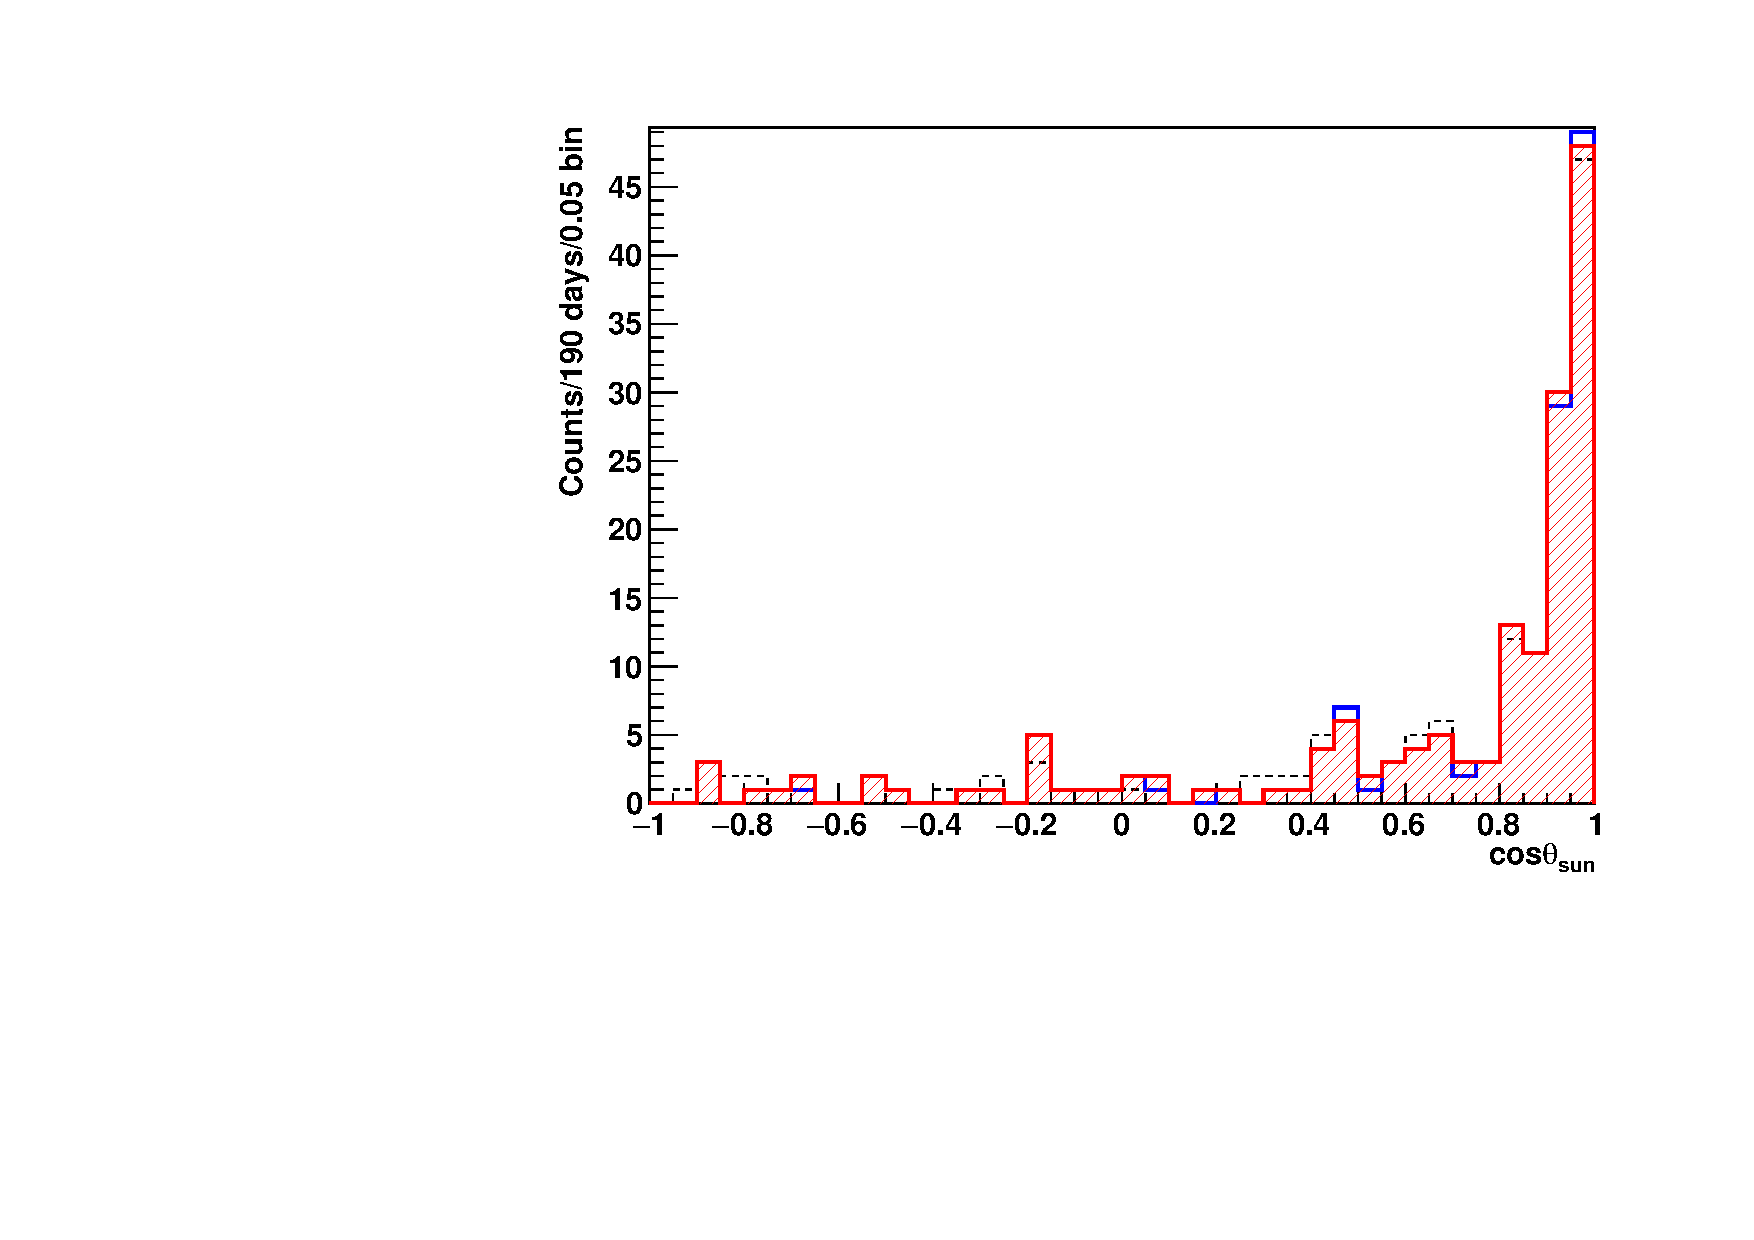
\includegraphics[width=8cm]{Compare_cosThetaSun_5to15.pdf}
	\caption{For the $5<E_{fit}<15~MeV$, comparing the outputs of the BDT, MLP and the default cuts. The solid blue line shows the BDT results; the red slashes show the MLP results and the dotted black line shows the default cut results.}
	\label{compare_cosThetaToSun_5to15}
\end{figure}

\subsection{Discussions on the TMVA Results}
A more stringent radial cut (or tighter FV) can be applied on lower energy region $4<E_{fit}<5~MeV$ to further remove the backgrounds which are dominant in lower energy region. However, this tighter cut can also reduce the number of signals.

Other packages developed for high energy particle physics, such as StatPatternRecognition (SPR)\cite{sprWebsite}, can also be considered as an alternative tool or as a reference for results comparisons. 

\subsection{Likelihood Fits for Solar Neutrino Candidate Events}
In the previous section, the optimized cuts obtained from the TMVA analysis were applied on the dataset. 

After the event selections, a distribution of $\cos\theta_{sun}$ extracted from the solar $\nu_e$ candidate events was obtained. 

\subsubsection{Maximum Likelihood Fit}\label{poisson_fit}
A maximum likelihood method was applied on the distribution to extract the number of the solar $\nu_e$ interaction events ($N_{sig}$) as well as the number of the background events ($N_{bkg}$).

The values of $\cos\theta_{sun}$ from the selected events were filled into a histogram divided into bins.
For each bin, the observed event number ($n_{obs}$) was considered as a sum of solar $\nu_e$ and background events. The $n_{obs}$ in each bin was assumed to follow a Poisson distribution: $Poisson(n_{obs}, N_{bkg}\cdot P_{bkg}+N_{sig}\cdot P_{ES}(E))$, where $P_{bkg}$ and $P_{ES}(E)$ are the assumed distribution of backgrounds and solar $\nu_e$ events respectively.

For the background events, a uniform distribution of $\cos\theta_{sun}$ was assumed. On the other hand, the $\cos\theta_{sun}$ distributions of solar $\nu_e$ were extracted from the realistic run simulations after applying the optimized cuts, as shown in Fig.~\ref{solarPDF}. 

\begin{figure}[!htb]
	\centering
	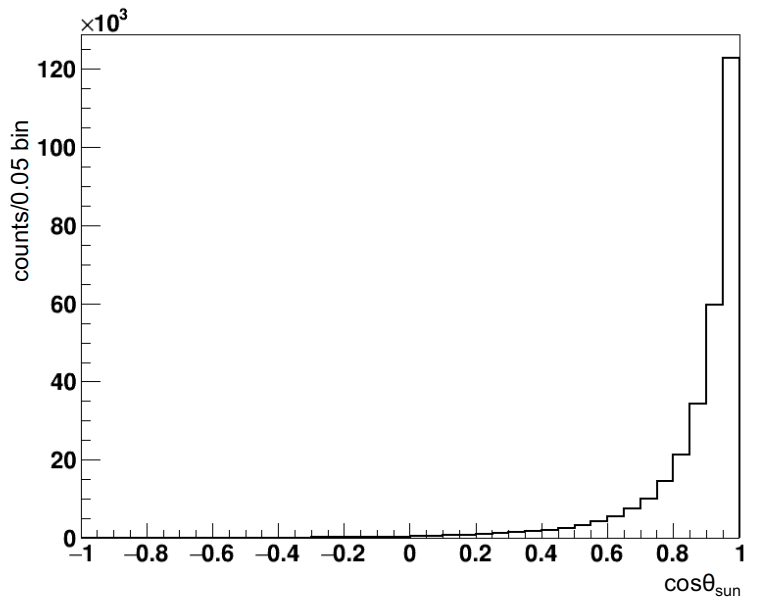
\includegraphics[width=10cm]{solarPDF.png}
	\caption{The $\cos\theta_{sun}$ distribution of solar $\nu_e$ extracted from the simulations, which was used as a pdf function.}
	\label{solarPDF}
\end{figure}

Adding up each bin $i$ and taking $N_{bkg}$ and $N_{sig}$ as the free parameters for fitting, the maximum likelihood function was built as\cite{pdg2020}:
%\begin{equation}\label{eq:solar_poissonFit}
%-\ln\mathcal L(N_{sig},N_{bkg}|n_{obs})
%=-\sum_i^{N_{bins}}\ln(Poisson(n^i_{obs}, N_{bkg}P^i_{bkg}+N_{sig}P^i_{ES}(E^i))).
%\end{equation}

\begin{equation}\label{eq:solar_poissonFitMinimizer}
-2\ln\mathcal \lambda(N_{sig},N_{bkg})
=2\sum_{i=0}^{N_{bins}}[\mu_i(N_{sig},N_{bkg})-n_i+n_i\ln\frac{n_i}{\mu_i(N_{sig},N_{bkg})}],
\end{equation}
where $\mu_i(N_{sig},N_{bkg})$ is the expected number of events in each bin: $\mu_i(N_{sig},N_{bkg})=N_{sig}\cdot P^i_{ES}(E^i)+N_{bkg}\cdot1/N_{bins}$; $N_{bins}$ is the total number of the bins, usually taken as 40 (per 0.05 bins). This quantity also includes the cases when the bin contains zero ($n_i=0$).

Fitting the data with $(N_{bkg},N_{sig})$ by maximizing the quantity \ref{eq:solar_poissonFitMinimizer}, $N_{bkg}$ and $N_{sig}$ were obtained. In the next section, an ensemble test based on fake datasets was used for testing the fit results.
%Fig.~\ref{solarFits1} shows the fit results. The fitted number of solar $\nu_e$ events is $N_{sig} = 67.1\pm9.2$, which is equivalent to a rate of $1.04\pm 0.14~event/(day\cdot kiloton)$; while the fitted number of background events is $N_{sig} = 3.4\pm0.91$, which is equivalent to a rate of $0.05\pm 0.01 event/(day\cdot kiloton)$.
%
%\begin{figure}[!htb]
%	\centering
%	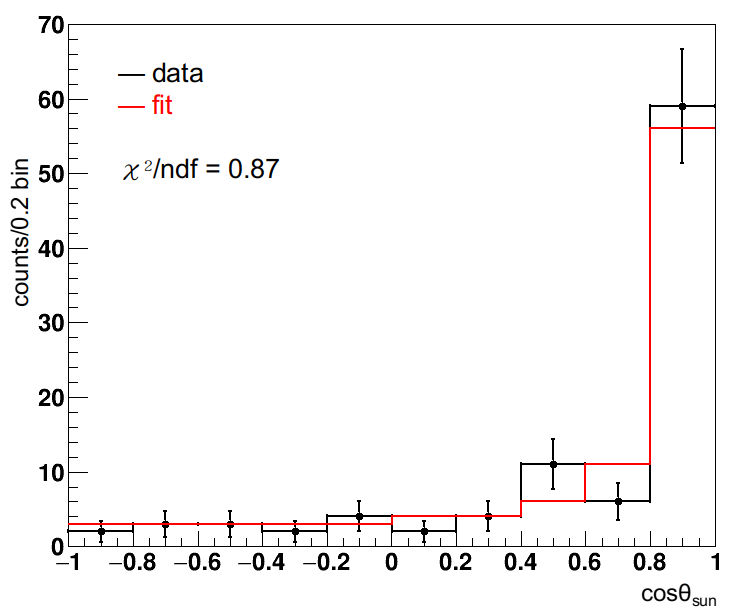
\includegraphics[width=8cm]{solarFits1.png}
%	\caption{Fitted results for the $N_{bkg}$ and $N_{sig}$ via the maximum likelihood method.}
%	\label{solarFits1}
%\end{figure}
%
%2D fits
\subsubsection{Ensemble Test}
To check the uncertainty of the Poisson fit, 5000 fake datasets were generated. Here I used the method similar to the \cite{leta}.
The fake data were taken from the MC simulation dataset of run-200004 to 203602 after the default cuts (the same to the one used by the TMVA). %In the MC dataset, for $E_{fit}>5~MeV$, there were 6359 backgrounds from different background events and 317205 signals of internal solar $\nu_e$ events (the event types were mentioned in Table.~\ref{table:mixed_MC}).

The number of backgrounds in a fake dataset, $N^f_{bkg}$, was assumed to be two times of the event number in the $-1<\cos\theta_{sun}<0$ region while the number of signals $N^f_{sig}=N^f_{total}-N^f_{bkg}$. Reading from the sub dataset of run-200004 to 203602 (see Fig.~\ref{half_data}), it found $N^f_{bkg}=38$ and then $N^f_{sig}=109-N^f_{bkg}=71$. To do the ensemble test, for each fake dataset, two random numbers: $N^r_{sig}$ and $N^r_{bkg}$ were generated by the $\texttt{ROOT TRandom3}$ random number generator class. Each of the two random numbers followed the random Poisson distribution: $e^{-\mu}\mu^{N^r}/N^r!$, where $\mu=71$ or $38$, and thus they fluctuated around $N^f_{sig}$ or $N^f_{bkg}$.

\begin{figure}[!htb]
	\centering
	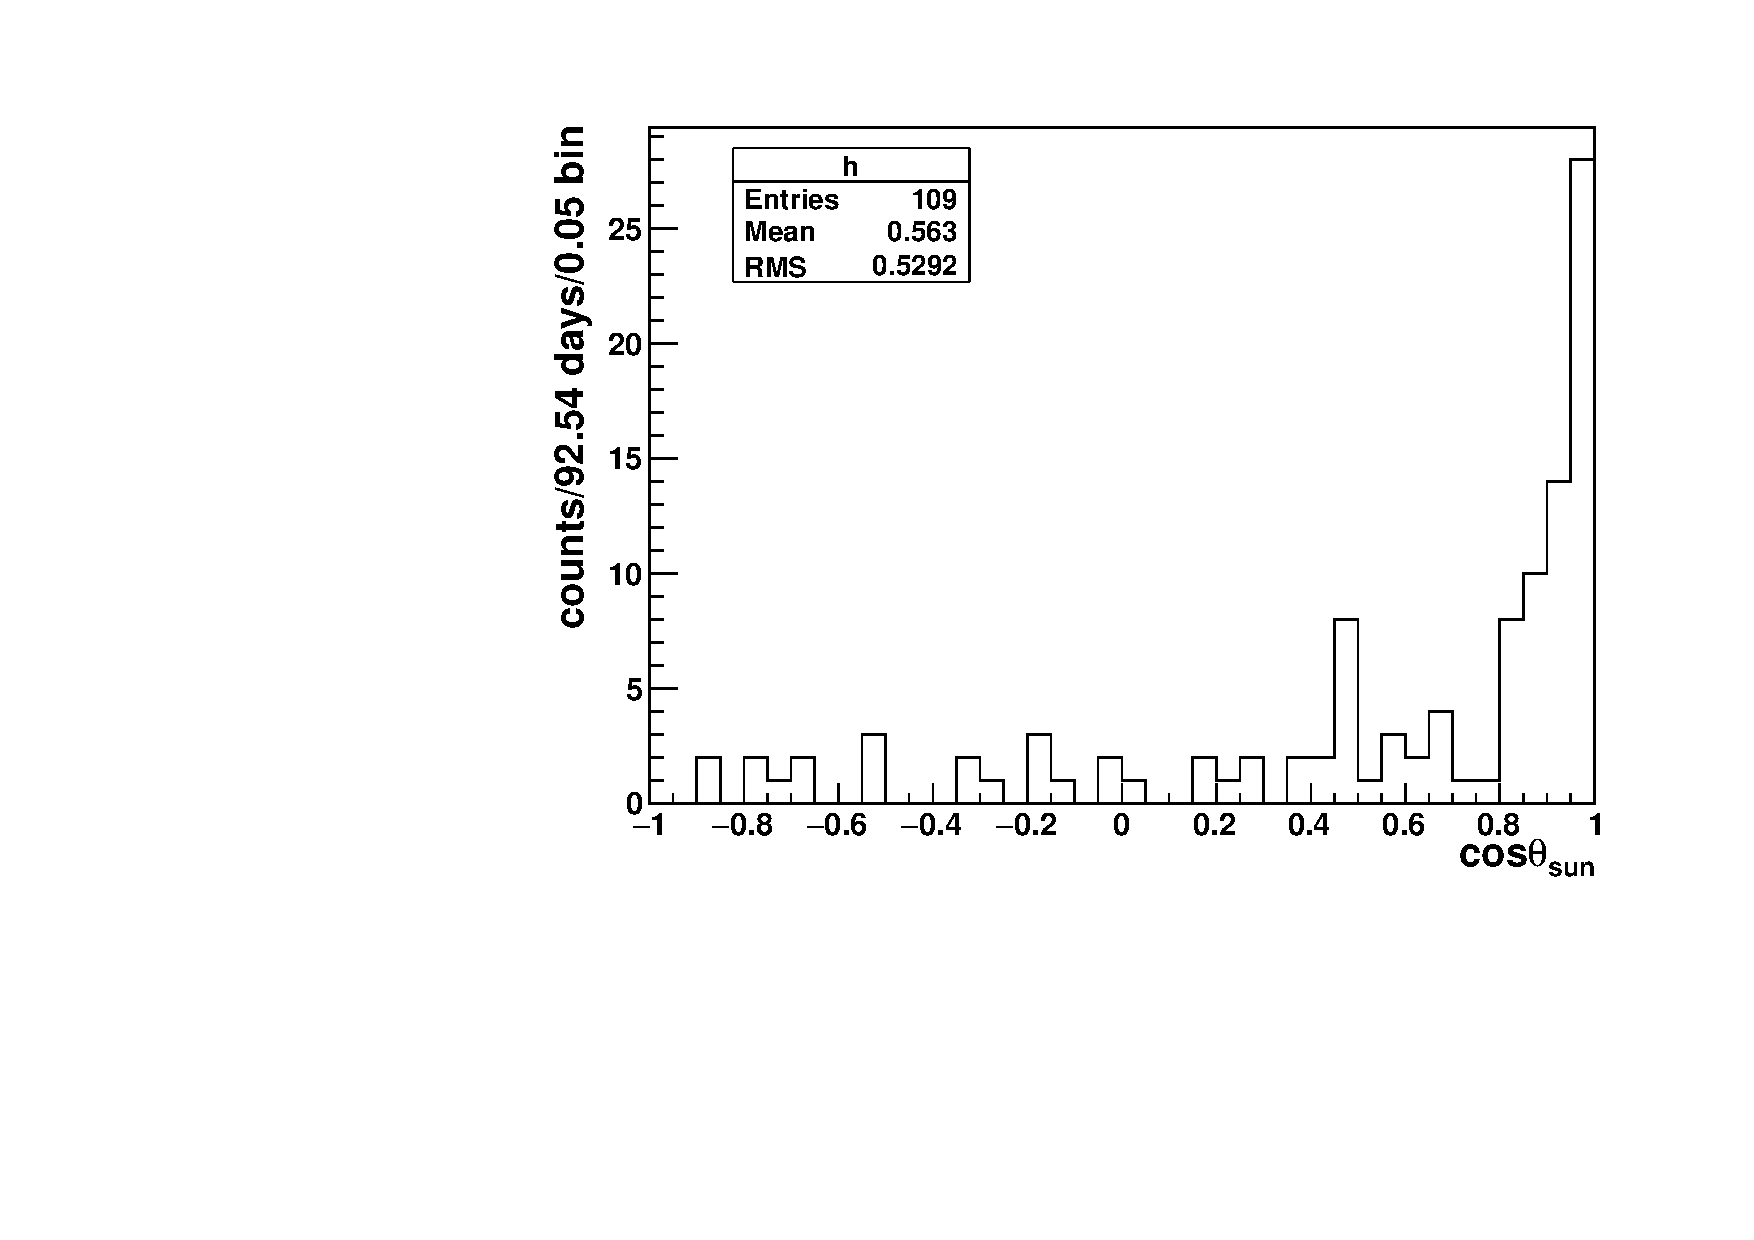
\includegraphics[width=10cm]{cosThetaToSun_halfData_5to15.pdf}
	\caption{Real data from run-200004 to 203602 (half dataset), after the default cuts. The number of counts in $-1<\cos\theta_{sun}<0$ region is 19.}
	\label{half_data}
\end{figure}

To create the fake datasets, $N^r_{sig}$ ($N^r_{bkg}$) events after the cuts were randomly and uniformly selected from the solar $\nu_e$ (merged backgrounds) MC simulations. For each randomly selected event, the values of $E_{fit}$ and $\cos\theta_{sun}$ were recorded. Each dataset was fitted with the maximum likelihood function described in \ref{poisson_fit}. Fig.~\ref{ensemble_test} shows an example of the fitted results.

\begin{figure}[!htb]
	\centering
	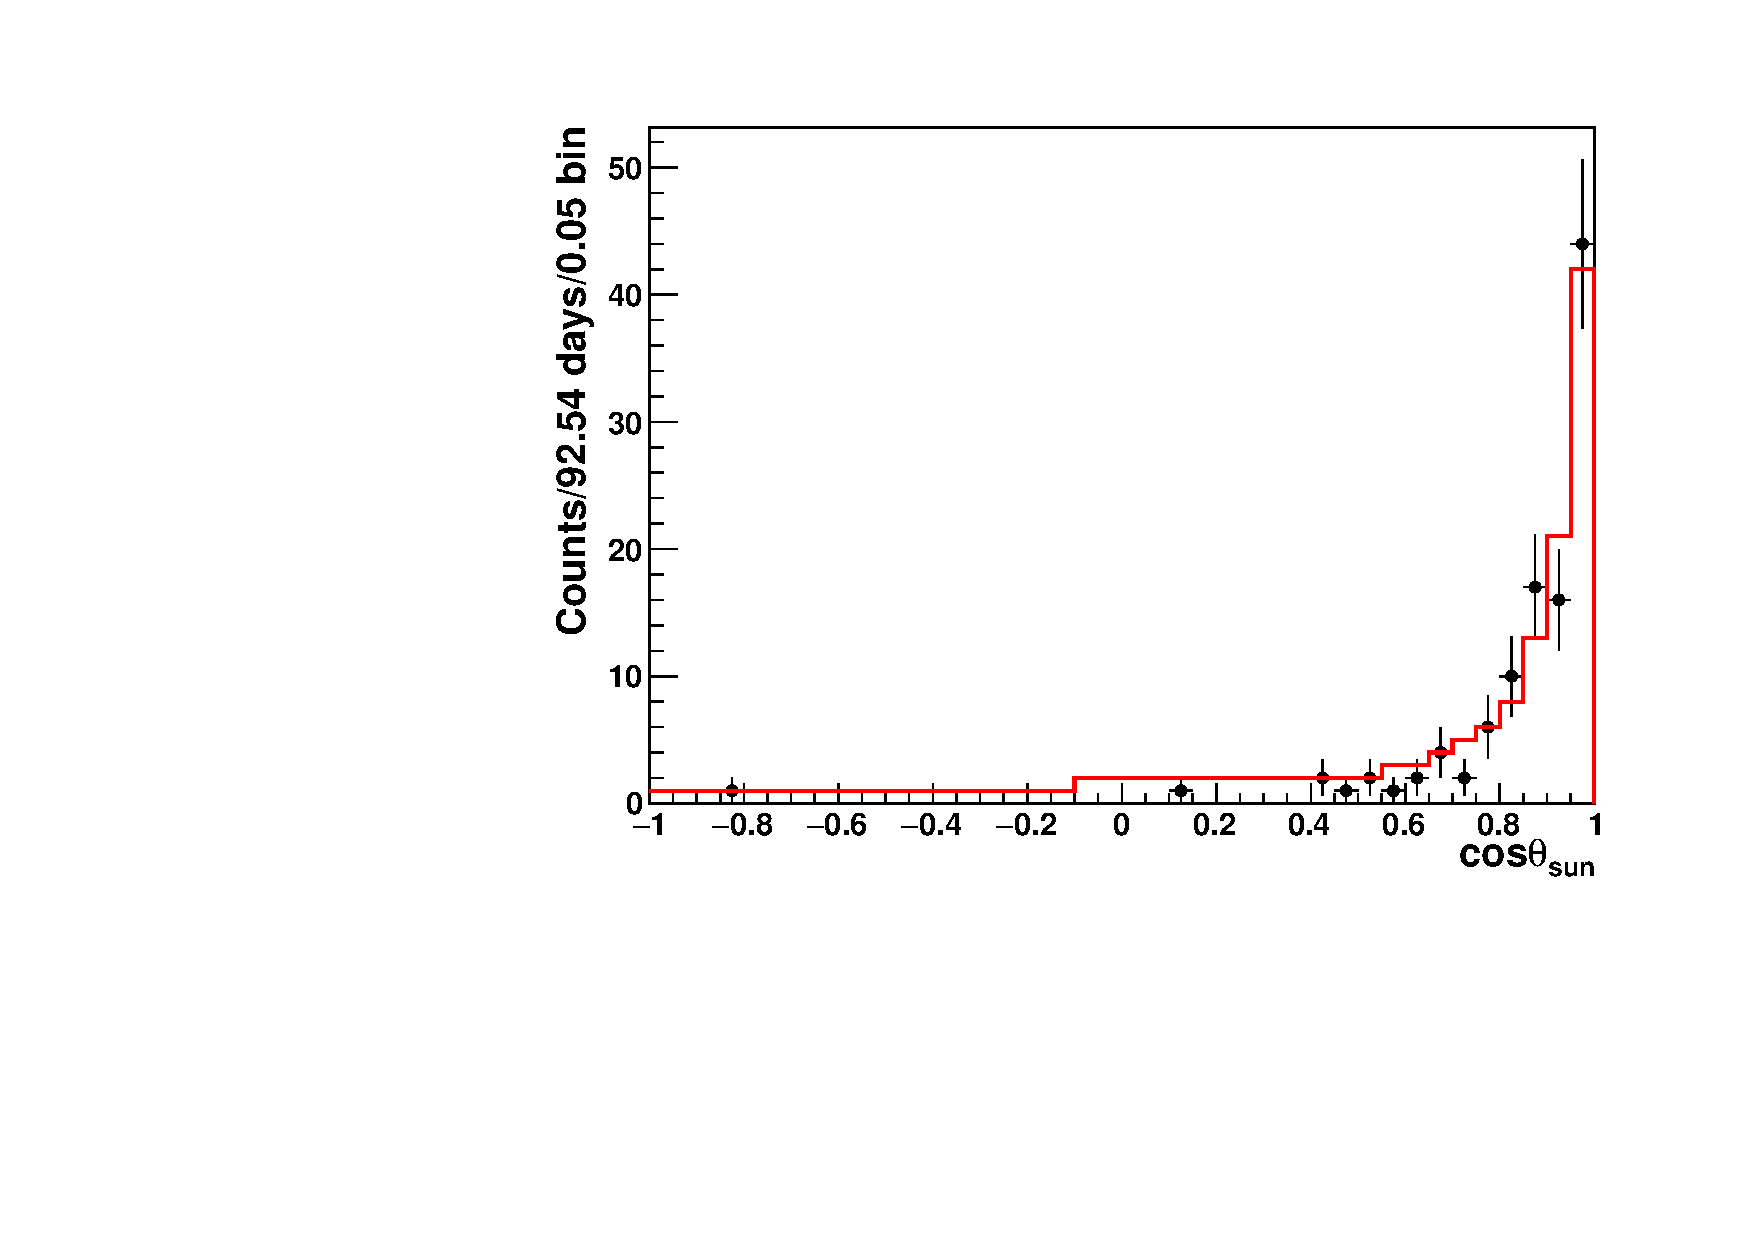
\includegraphics[width=10cm]{ensemble_fitExample.pdf}
	\caption{An example of the randomly generated $\cos\theta_{sun}$ fitted with $(N_{sig},N_{bkg})$. The black dots are data points and the red line is the fitted results. For $N^r_{sig} = 73$ and $N^r_{bkg}=44$, the fitted results give $N_{sig} = 73.42\pm9.42$ and $N_{bkg} = 43.58 \pm 7.73$, with a $\chi^2/ndf = 60.19/40 = 1.50$.}
	\label{ensemble_test}
\end{figure} 

The fit pull and the fit bias were defined by \cite{leta}:
\begin{equation}
bias=\frac{N_{sig}-N^r_{sig}}{N_{sig}},
\end{equation}

\begin{equation}
pull=\frac{N_{sig}-N^r_{sig}}{\sigma_{sig}},
\end{equation}
where $N_{sig}$ is the fitted number of signal events, $\sigma_{sig}$ is the statistical uncertainty of $N_{sig}$; $N^{r}_{sig}$ is used as the true number of signal events in the fake dataset.

Fig.~\ref{poisson_fitPull} and Fig.~\ref{poisson_fitBias} show the fit pull and biases respectively. The histograms were fitted with Gaussians. For the fitted number of signal events, the Gaussian mean of the fit biases is $-0.0044\pm0.0008$ for 5000 fake datasets while the Gaussian mean of the fit pulls is $-0.026\pm0.006$. These pulls and biases will be applied on the data. Fig.~\ref{poisson_fitLnL} shows the distributions of the $-2\ln L$ returned by the best fitted results ($-2\ln L_{best}$). The distribution, $f({-2\ln L_{best}})$, follows the asymptotic $\chi^2$ pdf with a degree of 40 and is used to compute the p-values\cite{pdg2020}. For a best-fit set ($N^i_{sig},N^i_{bkg}$) with a value of $-2\ln L^i_{best}$, the p-value is calculated as $p=\int_{-2\ln L^{i}_{best}}^{-2\ln L^{max}_{best}}f({-2\ln L_{best}})d(-2\ln L_{best})$.

\begin{figure}[!htb]
	\centering
	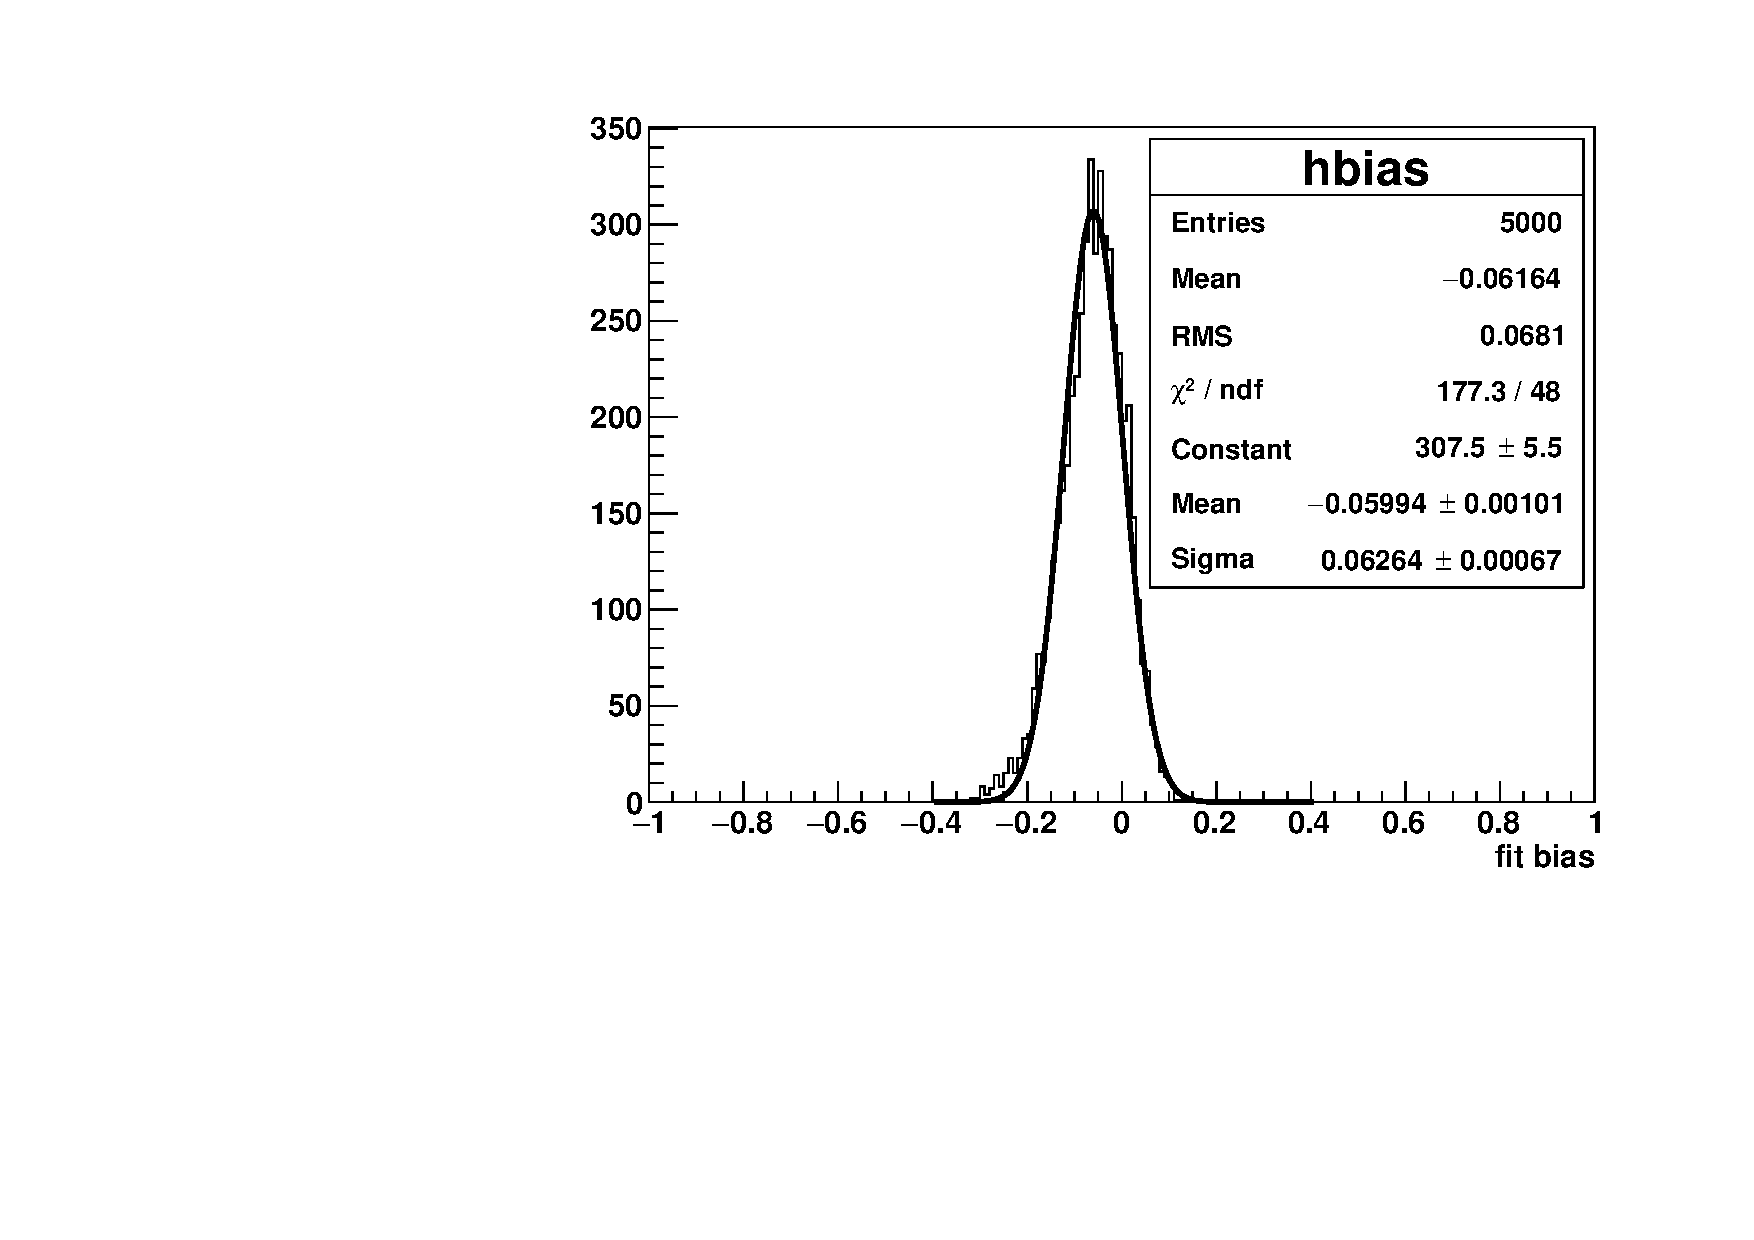
\includegraphics[width=8cm]{ensemble_fitBias.pdf}
	\caption{$N_{sig}$ fit biases for 5000 fake datasets.}
	\label{poisson_fitBias}
\end{figure} 

\begin{figure}[!htb]
	\centering
	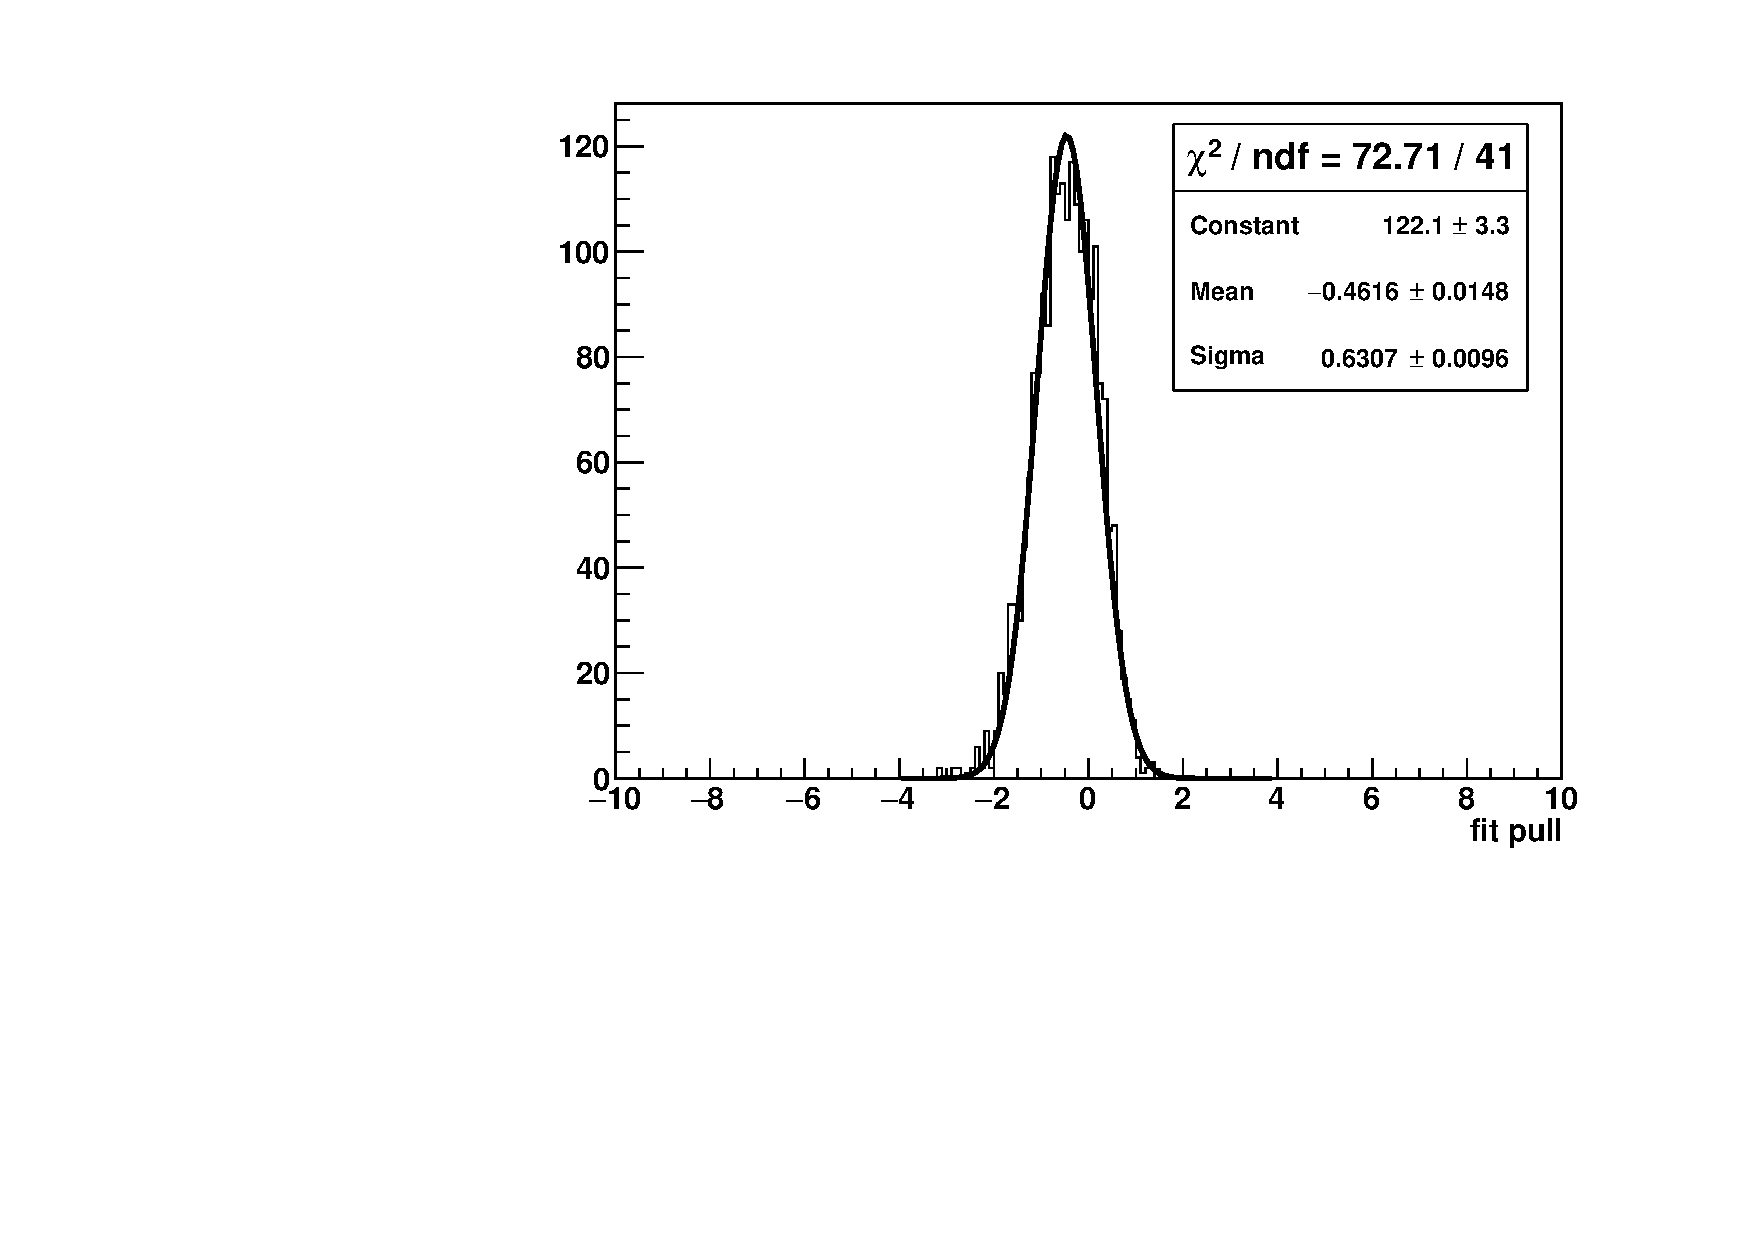
\includegraphics[width=8cm]{ensemble_fitPull.pdf}
	\caption{$N_{sig}$ fit pulls for 5000 fake datasets.}
	\label{poisson_fitPull}
\end{figure} 

\begin{figure}[!htb]
	\centering
	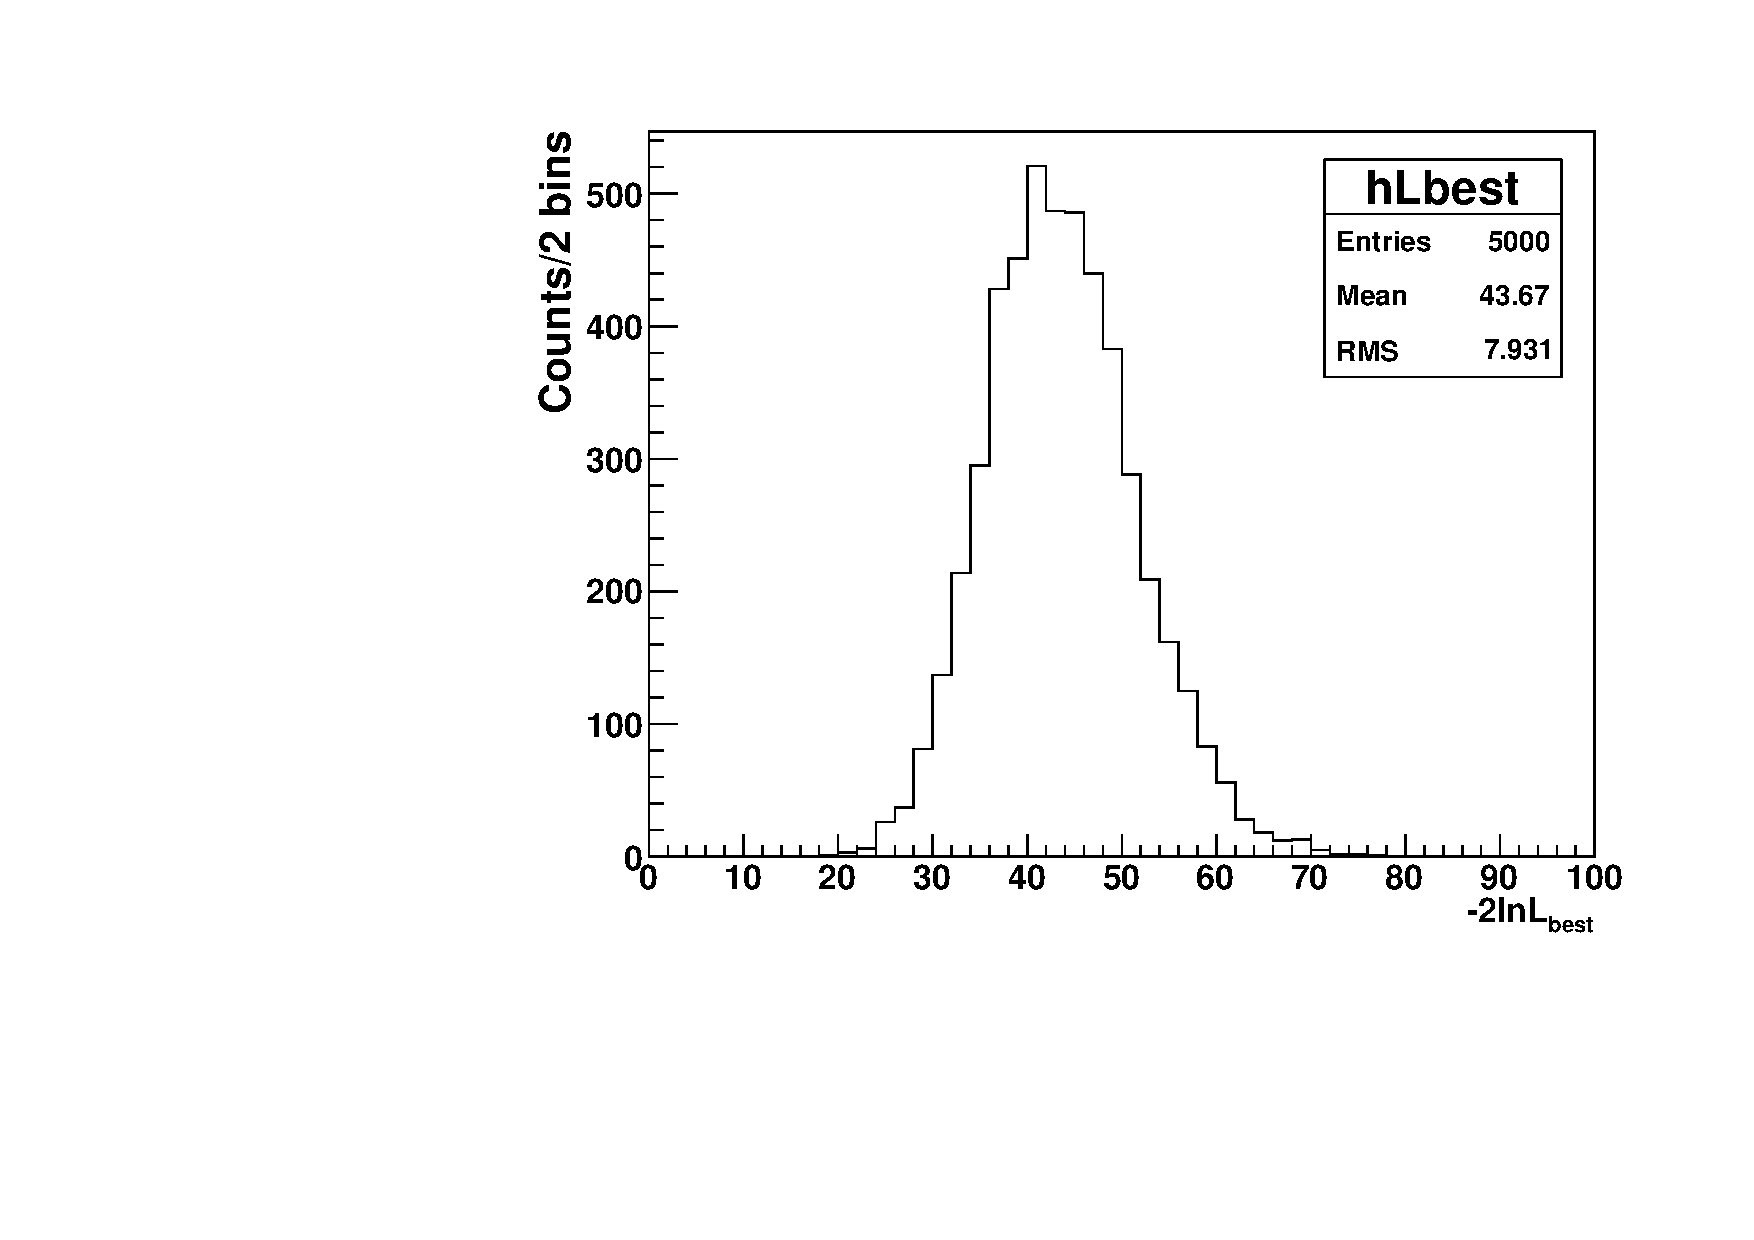
\includegraphics[width=8cm]{ensemble_lnLbest.pdf}
	\caption{The $-2\ln L$ of the best fitted results for 5000 fake datasets.}
	\label{poisson_fitLnL}
\end{figure}

\subsubsection{Fitting on the Whole Dataset (run-200004 to 207718)}
The whole dataset started from run-200004 (on 24 Oct, 2018) to run-207718 (on 10 July, 2019). This dataset has a live time of 190.33 days. The BDT and MLP were applied on this dataset.

In the region of $5<E_{fit}<15~MeV$, the outputs from the BDT and MLP were fitted to obtain the $N_{sig}$ and $N_{bkg}$. Fig.~\ref{wholeDataset_poissonFit_bdt} and Fig.~\ref{wholeDataset_poissonFit_mlp} show their results respectively.

These results are also summarized in Table.~\ref{table:wholedata_output}.

\begin{figure}[!htb]
	\centering
	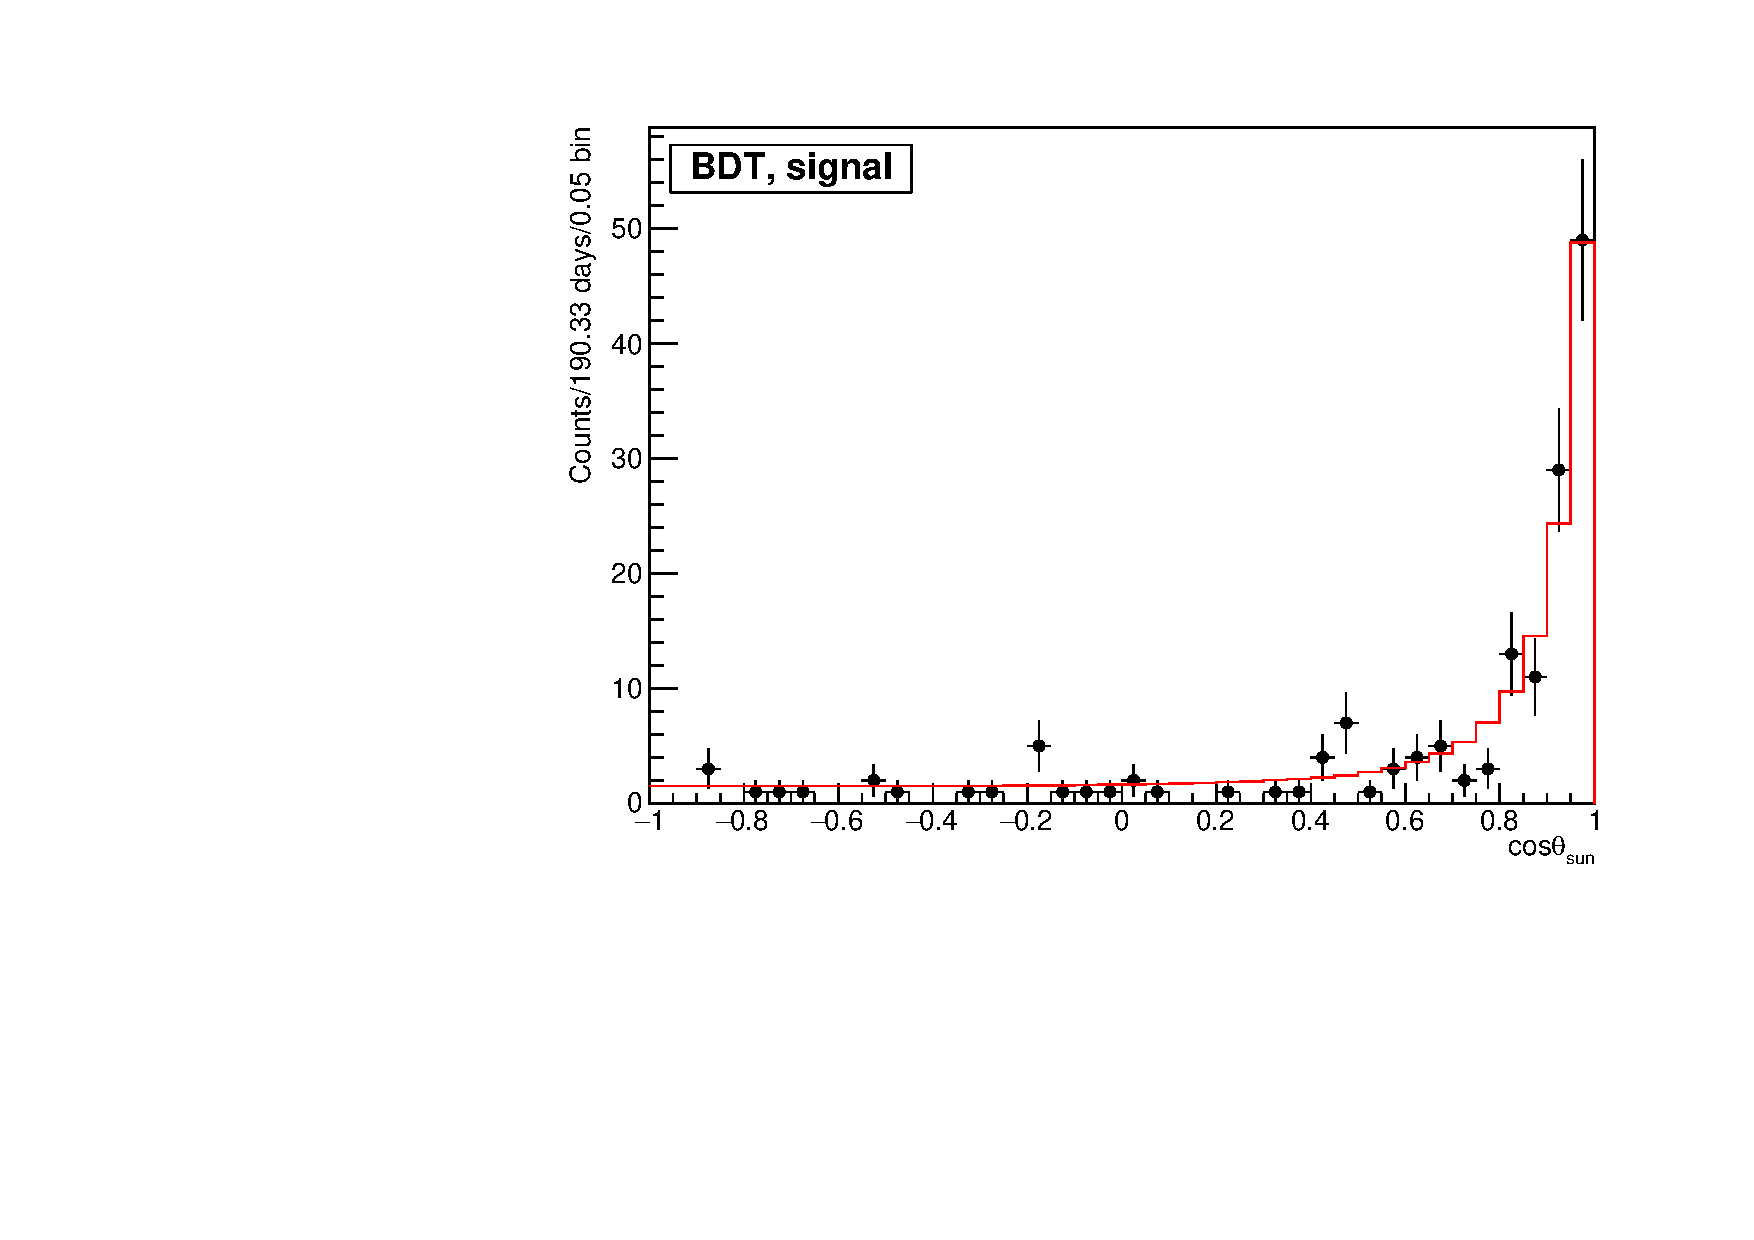
\includegraphics[width=10cm]{wholedataFit_bdt.pdf}
	\caption{Fitted results for the $5<E_{fit}<15~MeV$, from BDT outputs.} \label{wholeDataset_poissonFit_bdt}
\end{figure} 

\begin{figure}[!htb]
	\centering
	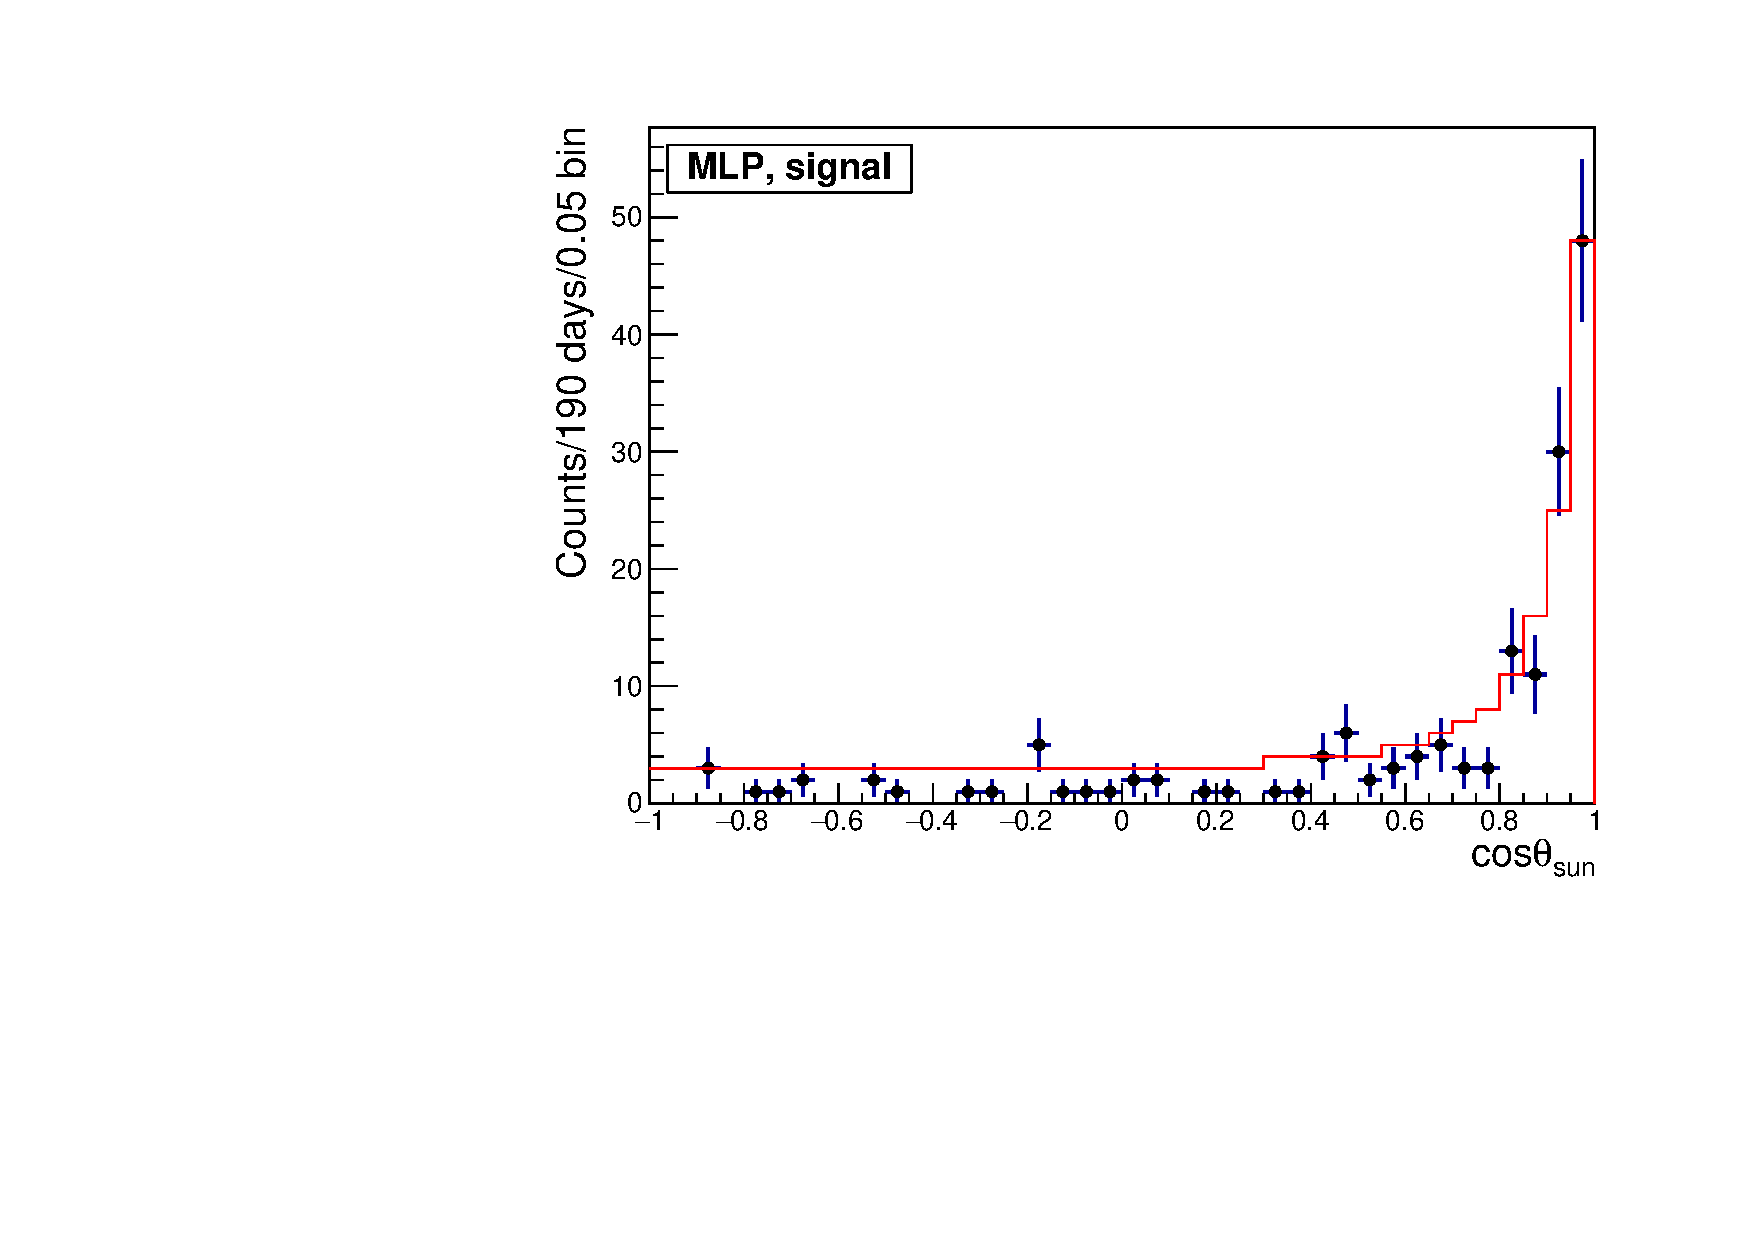
\includegraphics[width=10cm]{wholedataFit_mlp.pdf}
	\caption{Fitted results for the $5<E_{fit}<15~MeV$, from MLP outputs.}
	\label{wholeDataset_poissonFit_mlp}
\end{figure} 

\begin{table}[ht]
	\centering
	\caption{Fitted results for the whole dataset ($5<E<15~MeV$).}
	\label{table:wholedata_output}

	\begin{tabular*}{150mm}{c@{\extracolsep{\fill}}cccccc}
		\toprule
		Methods & $N_{sig}$ & $N_{bkg}$ & $R_{sig}$ & $R_{bkg}$ & p-value \\
		\hline
		BDT &$119.40\pm11.84$ & $36.55
\pm7.57$ & $0.90\pm0.09$ & $0.28\pm0.06$ & 0.07\\
		MLP &$119.49\pm11.89$ & $40.51\pm7.91$ & $0.90\pm0.09$  & $0.31\pm 0.06$  & 0.20\\
		%default cuts& \\ 
		\bottomrule
	\end{tabular*}
\end{table}

It can be concluded here that in the $[5,15]~MeV$ energy region, the BDT results are consistent with the MLP results. The estimated background rate is lower than the signal rate, which indicates that an extremely low background is achieved for the data.

\subsubsection{Systematics Evaluation}
The systematics of position, direction and energy reconstruction were obtained from the Chapter 5. The quantities of position scale ($XYZ_{scale}$), position resolution ($XYZ_{resol}$), direction resolution ($Dir_{resol}$), energy scale ($E_{scale}$) and energy resolution ($E_{resol}$) were used. Table.~\ref{table:solar_uncertainties} summarizes these quantities used for this analysis.

\begin{table}[ht]
	\centering
	\caption{Systematics for the solar $\nu_e$ analysis in the water phase.}
	\label{table:solar_uncertainties}
	\begin{tabular*}{80mm}{c@{\extracolsep{\fill}}cc}
		\toprule
		Systematics & values (positive/negative)\\
		\hline
		x shift & +6.48/-5.98 mm\\	
		y shift & +6.13/-4.11 mm\\
		z shift & +6.71/-4.82 mm\\
		x scale & +0.07\%/-0.06\%\\	
		y scale & +0.02\%/-0.07\%\\
		z scale & +0.08\%/-0.01\%\\
	    $\delta_\theta$  & +0.013/-0.101\\
	    $E_{scale}$ &  2.0\% \\
	    $E_{resol}$ &  0.011\\
	    $\beta_{14}$ shifts & +0.010/-0.036\\
		\bottomrule
	\end{tabular*}
\end{table}

%energy scale
For the energy scale, the reconstructed MC energies were scaled up and down the expected number of signal events, the uncertainty on the expected number of events was obtained to be $^{+0.05}_{-0.06}$.

%the energy resolution was determined to be $21.0^{+5.0}_{-9.2}\%$ at 5 MeV.

A remapping of $\cos\theta_{sun}$ by using the equation \ref{remapTheta} was applied on the spectrum for evaluating the systematics. a minus symbol should be applied, and it is found as:

\begin{equation}\label{remapThetaSun}
-\cos\theta_{sun}'=1+(-\cos\theta_{sun}-1)(1+\delta_{\theta}),
\end{equation} 

So the transformation then becomes: $\cos\theta_{sun}'=-1+(\cos\theta_{sun}+1)(1+\delta_{\theta})$.


Its impact is $^{+0.3}_{-0.2}$ events.





\subsubsection{Extracting the Solar Neutrino Flux}

live time scale: $\frac{t_{data~live~time}}{t_{MC~run~time}}=0.96$.







%Combine the $\nu_\mu$ MC spectrum with the $\nu_e$, as shown in Fig.~\ref{combine_numu_nue}.

%\begin{figure}[!htb]
%	\centering
%	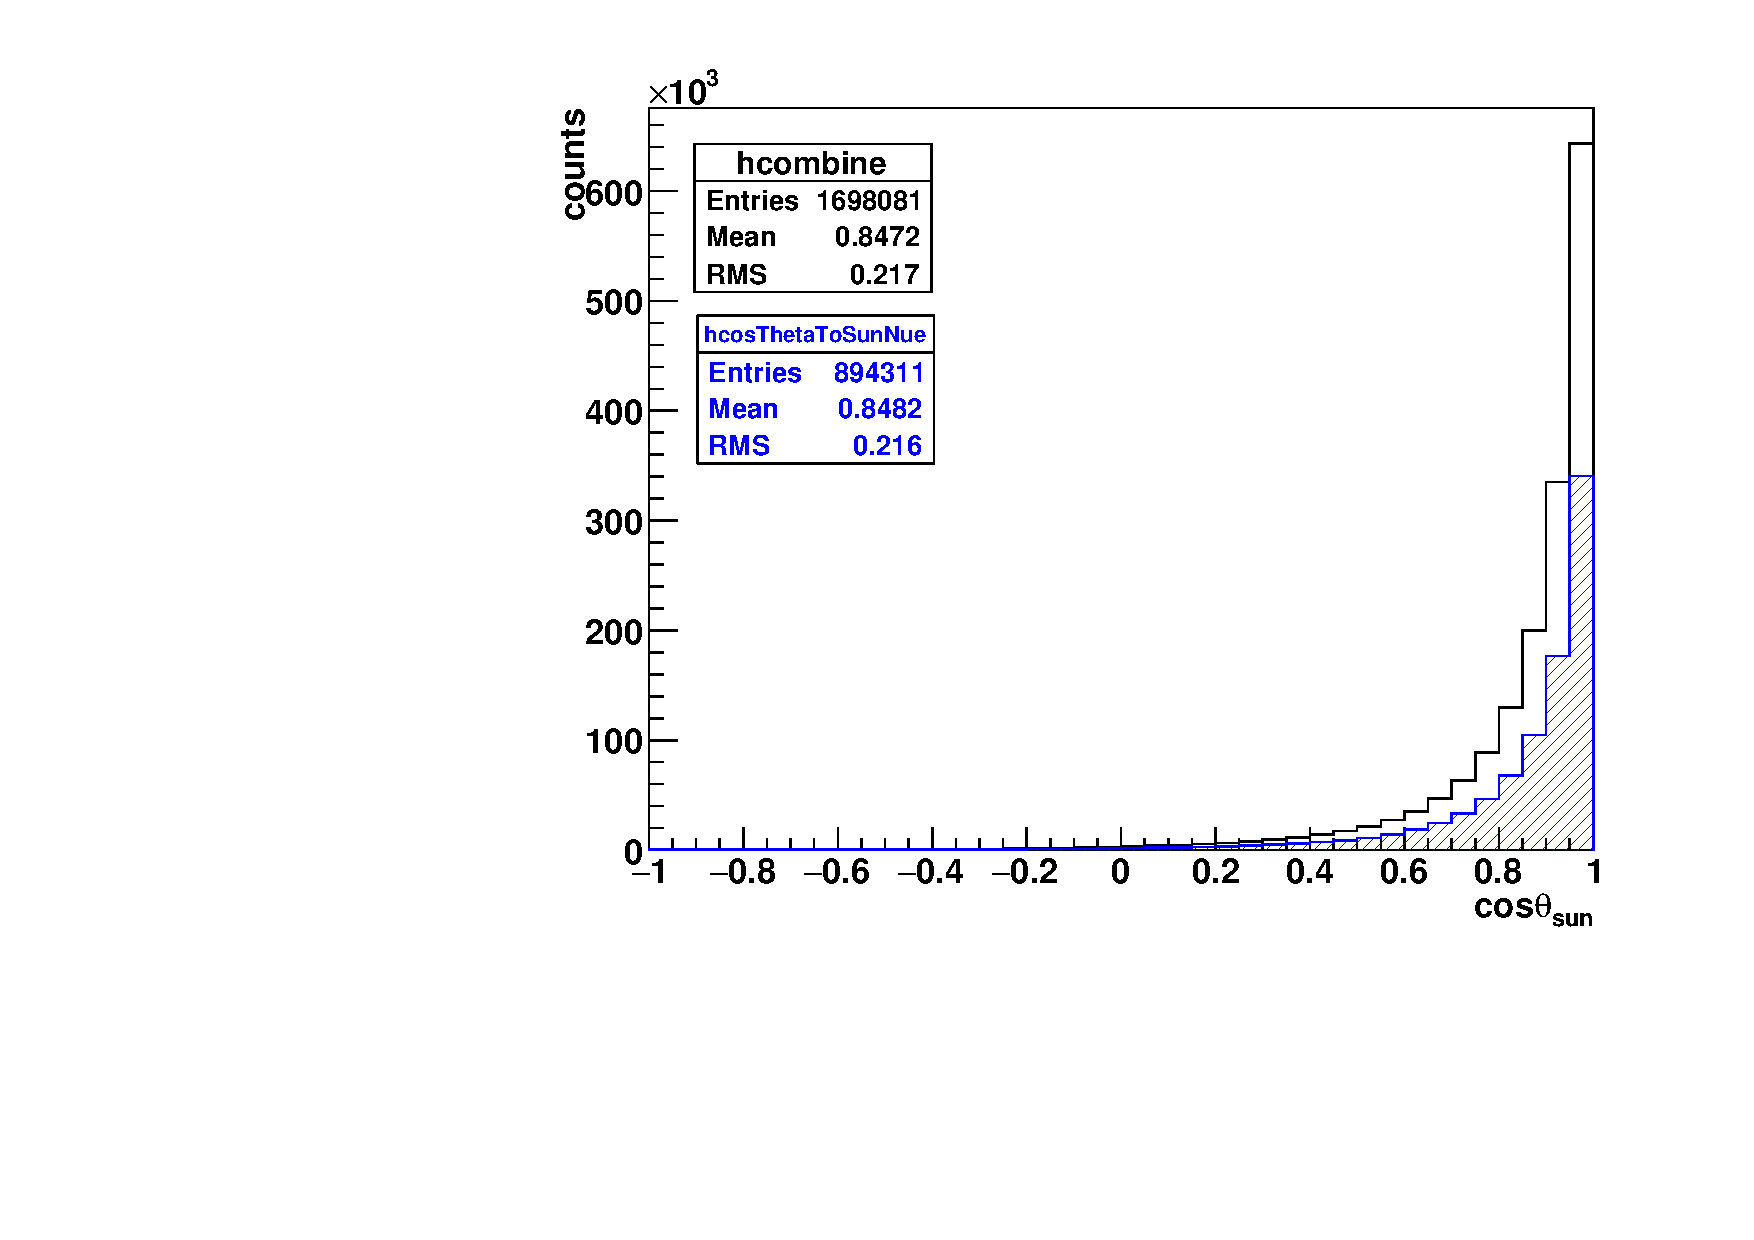
\includegraphics[width=8cm]{combine_numu_nue.pdf}
%	\caption{$\cos\theta_{sun}$ distributions from MC. The blue line is for $\nu_e$ and the black line combines solar $\nu_e$ with $\nu_\mu$.}
%	\label{combine_numu_nue}
%\end{figure} 

A software called \texttt{PSelmaa} (Physics interpretation Sun-Earth Large Mixing Angle Adiabatic
Approximation) was implemented in \texttt{RAT}\cite{fady_pselmaa}.
BS05(OP) model, normal mass hierarchy, the MSW effects from the Earth (regeneration of coherence in the Earth) are neglected. Fig.~\ref{fig:pselmaa_curves} shows the survival probability curve as a function of energies (in 0.1 MeV intervals).
\begin{figure}[!htb]
	\centering
	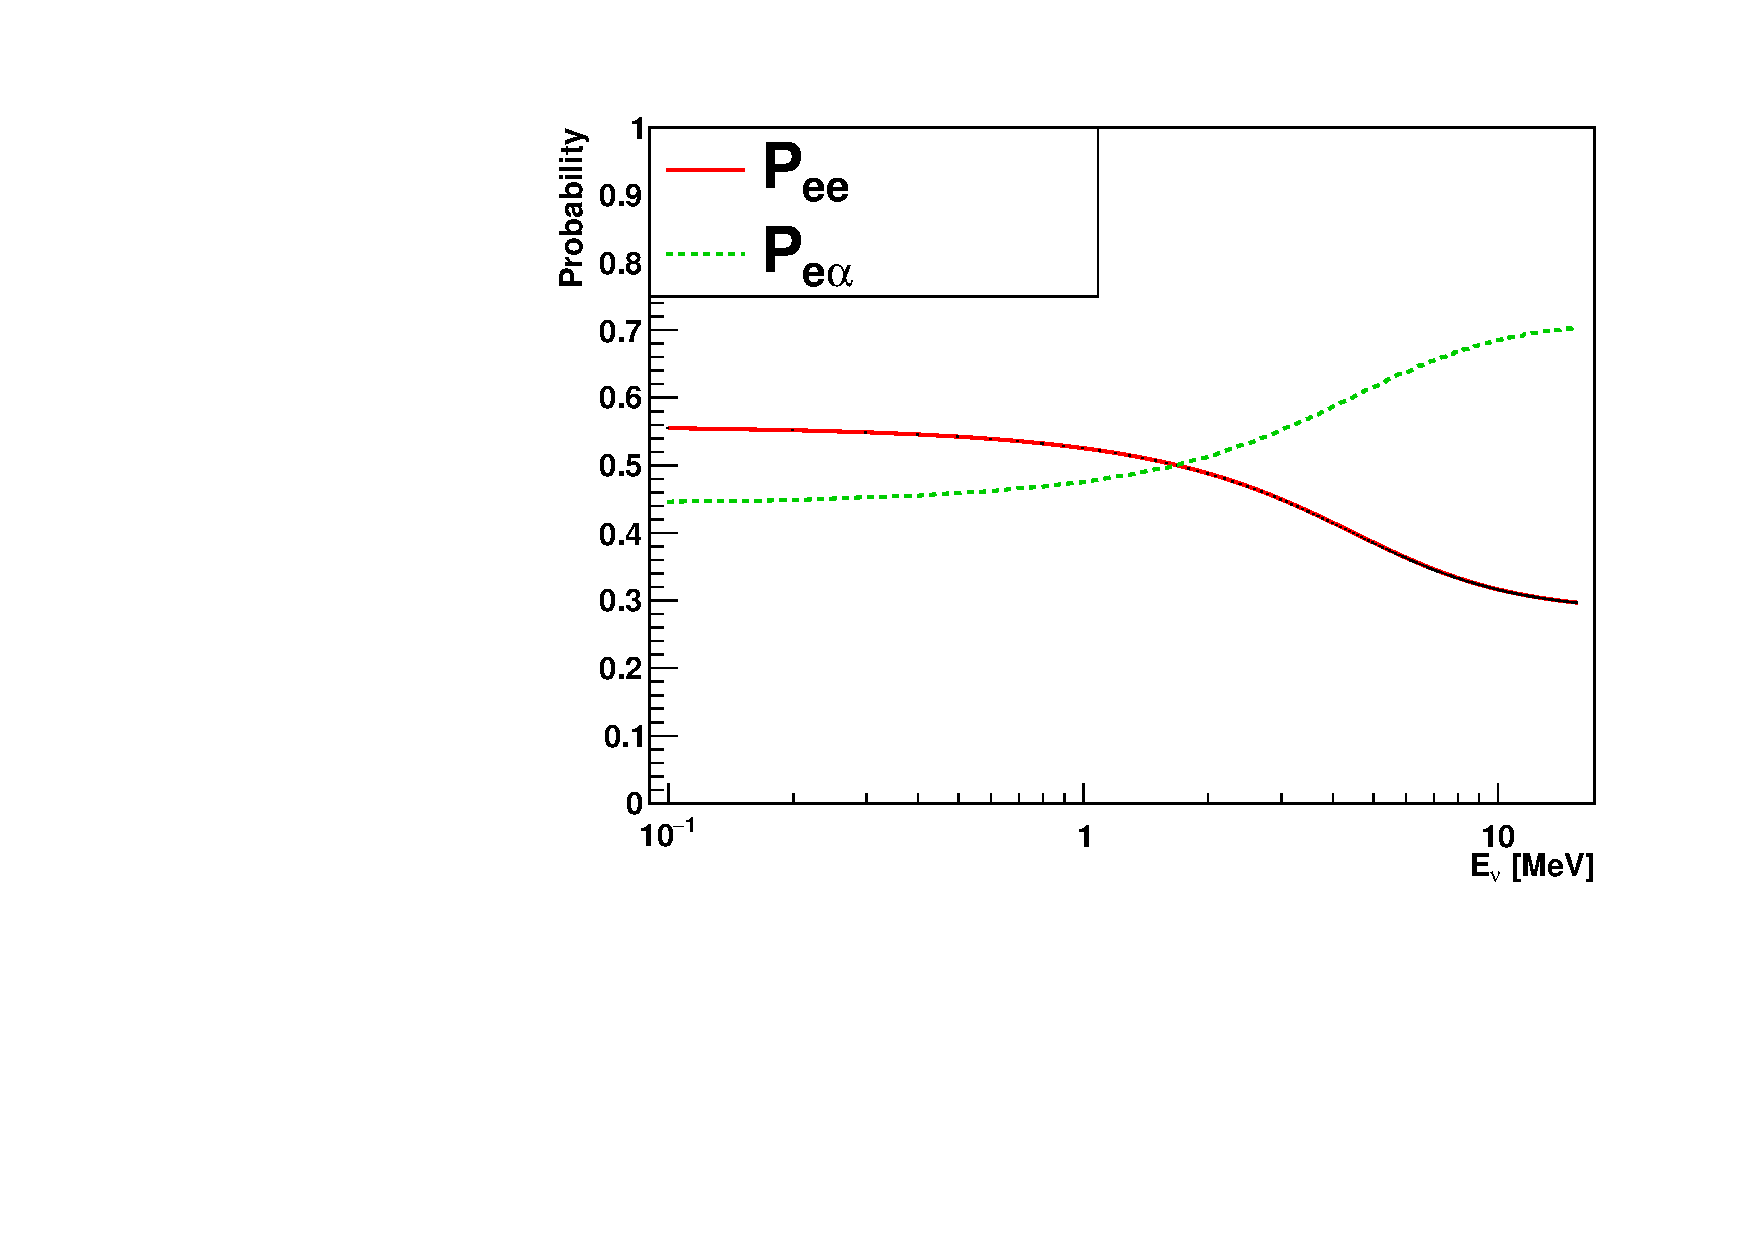
\includegraphics[width=10cm]{PSelmaa_bs05op.pdf}
	\caption{The MSW survival probability curves. The $P_{ee}$ is in solid red line and $P_{e\alpha}(=1-P_{ee}$ is in green dashed line.}
	\label{fig:pselmaa_curves}
\end{figure} 





To evaluate the $^8B$ solar neutrino flux, the fitted number of $\nu-e^-$ elastic scattering (ES) is divided by the expected number of ES and is then multiplied by the flux in the MC: 
\begin{equation}
\Phi_{^8B} = \Phi_{^8B,MC}\frac{N_{fit}}{N_{expected}},
\end{equation}

In the MC, the $\nu_e$ is generated by 1700 times the nominal; while the $\nu_\mu$ is generated by 9600 times the nominal.

Table.~\ref{table:solarNuNumbers} shows the numbers of the MC generated $\nu_e$ and $\nu_\mu$ after scaling by 1700 or 9600 as well as the BDT selections.
\begin{table}[ht]
	\centering
	\caption{Expected number of solar $\nu_e$, $\nu_\mu$ and the fitted number of signals in each energy bins.}
	\vspace{3mm}
	\label{table:solarNuNumbers}
	\begin{tabular*}{120mm}{c@{\extracolsep{\fill}}cccc}
		\toprule
		E (MeV)& $N^{expect}_{\nu_e}$ & $N^{osci.}_{\nu_e}$ & $N_{fit,sig}$\\
		\hline 
		$[5,6]$ & 68 & 26 & 26.07$\pm$5.72\\
		$[6,7]$ & 91 & 32 & 36.52$\pm$6.70\\
		$[7,8]$ & 68 & 23 & 20.87$\pm$4.95\\
		$[8,9]$ & 47 & 15 & 16.24$\pm$4.30\\
		$[9,10]$ & 30 & 10 & 11.50$\pm$3.56\\
		$[10,15]$ & 32 & 10 & 9.09$\pm$3.06\\
		$[5,15]$ & 336 & 116 & 119.40$\pm$11.84\\
		\bottomrule
	\end{tabular*}
\end{table}
%\begin{table}[ht]
%	\centering
%	\caption{Expected number of solar $\nu_e$, $\nu_\mu$ and the fitted number of signals in each energy bins.}
%	\vspace{3mm}
%	\label{table:solarNuNumbers}
%	\begin{tabular*}{155mm}{c@{\extracolsep{\fill}}cccc}
%		\toprule
%		E (MeV)& $N^{expect}_{\nu_e}$ ($N^{osci.}_{\nu_e}$) &$N^{expect}_{\nu_\mu}$ ($N^{osci.}_{\nu_\mu}$) & $N_{fit,sig}$\\
%		\hline 
%		$[5,6]$ & 68 (26) & 11 & 26.07$\pm$5.72\\
%		$[6,7]$ & 91 (32) & 14 & 36.52$\pm$6.70\\
%		$[7,8]$ & 68 (23) & 11 & 20.87$\pm$4.95\\
%		$[8,9]$ & 47 (15) & 7 & 16.24$\pm$4.30\\
%		$[9,10]$ & 30 (10) & 5 & 11.50$\pm$3.56\\
%		$[10,15]$ & 32 (10) & 5 & 9.09$\pm$3.06\\
%		$[5,15]$ & 336 (116) & 53 & 119.40$\pm$11.84\\
%		\bottomrule
%	\end{tabular*}
%\end{table}

For a nominal $^8B$ solar neutrino flux $\Phi_{MC}=5.69\times 10^6~cm^{-2}s^{-1}$, the flux is estimated to be $\Phi_{ES}=\Phi_{MC}\cdot N_{fit,sig}/(336+54./6)=1.96\pm0.20\times 10^6~cm^{-2}s^{-1}$, compared to the Super-K measurement: $\Phi_{ES}=(2.345\pm0.039)\times 10^6~cm^{-2}s^{-1}$ and the SNO+ 2018 published results: $\Phi_{ES}=2.53^{+0.31}_{-0.28}(stat.)^{+0.13}_{-0.10}(syst.)\times 10^6~cm^{-2}s^{-1}$.

Fig.~\ref{fig:fluxVsE} shows the flux as a function of energies. A $P_{ee}$ curve obtained from the \texttt{RAT} was overlay with the spectrum.
 
\begin{figure}[!htb]
	\centering
	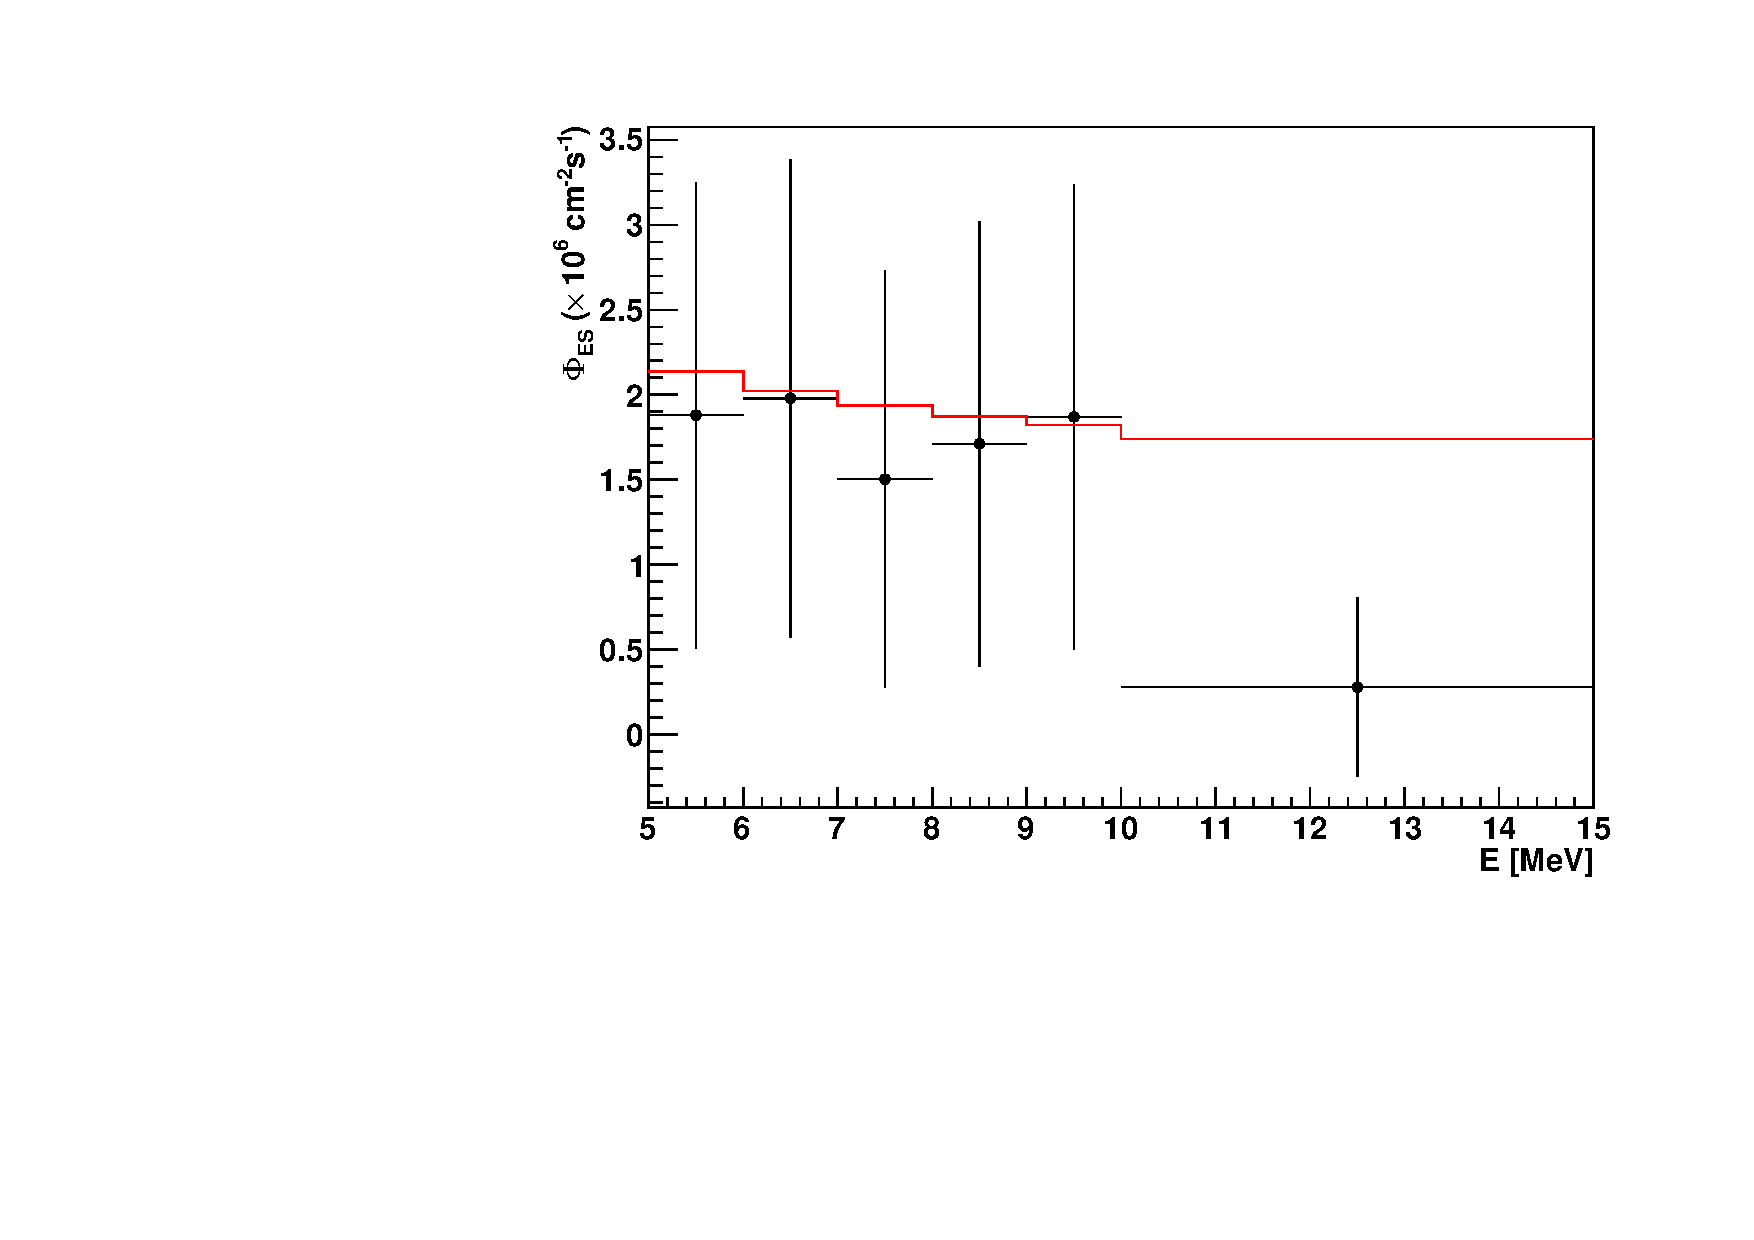
\includegraphics[width=10cm]{fluxVsEnergy.pdf}
	\caption{$^8B$ solar neutrino flux as a function of energies. The $P_{ee}$ curve obtained from the \texttt{RAT} is in red.}
	\label{fig:fluxVsE}
\end{figure}


Taking the systematics into accounts,
\begin{equation}
\Phi_{^8B,sys} = \Phi_{^8B,MC}\frac{N_{fit}}{N_{expected}}\sqrt{(\frac{N_{expected,sys}}{N_{expected}})^2+(\frac{N_{fit,sys}}{N_{fit}})^2},
\end{equation}

\subsubsection{Limits of this Study}
Here I used the background types descried in the Table.~\ref{table:mixed_MC}. However, there are a few other backgrounds, such as the backgrounds from the AV ropes, the PMTs and the cosmogenic ones mainly caused by the cosmic muons. A more comprehensive study requires to include all possible backgrounds.

For the background events, I assumed a flat distribution of $\cos\theta_{sun}$. A more realistic shape of the distribution can be investigated to describe the backgrounds more properly.  


%fractions
%efficiency